\documentclass[11pt,]{article}
\usepackage[left=1in,top=1in,right=1in,bottom=1in]{geometry}
\newcommand*{\authorfont}{\fontfamily{phv}\selectfont}
\usepackage[]{mathpazo}


  \usepackage[T1]{fontenc}
  \usepackage[utf8]{inputenc}



\usepackage{abstract}
\renewcommand{\abstractname}{}    % clear the title
\renewcommand{\absnamepos}{empty} % originally center

\renewenvironment{abstract}
 {{%
    \setlength{\leftmargin}{0mm}
    \setlength{\rightmargin}{\leftmargin}%
  }%
  \relax}
 {\endlist}

\makeatletter
\def\@maketitle{%
  \newpage
%  \null
%  \vskip 2em%
%  \begin{center}%
  \let \footnote \thanks
    {\fontsize{18}{20}\selectfont\raggedright  \setlength{\parindent}{0pt} \@title \par}%
}
%\fi
\makeatother




\setcounter{secnumdepth}{3}

\usepackage{color}
\usepackage{fancyvrb}
\newcommand{\VerbBar}{|}
\newcommand{\VERB}{\Verb[commandchars=\\\{\}]}
\DefineVerbatimEnvironment{Highlighting}{Verbatim}{commandchars=\\\{\}}
% Add ',fontsize=\small' for more characters per line
\usepackage{framed}
\definecolor{shadecolor}{RGB}{248,248,248}
\newenvironment{Shaded}{\begin{snugshade}}{\end{snugshade}}
\newcommand{\KeywordTok}[1]{\textcolor[rgb]{0.13,0.29,0.53}{\textbf{#1}}}
\newcommand{\DataTypeTok}[1]{\textcolor[rgb]{0.13,0.29,0.53}{#1}}
\newcommand{\DecValTok}[1]{\textcolor[rgb]{0.00,0.00,0.81}{#1}}
\newcommand{\BaseNTok}[1]{\textcolor[rgb]{0.00,0.00,0.81}{#1}}
\newcommand{\FloatTok}[1]{\textcolor[rgb]{0.00,0.00,0.81}{#1}}
\newcommand{\ConstantTok}[1]{\textcolor[rgb]{0.00,0.00,0.00}{#1}}
\newcommand{\CharTok}[1]{\textcolor[rgb]{0.31,0.60,0.02}{#1}}
\newcommand{\SpecialCharTok}[1]{\textcolor[rgb]{0.00,0.00,0.00}{#1}}
\newcommand{\StringTok}[1]{\textcolor[rgb]{0.31,0.60,0.02}{#1}}
\newcommand{\VerbatimStringTok}[1]{\textcolor[rgb]{0.31,0.60,0.02}{#1}}
\newcommand{\SpecialStringTok}[1]{\textcolor[rgb]{0.31,0.60,0.02}{#1}}
\newcommand{\ImportTok}[1]{#1}
\newcommand{\CommentTok}[1]{\textcolor[rgb]{0.56,0.35,0.01}{\textit{#1}}}
\newcommand{\DocumentationTok}[1]{\textcolor[rgb]{0.56,0.35,0.01}{\textbf{\textit{#1}}}}
\newcommand{\AnnotationTok}[1]{\textcolor[rgb]{0.56,0.35,0.01}{\textbf{\textit{#1}}}}
\newcommand{\CommentVarTok}[1]{\textcolor[rgb]{0.56,0.35,0.01}{\textbf{\textit{#1}}}}
\newcommand{\OtherTok}[1]{\textcolor[rgb]{0.56,0.35,0.01}{#1}}
\newcommand{\FunctionTok}[1]{\textcolor[rgb]{0.00,0.00,0.00}{#1}}
\newcommand{\VariableTok}[1]{\textcolor[rgb]{0.00,0.00,0.00}{#1}}
\newcommand{\ControlFlowTok}[1]{\textcolor[rgb]{0.13,0.29,0.53}{\textbf{#1}}}
\newcommand{\OperatorTok}[1]{\textcolor[rgb]{0.81,0.36,0.00}{\textbf{#1}}}
\newcommand{\BuiltInTok}[1]{#1}
\newcommand{\ExtensionTok}[1]{#1}
\newcommand{\PreprocessorTok}[1]{\textcolor[rgb]{0.56,0.35,0.01}{\textit{#1}}}
\newcommand{\AttributeTok}[1]{\textcolor[rgb]{0.77,0.63,0.00}{#1}}
\newcommand{\RegionMarkerTok}[1]{#1}
\newcommand{\InformationTok}[1]{\textcolor[rgb]{0.56,0.35,0.01}{\textbf{\textit{#1}}}}
\newcommand{\WarningTok}[1]{\textcolor[rgb]{0.56,0.35,0.01}{\textbf{\textit{#1}}}}
\newcommand{\AlertTok}[1]{\textcolor[rgb]{0.94,0.16,0.16}{#1}}
\newcommand{\ErrorTok}[1]{\textcolor[rgb]{0.64,0.00,0.00}{\textbf{#1}}}
\newcommand{\NormalTok}[1]{#1}
\usepackage{longtable,booktabs}

\usepackage{graphicx,grffile}
\makeatletter
\def\maxwidth{\ifdim\Gin@nat@width>\linewidth\linewidth\else\Gin@nat@width\fi}
\def\maxheight{\ifdim\Gin@nat@height>\textheight\textheight\else\Gin@nat@height\fi}
\makeatother
% Scale images if necessary, so that they will not overflow the page
% margins by default, and it is still possible to overwrite the defaults
% using explicit options in \includegraphics[width, height, ...]{}
\setkeys{Gin}{width=\maxwidth,height=\maxheight,keepaspectratio}

\title{Análisis de Geomorfométria Fluvial, Aplicado a la Cuenca Ozama,
Republica Dominicana, Utilizando Tecnología Geoespacial de Código
Abierto (Open Source)  }



\author{\Large Edel Tejeda Nova\vspace{0.05in} \newline\normalsize\emph{Agrimensor y Estudiante de Lic. en Geografia Mencion Representacion
Espacial, Universidad Autónoma de Santo Domingo (UASD)}  }


\date{}

\usepackage{titlesec}

\titleformat*{\section}{\normalsize\bfseries}
\titleformat*{\subsection}{\normalsize\itshape}
\titleformat*{\subsubsection}{\normalsize\itshape}
\titleformat*{\paragraph}{\normalsize\itshape}
\titleformat*{\subparagraph}{\normalsize\itshape}

\titlespacing{\section}
{0pt}{36pt}{0pt}
\titlespacing{\subsection}
{0pt}{36pt}{0pt}
\titlespacing{\subsubsection}
{0pt}{36pt}{0pt}





\newtheorem{hypothesis}{Hypothesis}
\usepackage{setspace}

\makeatletter
\@ifpackageloaded{hyperref}{}{%
\ifxetex
  \PassOptionsToPackage{hyphens}{url}\usepackage[setpagesize=false, % page size defined by xetex
              unicode=false, % unicode breaks when used with xetex
              xetex]{hyperref}
\else
  \PassOptionsToPackage{hyphens}{url}\usepackage[unicode=true]{hyperref}
\fi
}

\@ifpackageloaded{color}{
    \PassOptionsToPackage{usenames,dvipsnames}{color}
}{%
    \usepackage[usenames,dvipsnames]{color}
}
\makeatother
\hypersetup{breaklinks=true,
            bookmarks=true,
            pdfauthor={Edel Tejeda Nova (Agrimensor y Estudiante de Lic. en Geografia Mencion Representacion
Espacial, Universidad Autónoma de Santo Domingo (UASD))},
             pdfkeywords = {geomorfología de cuenca, cuenca Ozama, cuenca hidrográfica},  
            pdftitle={Análisis de Geomorfométria Fluvial, Aplicado a la Cuenca Ozama,
Republica Dominicana, Utilizando Tecnología Geoespacial de Código
Abierto (Open Source)},
            colorlinks=true,
            citecolor=blue,
            urlcolor=blue,
            linkcolor=magenta,
            pdfborder={0 0 0}}
\urlstyle{same}  % don't use monospace font for urls

% set default figure placement to htbp
\makeatletter
\def\fps@figure{htbp}
\makeatother

\usepackage{pdflscape} \newcommand{\blandscape}{\begin{landscape}}
\newcommand{\elandscape}{\end{landscape}}


% add tightlist ----------
\providecommand{\tightlist}{%
\setlength{\itemsep}{0pt}\setlength{\parskip}{0pt}}

\begin{document}
	
% \pagenumbering{arabic}% resets `page` counter to 1 
%
% \maketitle

{% \usefont{T1}{pnc}{m}{n}
\setlength{\parindent}{0pt}
\thispagestyle{plain}
{\fontsize{18}{20}\selectfont\raggedright 
\maketitle  % title \par  

}

{
   \vskip 13.5pt\relax \normalsize\fontsize{11}{12} 
\textbf{\authorfont Edel Tejeda Nova} \hskip 15pt \emph{\small Agrimensor y Estudiante de Lic. en Geografia Mencion Representacion
Espacial, Universidad Autónoma de Santo Domingo (UASD)}   

}

}








\begin{abstract}

    \hbox{\vrule height .2pt width 39.14pc}

    \vskip 8.5pt % \small 

\noindent La geomorfología a través de una de sus ramas llamada geomorfología
fluvial se encarga especialmente del estudio de la red y la cuenca con
múltiples fines, desatando la prevención de inundaciones y el uso
sustentable de la misma. La cuenta Ozama situada al centro-sur de la
Republica Dominicana es idónea para la realización de distintos estudios
morfométricos por tener zonas de vida, áreas protegidas y zonas de uso
urbano. Los estudios de este tipo aplicados a esta cuenca son escasos o
inexistentes, este trabajo aporta nuevos conocimientos sobre los
parámetros morfométricos de la cuenca y su red de drenaje. Todo el flujo
de trabajo se efectuó en un ambiente de software de código abierto lo
que permitirá replicar este estudio sin ningún costo.


\vskip 8.5pt \noindent \emph{Keywords}: geomorfología de cuenca, cuenca Ozama, cuenca hidrográfica \par

    \hbox{\vrule height .2pt width 39.14pc}



\end{abstract}


\vskip 6.5pt


\noindent  \section{Introducción}\label{introducciuxf3n}

La geomorfología como topografía analítica, se fundamenta en la
deducción de los antecedentes de la superficie terrestre y trata de
predecir posibles cambios en el futuro en su configuracion (Pedraza
Gilsanz, 1996). Una de las ramas de la geomorfología con mayor
desarrollo en las últimas décadas, es la geomorfología fluvial, que se
encarga del estudio de los sistemas fluviales, especialmente la red y la
cuenca.

Una cuenca hidrográfica es una unidad morfológica que está delimitada de
forma natural en donde sus aguas superficiales convergen hacia un lecho
fluvial, y por medio de una red de cauces principales fluyen al
mar(Gaspari, Rodríguez Vagaría, Senisterra, Delgado, \& Besteiro, 2013).

Los estudios morfométricos de cuencas y redes de drenaje, aportan
conocimiento sobre el comportamiento morfodinámico e hidrológico,
contribuyendo así al diseño informado de medidas de prevención en
escenarios de abundantes precipitaciones, así como a la planificación
del uso sustentable de la misma (Domínguez et al., 2003). Por otra parte
Arriaga-Cabrera et al. (2009) resalta que el estudio de una cuenca es un
avance para las políticas de administración sustentable porque en la
actualidad no existen estudios que explique el comportamiento hídrico y
morfométrico que permitan determinar y predecir su dinámica.

La cuenca del río Ozama, situada al sur-centro del República Dominicana,
es idónea para distintos estudios, dado que es una cuenca modelo por
múltiples razones: 1) Es una de las principales en términos ecológicos,
porque existen en ella tres zonas de vida y dos zonas de transición en
donde interactúan diferentes tipos de flora y fauna; 2) Se han declarado
varias áreas protegidas dentro de la cuenca; 3) Una parte importante de
su superficie incluye terrenos destinados para uso urbano, pero con
preencia también destacada de la agricultura y la ganadería
(Medio-Ambiente, 2012). Si bien se trata de una cuenca importante para
el país y para el entorno urbano, su escasa instrumentación impone retos
añadidos al conocimiento de sus procesos específicos. Sin embargo, con
las técnicas y la información de elevación disponibles actualmente, es
posible profundizar en el conocimiento de esta cuenca mediante estudios
morfométricos aplicados a geomorfología fluvial utilizando herramientas
de bajo costo.

En la Republica dominicana los estudios de geomorfología fluvial son
escasos y dispersos. La cuenca del río Ozama no escapa a esta realidad,
y sólo cuenta con estudios generales y, aunque existe información
geológica, no existen análisis morfométricos de la misma. Este trabajo
aporta nuevo conocimiento sobre la red de drenaje del Ozama (e.g.~orden
de red, análisis hortoniano, análisis de cursos más largos para
determinar perfiles longitudinales e índices de concavidad), e
igualmente estudia la delimitación de la cuenca y subcuencas a partir de
algoritmos de dirección. En todo el flujo de trabajo, se empleó software
de código abierto (\emph{open source}), y se generaron productos
mediante \emph{script} reproducible, lo que permitirá replicar este
estudio sin ningún costo.

Es una cuenca importante pero poco instrumentada, la exploración visual
de la misma revela patrones que despiertan la curiosidad. Concretamente,
la cuenca del río Ozama tiene una forma peculiar (e.g.~de perímetro muy
rectilíneo), y su red de drenaje presenta unas características bastante
llamativas (e.g.~cursos de largo desarrollo, perfiles de elevación muy
variables).

En este sentido, interesa conocer cuáles son los controles que explican
su morfología, por qué determinados sectores de la misma presentan
evidencia preliminar de procesos de reorganización del drenaje y, en su
caso, formular una o varias hipótesis que expliquen estos fenómenos.
Comúnmente, la morfometría de cuenca deja señales inequívocas
(e.g.~hipsometría) con las cuales interpretar posibles controles
litológicos y estructurales. La caracterización de la red de drenaje
definida por el método de Horton resalta la existencia (si los hubiere)
de patrones en el orden de red y en la forma de las redes de drenaje
según sus órdenes. Si la cuenca Ozama llegara a presentar algún patrón,
conoceremos de qué factores o elementos dependen.

Según Horton (1945) comúnmente la razón de bifurcación es constante para
todos los órdenes de red de una cuenca. Uno de los objetivos es
determinar si este fenómeno ocurre en nuestra cuenca de estudio y si
difiere la razón de bifurcación calculada por medio de coeficientes de
regresión, de la creada por el promedio de las razones de bifurcación de
cada par de órdenes de red, tratando de explicar las grandes diferencias
que puedan surgir.

La configuración espacial resultado de los análisis aplicados a los
perfiles longitudinales y los índices de concavidad de los cursos más
largos de una cuenca, muy a menudo arrojan que se relacionan con la
litología, por lo que, el análisis aplicado a la cuenca Ozama persigue
comprobar si su curso más largo se rige bajo este criterio y si existe
alguna evidencia en la cuenca Ozama de uno o varios fenómenos de
reorganización del drenaje.

\section{Metodología}\label{metodologuxeda}

Para responder las preguntas de investigación, en este estudio se
recopilaron datos de elevación, conocimiento de terreno y productos
cartográficos, todos referidos a la cuenca del río Ozama y su entorno.
Dichas fuentes fueron procesadas con algoritmos de morfometría fluvial
dentro de un ambiente de programación estadística, para obtener las
principales tendencias.

\subsection{Área de Estudio}\label{uxe1rea-de-estudio}

La cuenca del río Ozama abarca una superficie de 2,847.15 kilometros
cuadrados, se encuentra ubicada entre las coordendas geográficas de
18º58'30.393" N y 18º23'40.846" N latitud norte y 70º16'5.369" W y
69º24'27.891" W longitud oeste (Medio-Ambiente, 2012). Por su tamaño, es
la cuarta cuenca mas grande de la República Dominicana, y en cuanto a
longitud de curso más largo es la TERCERA (Gutiérrez, 2014). Según
Medio-Ambiente (2012), el río nace en la Loma Palo Bonito (loma Siete
Cabezas), la cual forma parte de la sierra de Yamasa. (Ver figura
\ref{fig:ubi-indrhi})

\begin{figure}
\centering
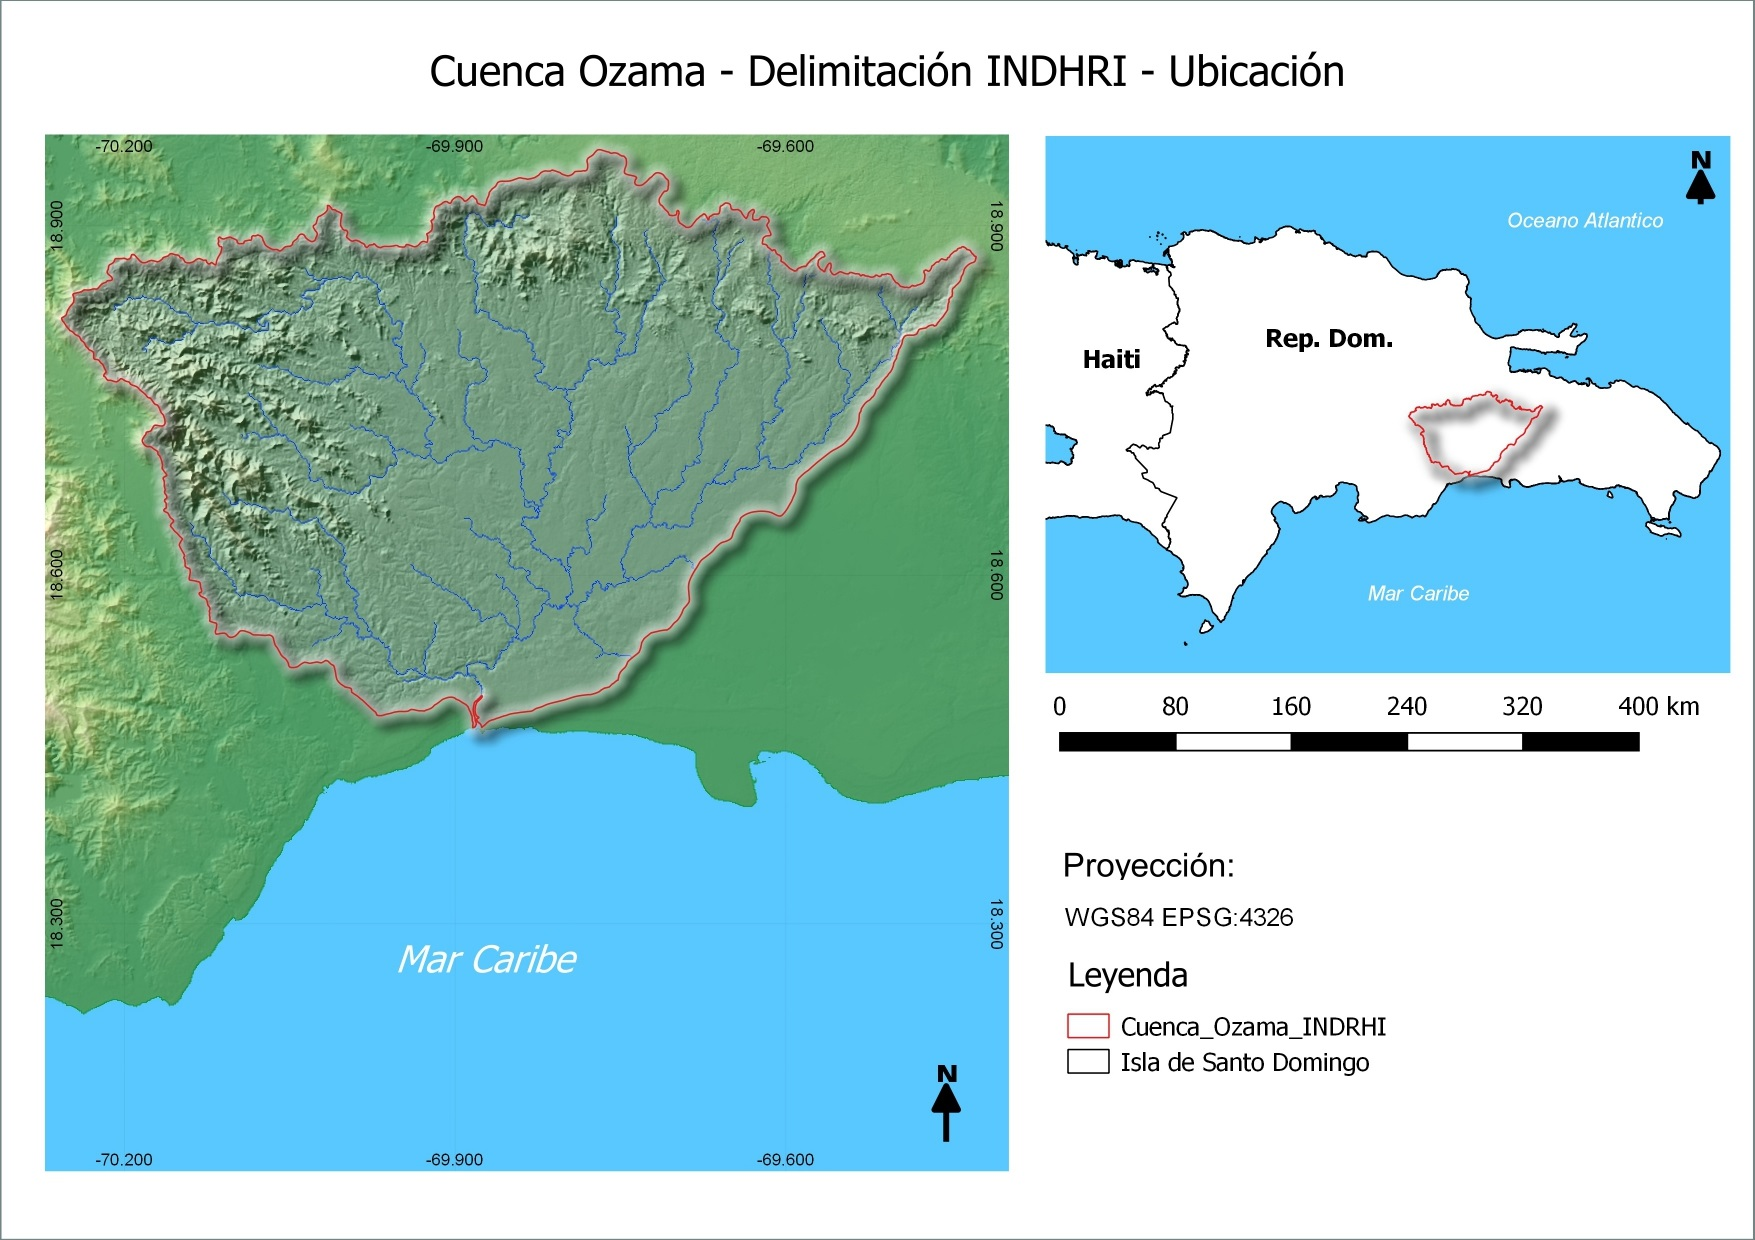
\includegraphics[width=0.75000\textwidth]{Productos Generados/Mapa Final_page-0001.jpg}
\caption{\label{fig:ubi-indrhi}Ubicacion cuenca Ozama}
\end{figure}

Cubre el área geomórfica de la Llanura Costera del Caribe, incluyendo
áreas de roca de tipo caliza de arrecifes costeros y depósitos aluviales
y de origen lacustre marino, con una superficie de
1,719.65,km\textsuperscript{2} (61.60\%). La zona montañosa comprende la
cordillera oriental, la región de la Sierra de Yamasá y la llanura
montañosa de Los Haitises, con una superficie de
1,072.40,km\textsuperscript{2} (38.40 \%). El tipo geológico está
compuesto por materiales sedimentarios, diversos arrecifes, grava,
conglomerado (tipo Santo Domingo en La Romana), calizas grises tipo
Hatillo, sedimentos aluviales de lagos oceánicos en cauces fluviales,
terrazas planicies aluviales y valles (Medio-Ambiente, 2012).

\subsection{Fuentes de datos y
métodos}\label{fuentes-de-datos-y-muxe9todos}

Para el estudio y análisis de la cuenca Ozama, se calcularon sus
parámetros morfométricos, abarcando aspectos de los atributos de la red
y de la cuenca. Todos los cálculos se efectuaron utilizando el flujo de
trabajo de semiprocesamiento automático usando GRASS GIS en R (José
Ramón Martínez Batlle, 2020), a través del paquete rgrass7 (Bivand,
2019; Martínez Batlle, 2020).

Se utilizó un modelo digital de elevación (DEM) espacial existente
(SRTM3 v2.1 y AW3D-30m v1), mejorado con el algoritmo \emph{Multi-Error
Removed Improved Terrain (MERIT)}, el cual eliminó y corrigió los
errores de orientación absoluta, ruido de rayas, ruido de moteado y
orientación de altura de árbol (Yamazaki, 2018). Este MERIT DEM fue
descargado del sitio web de Dai YAMAZAKI's
(\url{http://hydro.iis.u-tokyo.ac.jp/~yamadai} ). También se utilizaron
multiples complementos de GRASS GIS para calcular los parámetros
morfométricos, entre los que destacan \texttt{r.watershed},
\texttt{r.stream*} and \texttt{r.basin} (Martínez Batlle, 2020).

El flujo de trabajo consistió en crear región y localización de GRASS
tomando como referencia la extensión y el sistema de coordenadas del
DEM. Posteriormente, se generaron el límite de la cuenca utilizando el
complemento de GRASS \texttt{r.water.outlet}.

Para obtener los cursos más largos de la cuenca Ozama y los cursos más
largo de sus cuencas tributarias así como sus perfiles de
longitudinales, sus índices de concavidad y sus curvas hipsométricas se
ejecutaron una serie de scrits, que forman parte de la guía creada por
Martínez Batlle (2020).

\section{Resultados}\label{resultados}

Una vez finalizada la ejecución de los algoritmos de medición de
morfología fluvial, se obtuvieron una serie de informaciónes que
ayudarán a dar respuesta a las preguntas de investigaciones y a
comprender los detalles de los parámetros geomorfológicos de la Cuenca
de Ozama.

\subsection{Delimitación y Forma}\label{delimitaciuxf3n-y-forma}

La cuenca extraída en este estudio alcanzó ca.
3,400,km\textsuperscript{2} y un perímetro de 420,km. Estas cifras
contrastan con las calculadas a partir del polígono de delimitación del
INDRHI, cuyos valores de área y perímetro fueron de
2,740,km\textsuperscript{2} y 300,km, respectivamente. En cuanto a
forma, la cuenca extraída en este estudio se extiende hacia el este
sobrepasando, por mucho, los límites de la cuenca del INDRHI (Ver figura
\ref{fig:delimitacioncuencaindrhi} y 2).

\begin{figure}
\centering
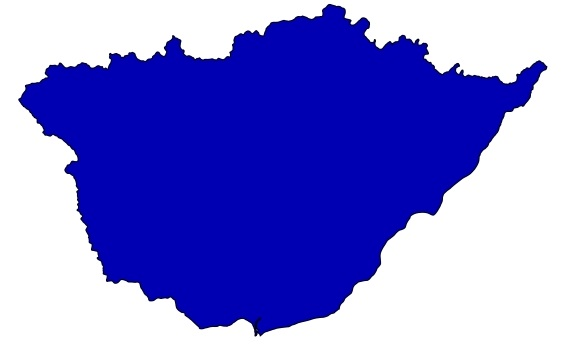
\includegraphics[width=0.75000\textwidth]{Productos Generados/Cuenca_forma1.jpeg}
\caption{\label{fig:delimitacioncuencaindrhi}Delimitacion Cuenca Rio
Ozama (INDRHI)}
\end{figure}

\begin{figure}
\centering
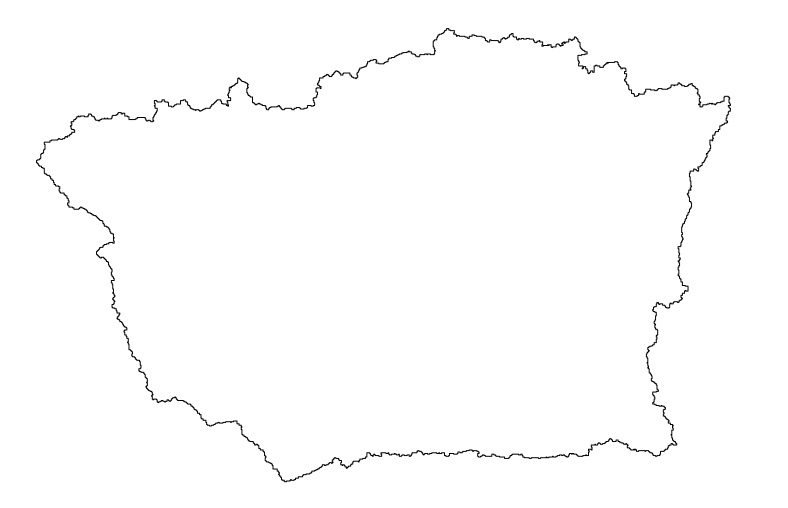
\includegraphics[width=0.75000\textwidth]{Productos Generados/Cuenca_p_forma1.jpeg}
\caption{\label{fig:delimitacioncuencaindrhi}Delimitacion Cuenca Rio
Ozama}
\end{figure}

\subsection{Datos de Elevación y
Pendiente}\label{datos-de-elevaciuxf3n-y-pendiente}

La cuenca del río Ozama alcanza como elevación maxima aprox. 900 metros
sobre el nivel del mar, con promedio de 110 metros, mediana en 60 metros
y un valor minimo de 0 metros con fuerte sesgo a la derecha (Ver figura
\ref{fig:hist1}). Esto implica que la mayor parte de las elevaciones de
la cuenca del rio ozama son bajas.

\begin{figure}
\centering
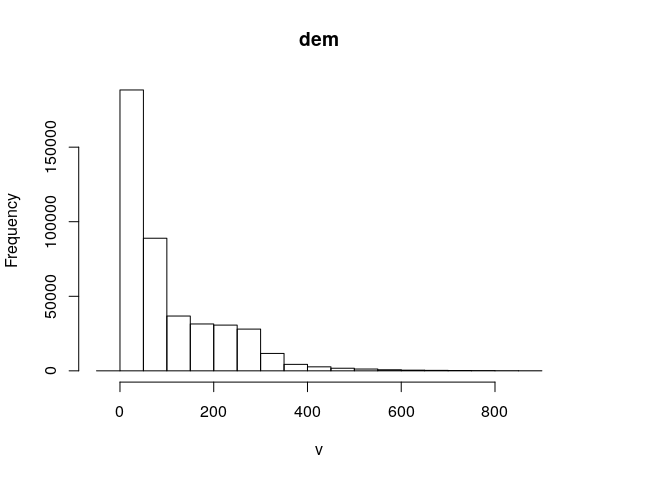
\includegraphics[width=0.75000\textwidth]{Productos Generados/Histograma-de-elevaciones.png}
\caption{\label{fig:hist1}Histograma de elevaciones}
\end{figure}

La pendiente máxima de la cuenca del río Ozama es de aproximadamente 45
grados, la pendiente promedio es de 37 grados, la mediana es de 20
grados y la mínima es de 0 grados (Ver figura \ref{fig:hist2}). La
cuenca ozama cuenta con pendientes que desde el punto de vista
agropecuario se corresponden a los mejores suelos para su
aprovechamiento mientras que los procesos erosivos y los movimientos de
masas son menores.

\begin{figure}
\centering
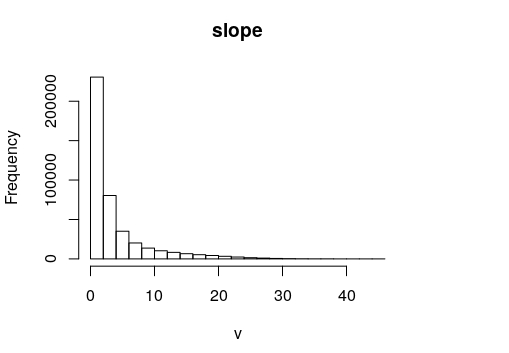
\includegraphics[width=0.75000\textwidth]{Productos Generados/slope.jpeg}
\caption{\label{fig:hist2}Histograma de pendiente}
\end{figure}

\subsection{Red de Dranaje, Orden de red y análisis
hortoniano}\label{red-de-dranaje-orden-de-red-y-anuxe1lisis-hortoniano}

Partiendo de su cauce principal se generó la red de drenaje de la cuenca
del rio Ozama (Ver figura \ref{fig:drenaje}), la cual tiene un orden de
red mínimo de 1 y un máximo de 7, según el método de Horton aplicado
para determinar su grado de ramificación (Horton, 1945) (Ver figura
\ref{fig:C_O}).

\begin{figure}
\centering
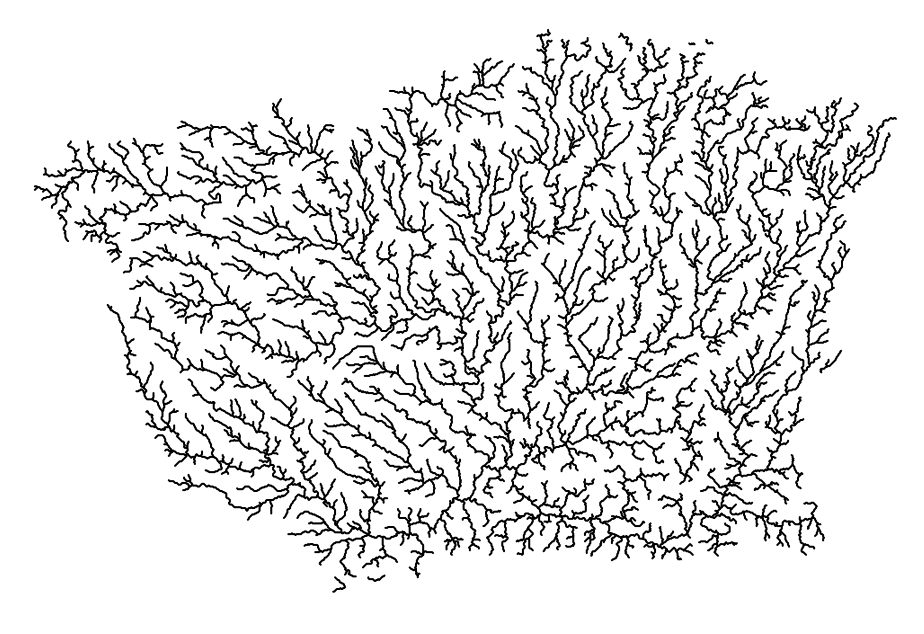
\includegraphics[width=0.75000\textwidth]{Productos Generados/Red_drenaje_ozama.png}
\caption{\label{fig:drenaje}Red de drenaje de la cuenca Ozama}
\end{figure}

\begin{figure}
\centering
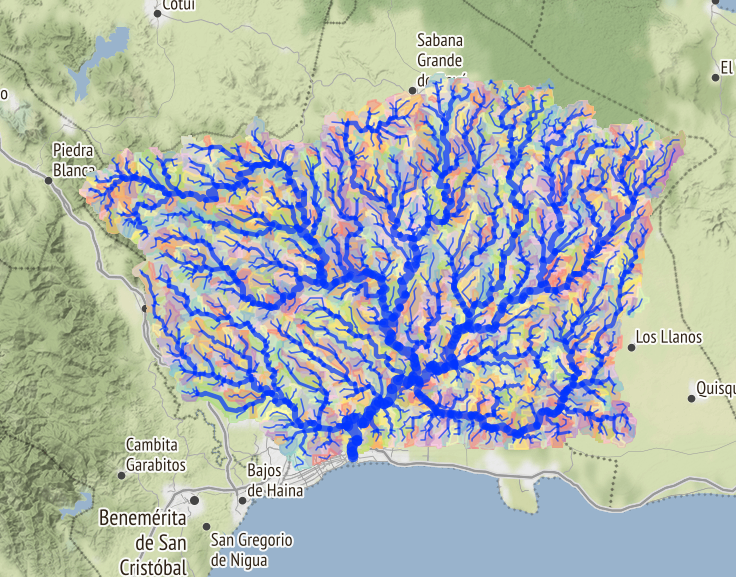
\includegraphics[width=0.75000\textwidth]{Productos Generados/cuencas_y_orden_de_red_salida1.png}
\caption{\label{fig:C_O}Cuenca Ozama y su red de drenaje}
\end{figure}

\subsubsection{Razón de bifurcación promedio para cada par de ordenes de
red}\label{razuxf3n-de-bifurcaciuxf3n-promedio-para-cada-par-de-ordenes-de-red}

Aplicando el addon de GRASS GIS \texttt{r.stream.stats} se obtuvieron
las estadísticas por orden de red, esta muestra que la cuenca del rio
Ozama tiene 1,328 cursos fluviales de orden 1, 274 de orden 2, 63 de
orden 3, 13 de orden 4, 5 de orden 5, 2 de orden 6 y 1 de orden 7. La
razón de bifurcación para el par de ordenes 1-2 es 1,328/274=4.846, para
el par 2-3 es 274/63=4.349, para el par 3-4 es 63/13=4.846, para el par
4-5 es 13/5=2.600, para el par 5-6 es 5/2=2.500, para el par 6-7 es
2/1=1. El valor promedio sería Rb=3.523679 (Ver Tabla \ref{tab:tabla}).

\newpage   

\begin{longtable}[]{@{}cc@{}}
\caption{Ordenes de red con sus repectivos cursos
fluviales\label{tab:tabla}}\tabularnewline
\toprule
Orden & No. de Cursos\tabularnewline
\midrule
\endfirsthead
\toprule
Orden & No. de Cursos\tabularnewline
\midrule
\endhead
1 & 1,328\tabularnewline
2 & 274\tabularnewline
3 & 63\tabularnewline
4 & 13\tabularnewline
5 & 5\tabularnewline
6 & 2\tabularnewline
7 & 1\tabularnewline
\bottomrule
\end{longtable}

\subsubsection{Razón de bifurcación calculada por medio de coeficientes
de
regresión}\label{razuxf3n-de-bifurcaciuxf3n-calculada-por-medio-de-coeficientes-de-regresiuxf3n}

Ya obtenido el numero de cursos fluviales y el modelo generado con
dichos datos se creo la pendiente de la recta para calcular la razon de
bifurcación, obteniendo como resultado Rb=3.361632 (Ver figura
\ref{fig:Rb_R}).

\begin{figure}
\centering
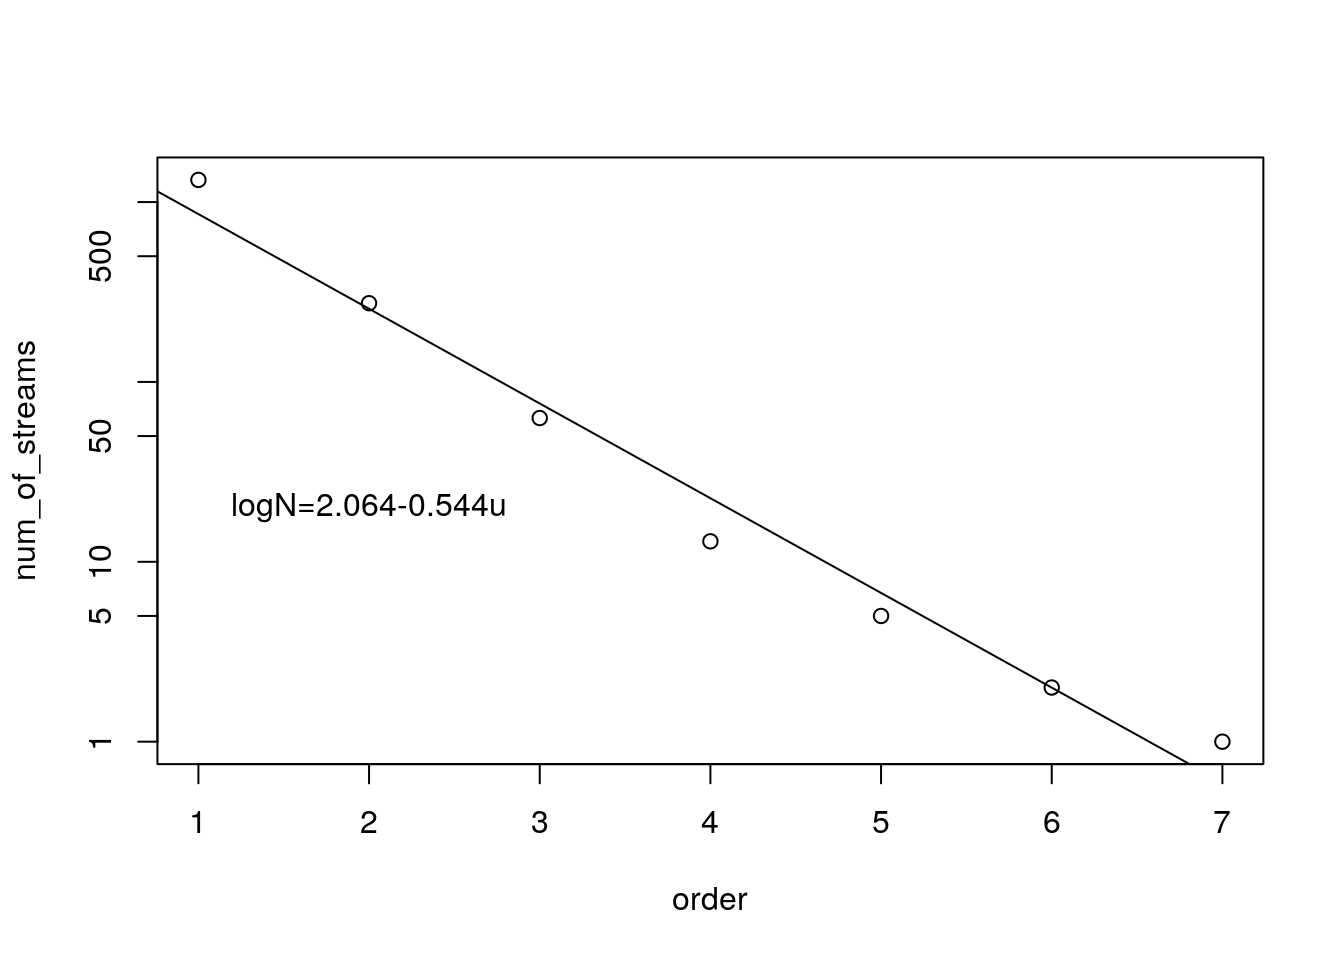
\includegraphics[width=0.75000\textwidth]{Productos Generados/Orden_red_regresion.png}
\caption{\label{fig:Rb_R} Recta de regresión para el modelo ``numero de
curso fluviales en función del orden de red'' y ecuación
correspondiente}
\end{figure}

\subsection{Perfiles Longitudinales e Índices de
Concavidad}\label{perfiles-longitudinales-e-uxedndices-de-concavidad}

La complejidad de la Cuenca Ozama obligo a que este análisis se
dividiera en seis partes, estas se corresponden a subcuentas que se
definieron para abarcar todos los perfiles longitudinales con sus
valores de concavidad.

\subsubsection{Subcuenta Principal Rio
Ozama}\label{subcuenta-principal-rio-ozama}

Los perfiles longitudinales de los cursos fluviales que drenan la
subcuenca principal Rio Ozama, presentan características similares,
tales como en el rango de valores de concavidad. Un detallado análisis
permite observar 5 grupos de tendencias, en donde el grupo uno (1)
presenta errores en desembocadura y cabecera que pudieran ser
ocasionados por DEM, el grupo dos (2) muestra meseta en cabecera,
provocando índices de concavidad negativos (convexos), el tercer grupo
(3) es formado por los que tienen concavidad perfecta, el cuarto (4)
grupo se caracteriza por cambios que pudieran ocurrir en la litología,
formando los llamados sifones, por último se observan perfiles con
índices de concavidad cercanos a cero, estos forman el grupo número
cinco (5) y abarcan los perfiles rectilíneos (Ver figura
\ref{fig:LFP_Ozama0}, \ref{fig:LFP_Ozama1} y \ref{fig:LFP_Ozama2}). Los
perfiles longitudinales cóncavos son muy pronunciados y los más
frecuentes en la subcuenca principal Rio Ozama.

\begin{figure}
\centering
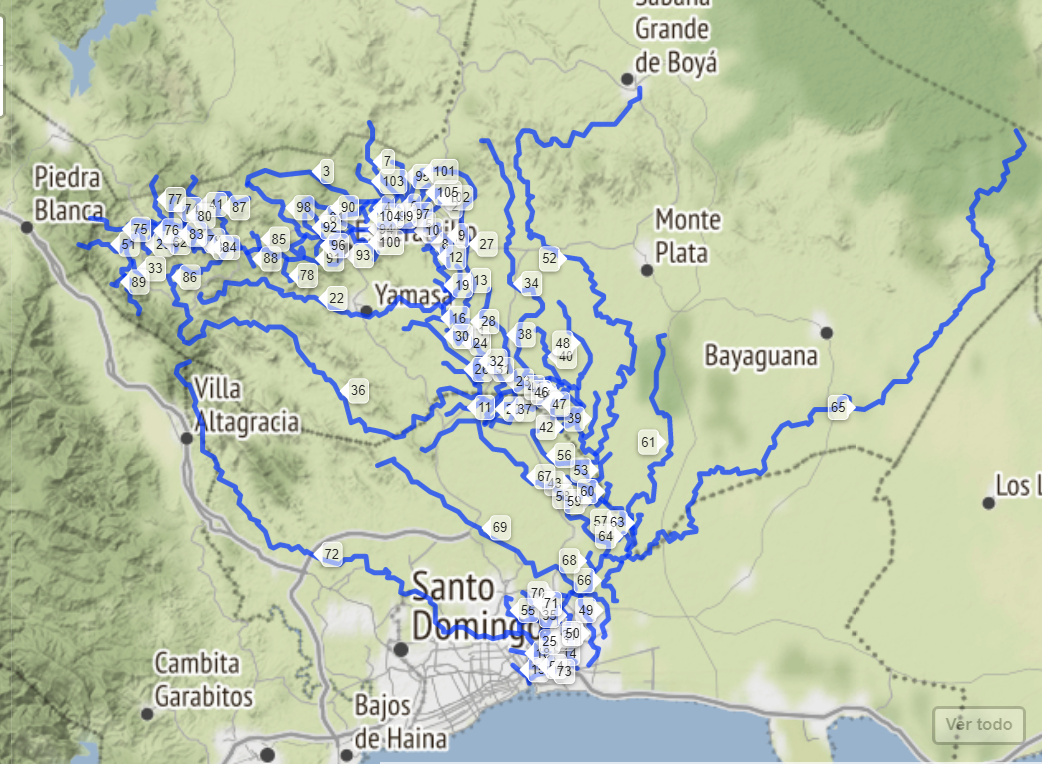
\includegraphics[width=0.65000\textwidth]{Productos Generados/Perfil1.png}
\caption{\label{fig:LFP_Ozama0} Subcuenta principal Rio Ozama}
\end{figure}

\begin{figure}
\centering
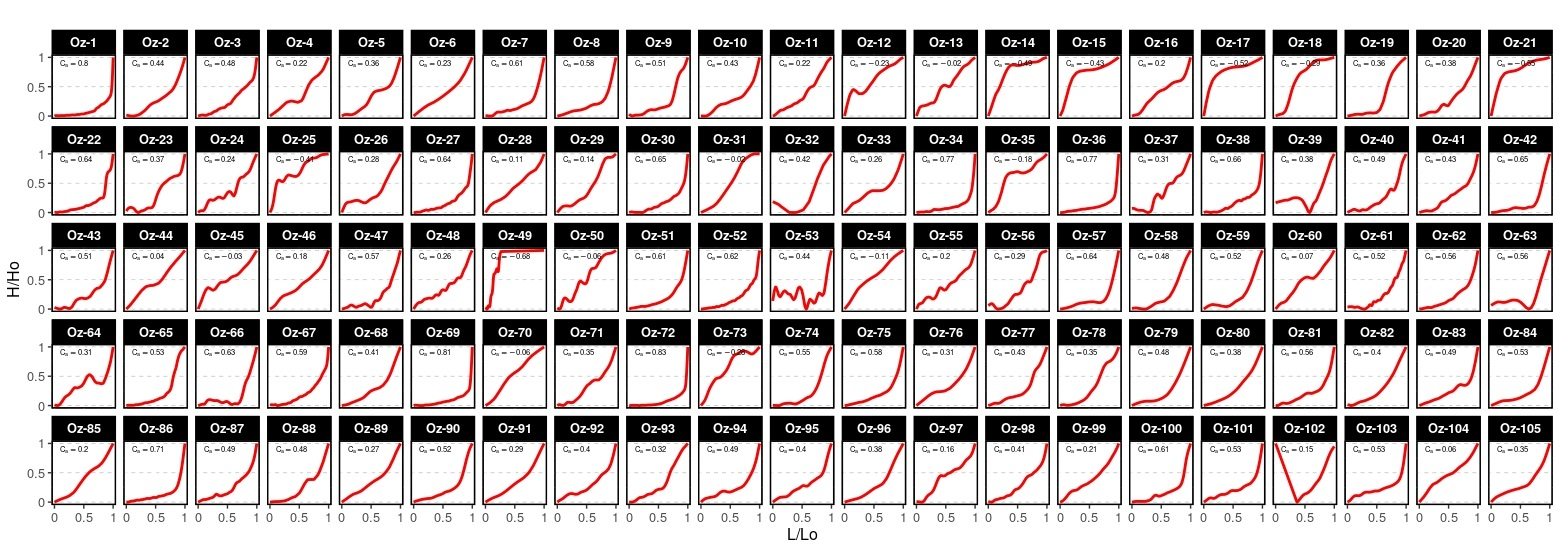
\includegraphics[width=1.00000\textwidth]{Productos Generados/perfiles_adimensionales_indices_de_concavidad.jpeg}
\caption{\label{fig:LFP_Ozama1} Perfiles Longitudinales e Indices de
Concavidad de la subcuenta principal Rio Ozama}
\end{figure}

\begin{figure}
\centering
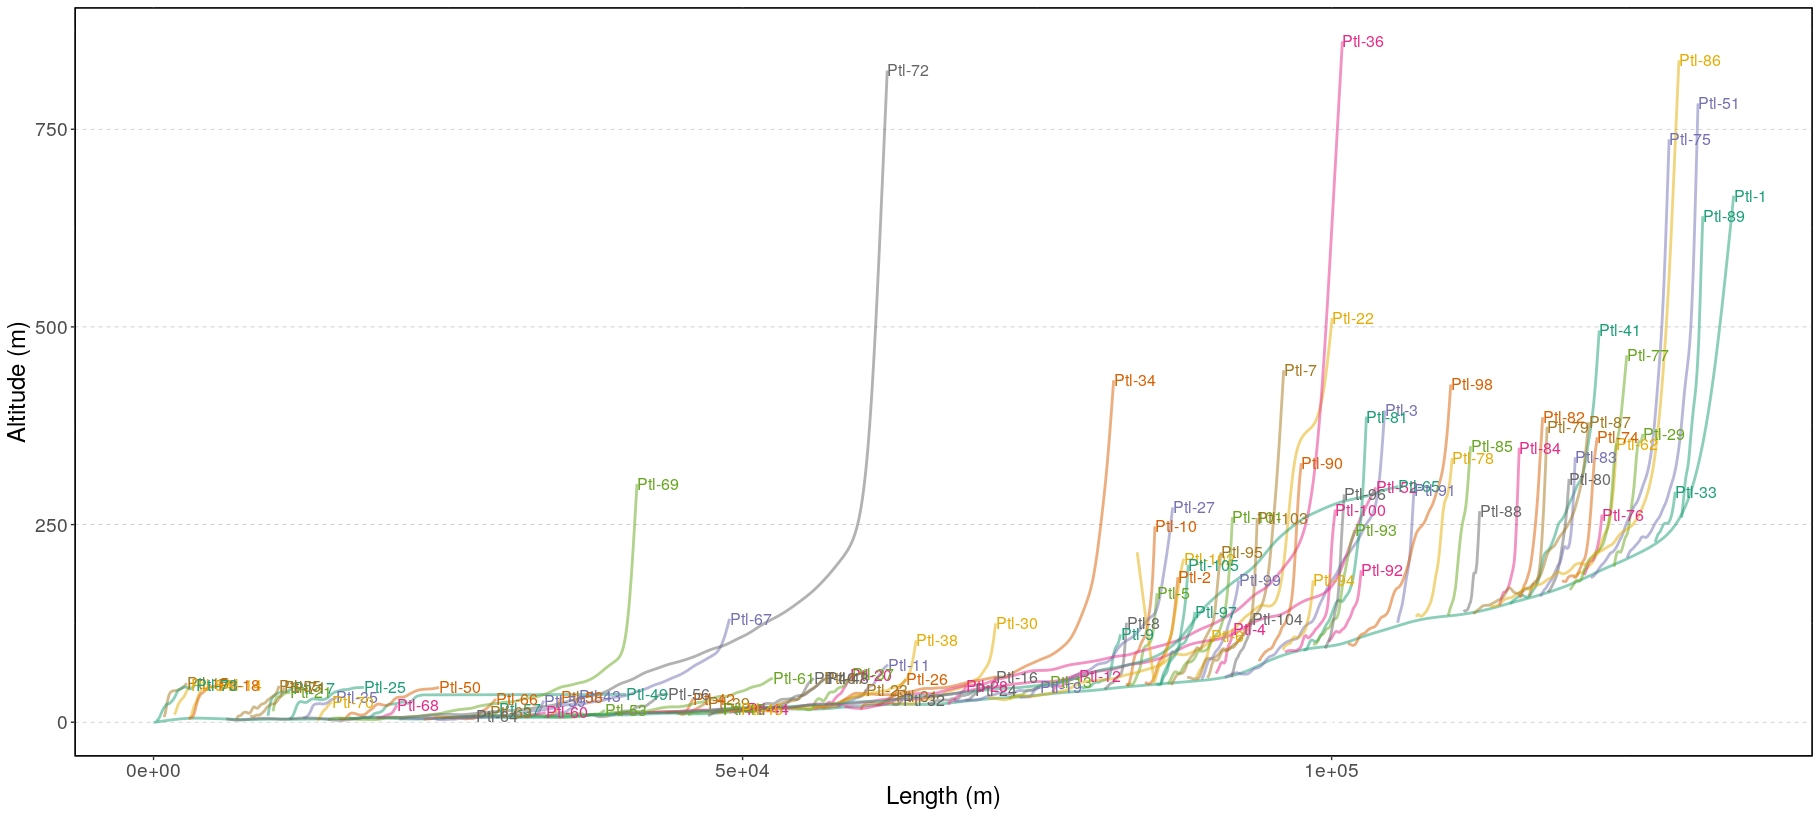
\includegraphics[width=1.00000\textwidth]{Productos Generados/perfiles_todos_juntos.jpeg}
\caption{\label{fig:LFP_Ozama2} Todos los Perfiles de elevación de la
subcuenta principal Rio Ozama}
\end{figure}

\newpage

\subsubsection{Subcuenca Rio Yabacao}\label{subcuenca-rio-yabacao}

En la subcuenca Rio Yacao al igual que en la subcuenca principal del Rio
Ozama, los patrones de perfiles rectilíneos, concavidad perfecta,
perfiles convexos y los perfiles de sifones están presentes, predominado
de entre ellos los perfiles cóncavos.(Ver figura \ref{fig:LFP_yabacao0},
\ref{fig:LFP_yabacao1} y \ref{fig:LFP_yabacao2}).

\begin{figure}
\centering
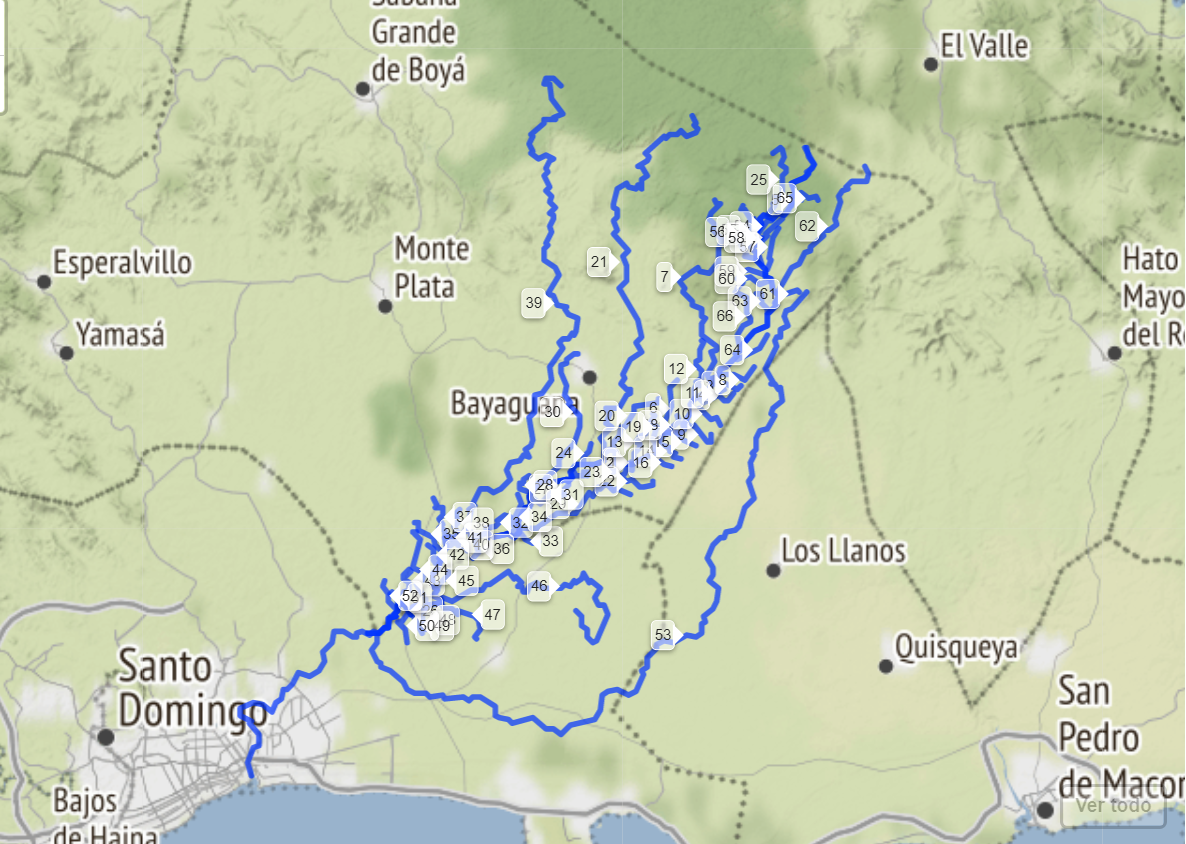
\includegraphics[width=0.65000\textwidth]{Productos Generados/p_yabacao.png}
\caption{\label{fig:LFP_yabacao0} Subcuenta Rio Yabacao}
\end{figure}

\begin{figure}
\centering
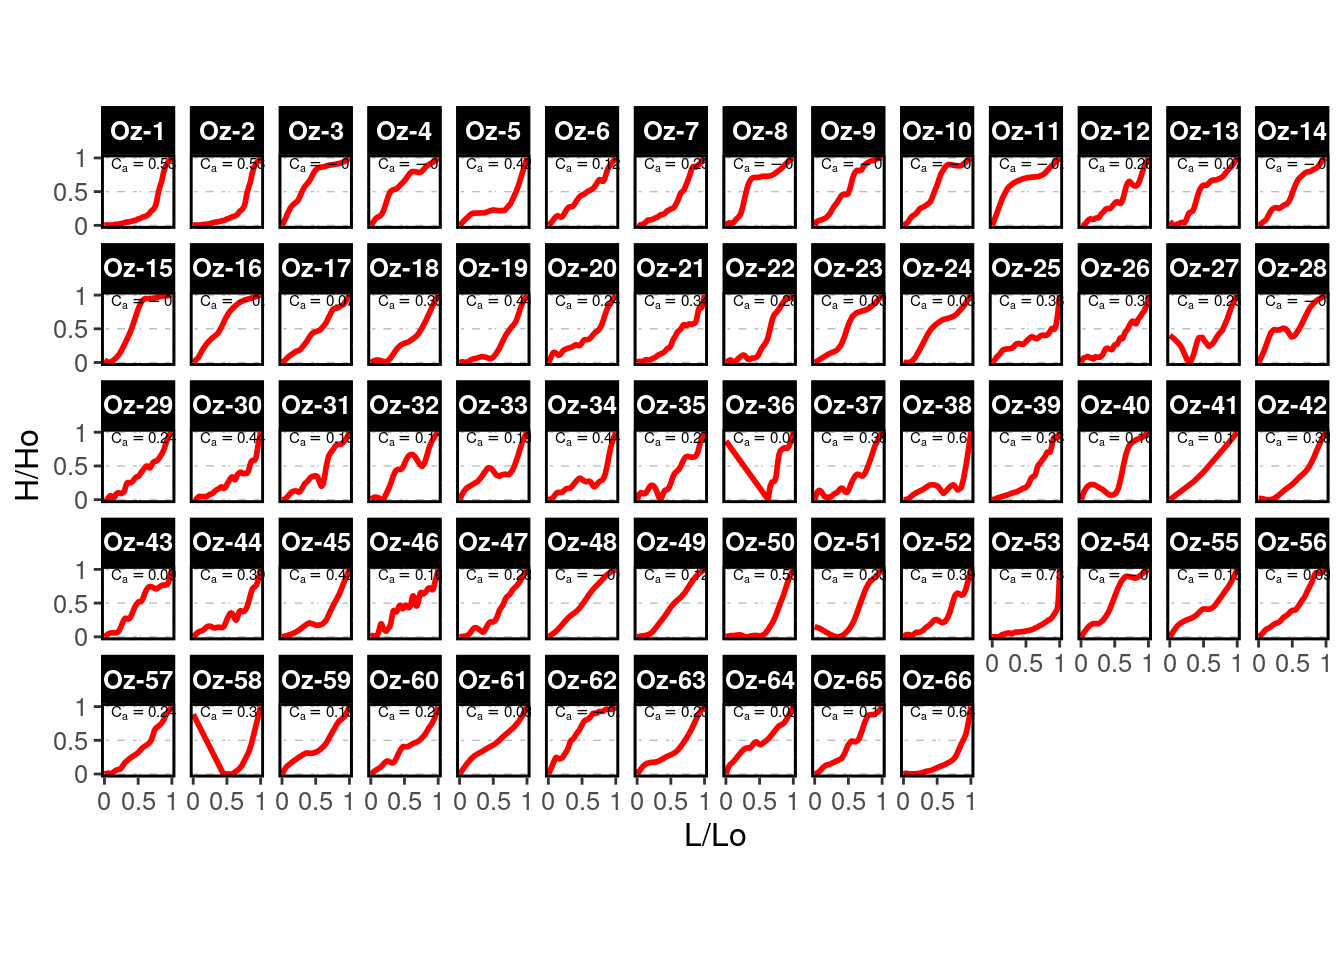
\includegraphics[width=1.00000\textwidth]{Productos Generados/p_c_yabacao.png}
\caption{\label{fig:LFP_yabacao1} Perfiles Longitudinales e Indices de
Concavidad de la subcuenta Rio Yabacao}
\end{figure}

\begin{figure}
\centering
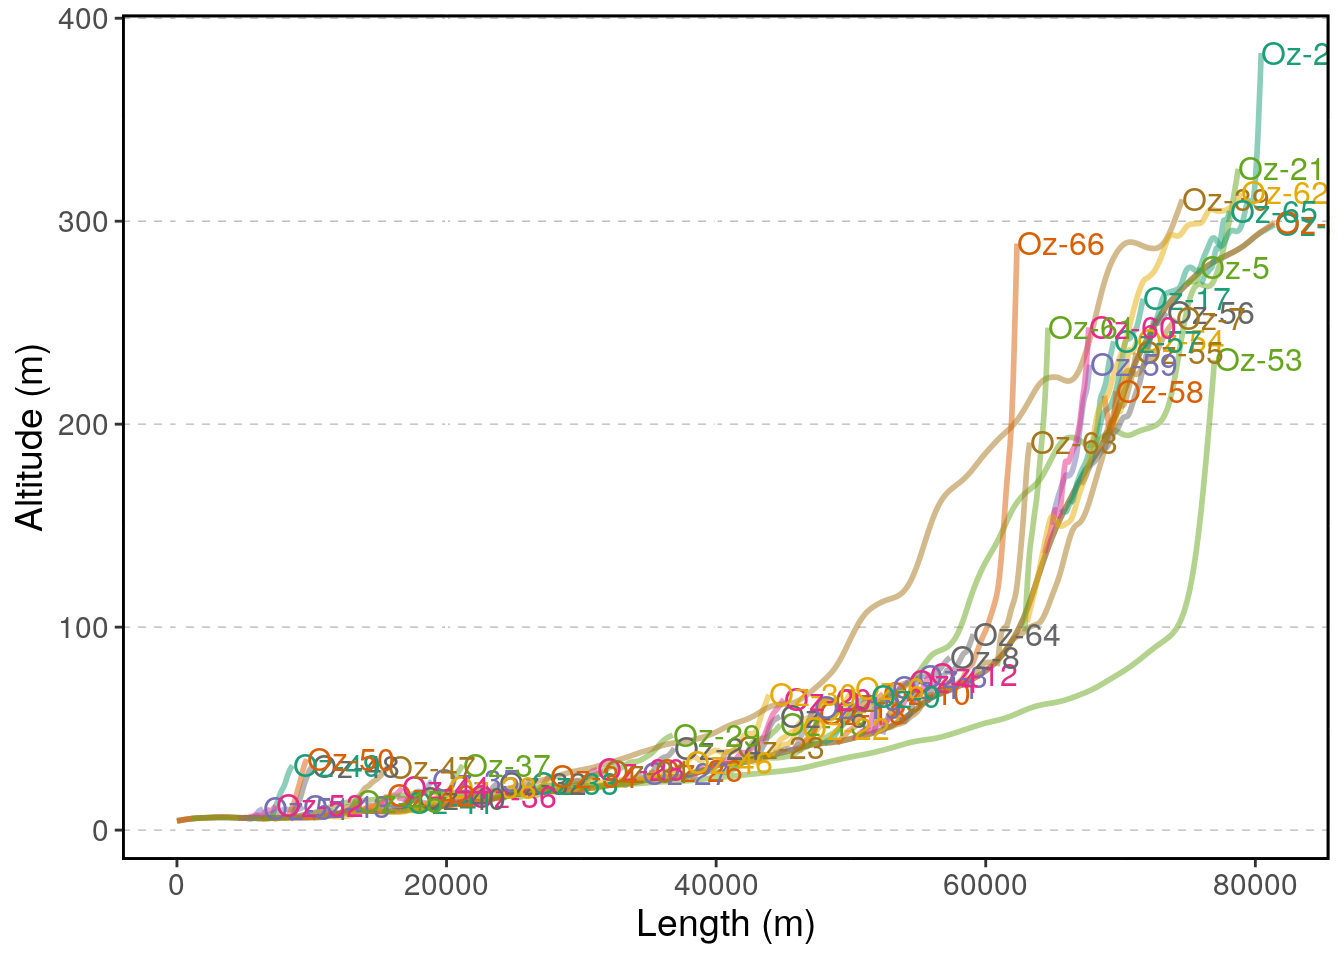
\includegraphics[width=0.75000\textwidth]{Productos Generados/p_c_yabacao_todos.png}
\caption{\label{fig:LFP_yabacao2} Todos los Perfiles de elevación de la
subcuenta principal Rio Yabacao}
\end{figure}

\newpage

\subsubsection{Subcuenca Arroyo Ocoa}\label{subcuenca-arroyo-ocoa}

Los perfiles LFP que drenan el Arroyo Ocoa muestran un patrón rectilíneo
predominante. Presentan claramente tres patrones, uno formado por
perfiles convexos con meseta en cabecera, perfiles rectilíneos y una
gran cantidad de sifones.(Ver figura \ref{fig:LFP_ocoa0},
\ref{fig:LFP_ocoa1} y \ref{fig:LFP_ocoa2}).

\begin{figure}
\centering
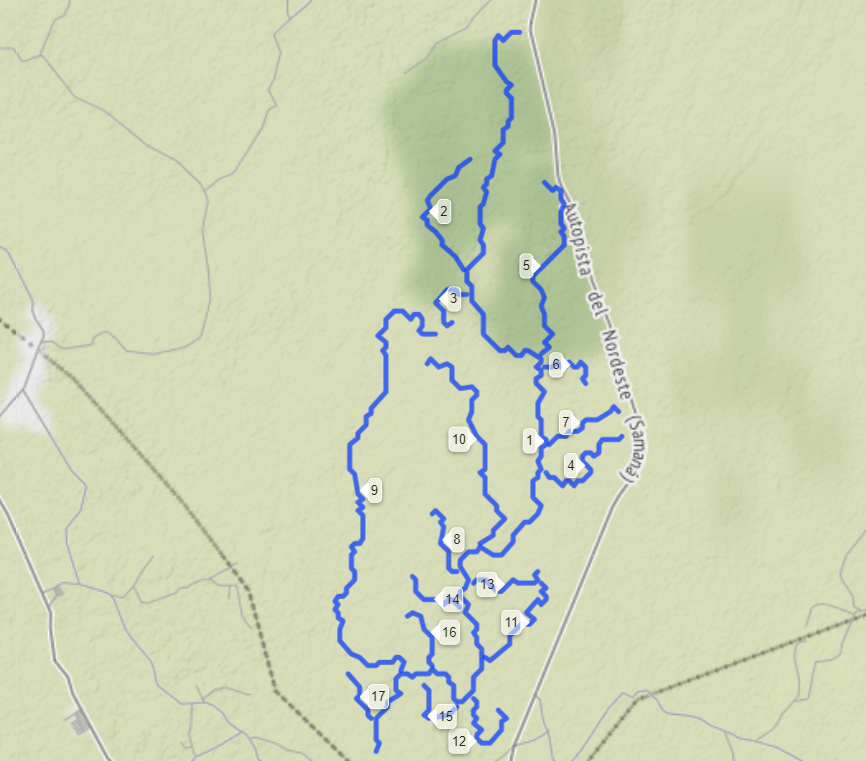
\includegraphics[width=0.60000\textwidth]{Productos Generados/p_Ocoa.png}
\caption{\label{fig:LFP_ocoa0} Subcuenta Arroyo Ocoa}
\end{figure}

\begin{figure}
\centering
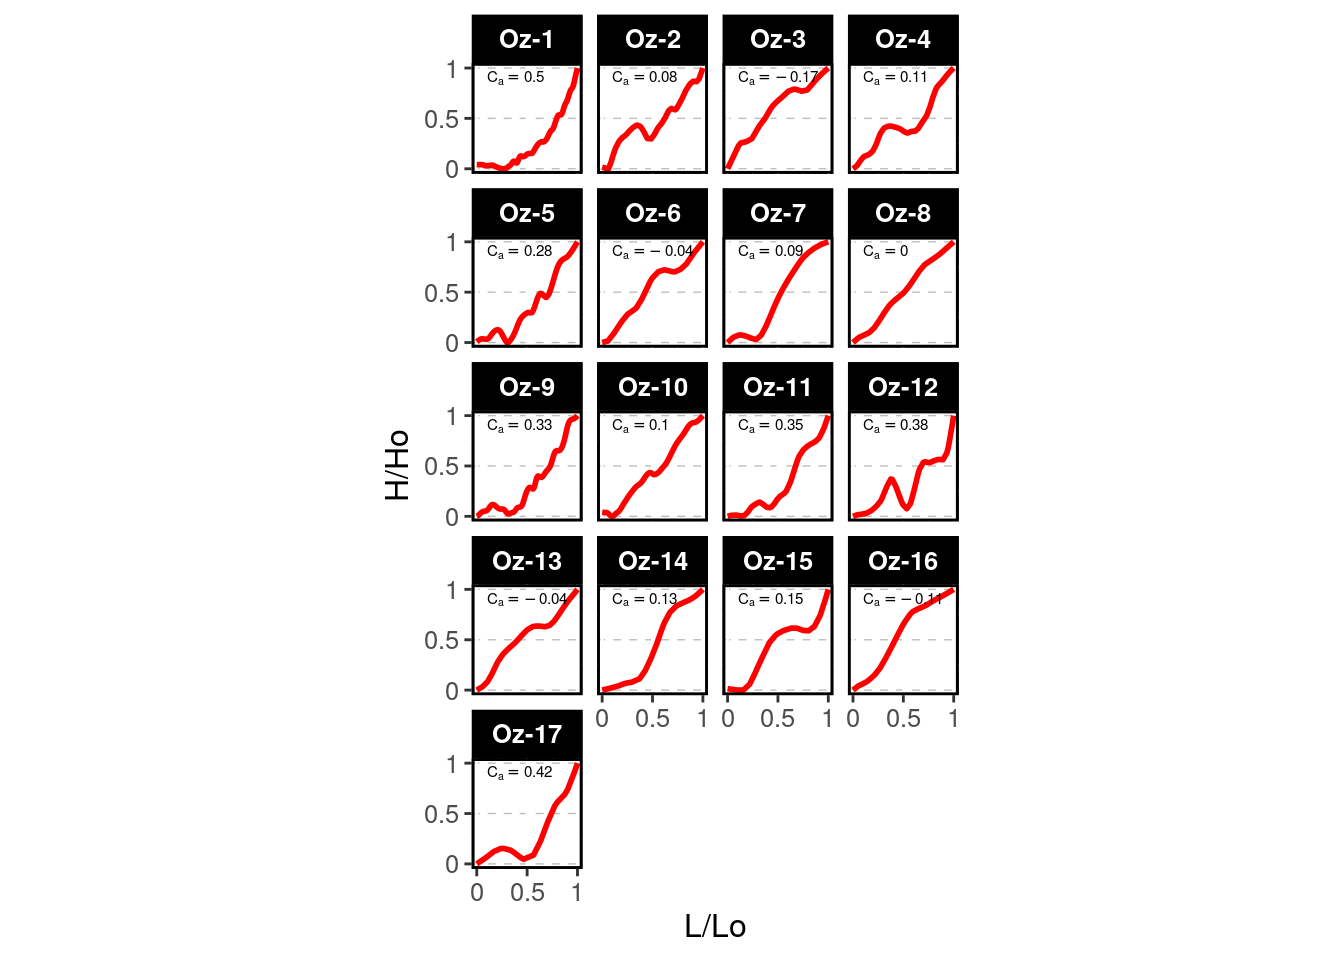
\includegraphics[width=0.85000\textwidth]{Productos Generados/p_c_ocoa1.png}
\caption{\label{fig:LFP_ocoa1} Perfiles Longitudinales e Indices de
Concavidad de la subcuenta Arroyo Ocoa}
\end{figure}

\begin{figure}
\centering
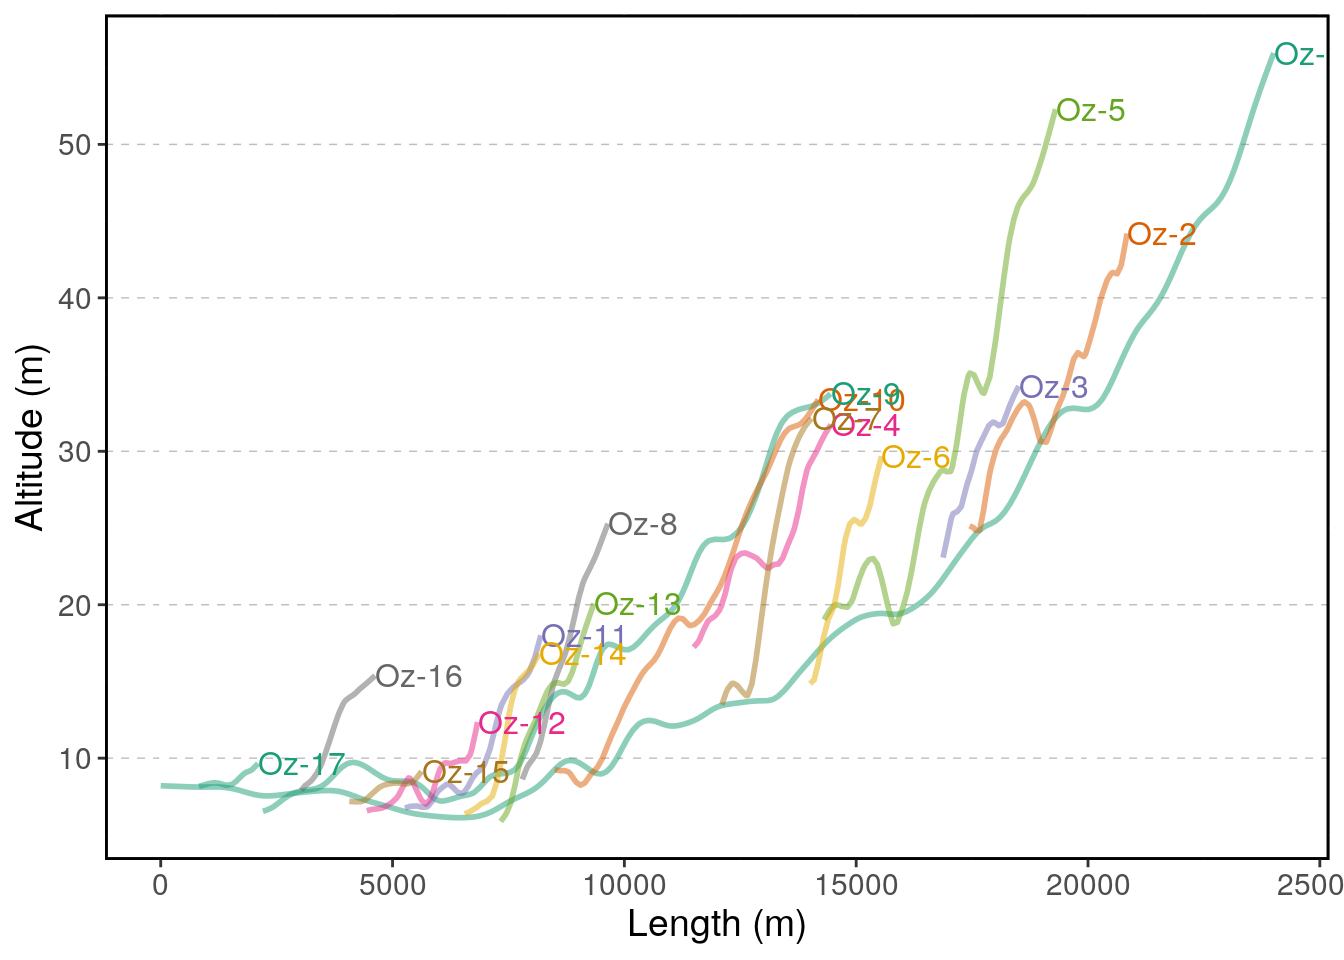
\includegraphics[width=0.75000\textwidth]{Productos Generados/p_c_ocoa.png}
\caption{\label{fig:LFP_ocoa2} Todos los Perfiles de elevación de la
subcuenca Arroyo Ocoa}
\end{figure}

\subsubsection{Subcuenca Rio La Savita}\label{subcuenca-rio-la-savita}

Con altura máxima de aproximadamente 500 metros, la subcuenca Rio La
Savita, posee perfiles longitudinales cóncavos predominantes, así como
perfiles de concavidad perfecta y en cantidades muy mínimas presenta
sifones y mesetas en cabeceras. (Ver figura \ref{fig:LFP_Savita0},
\ref{fig:LFP_Savita1} y \ref{fig:LFP_Savita2}).

\begin{figure}
\centering
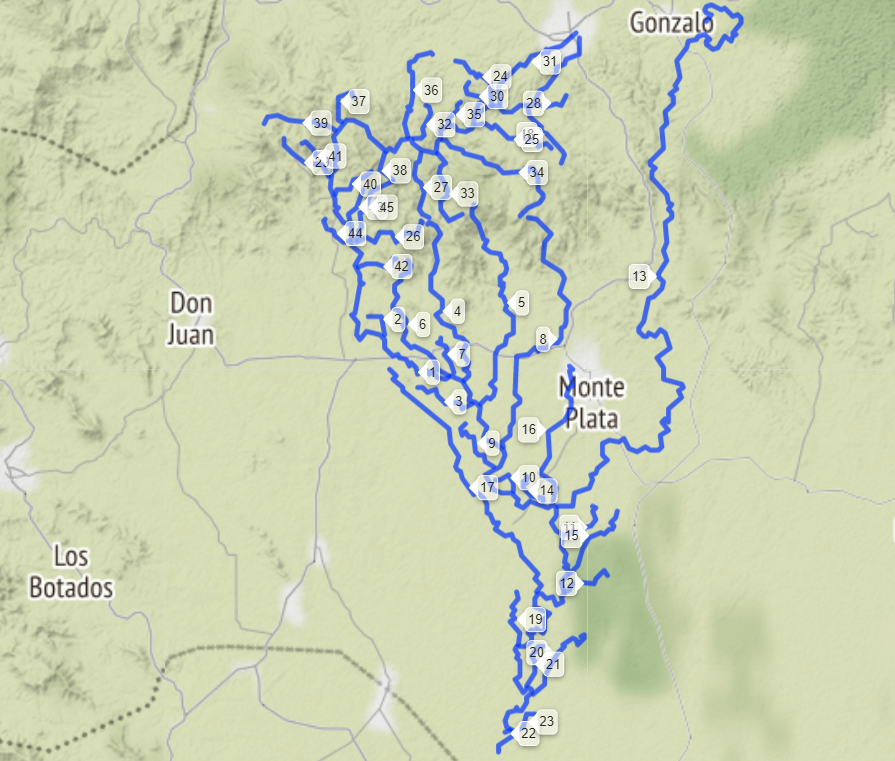
\includegraphics[width=0.65000\textwidth]{Productos Generados/p_Savita.png}
\caption{\label{fig:LFP_Savita0} Subcuenta Rio La Savita}
\end{figure}

\begin{figure}
\centering
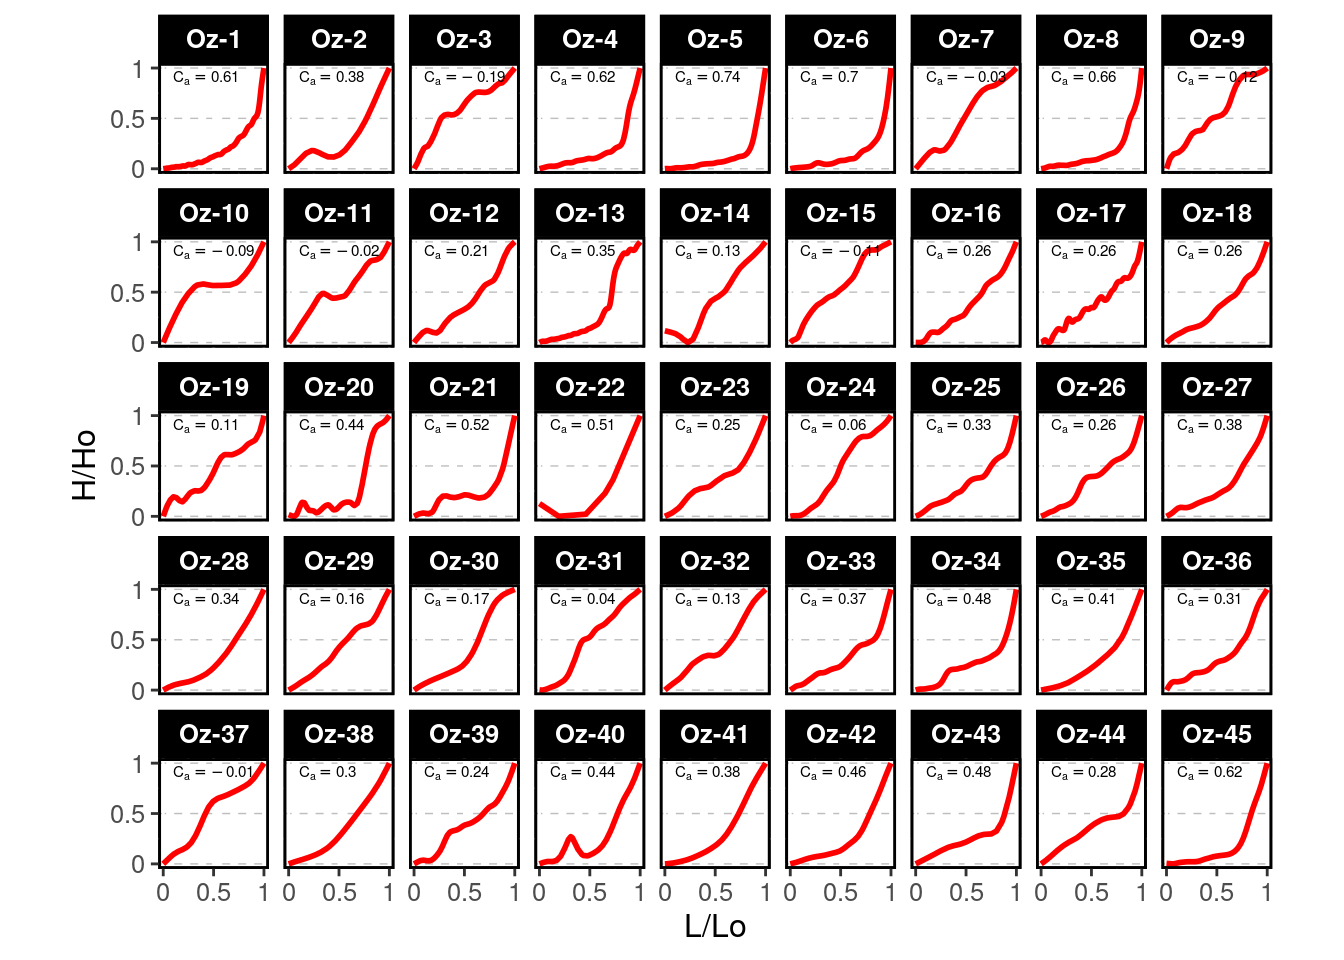
\includegraphics[width=0.75000\textwidth]{Productos Generados/p_c_savita1.png}
\caption{\label{fig:LFP_Savita1} Perfiles Longitudinales e Indices de
Concavidad de la subcuenta Rio La Savita}
\end{figure}

\begin{figure}
\centering
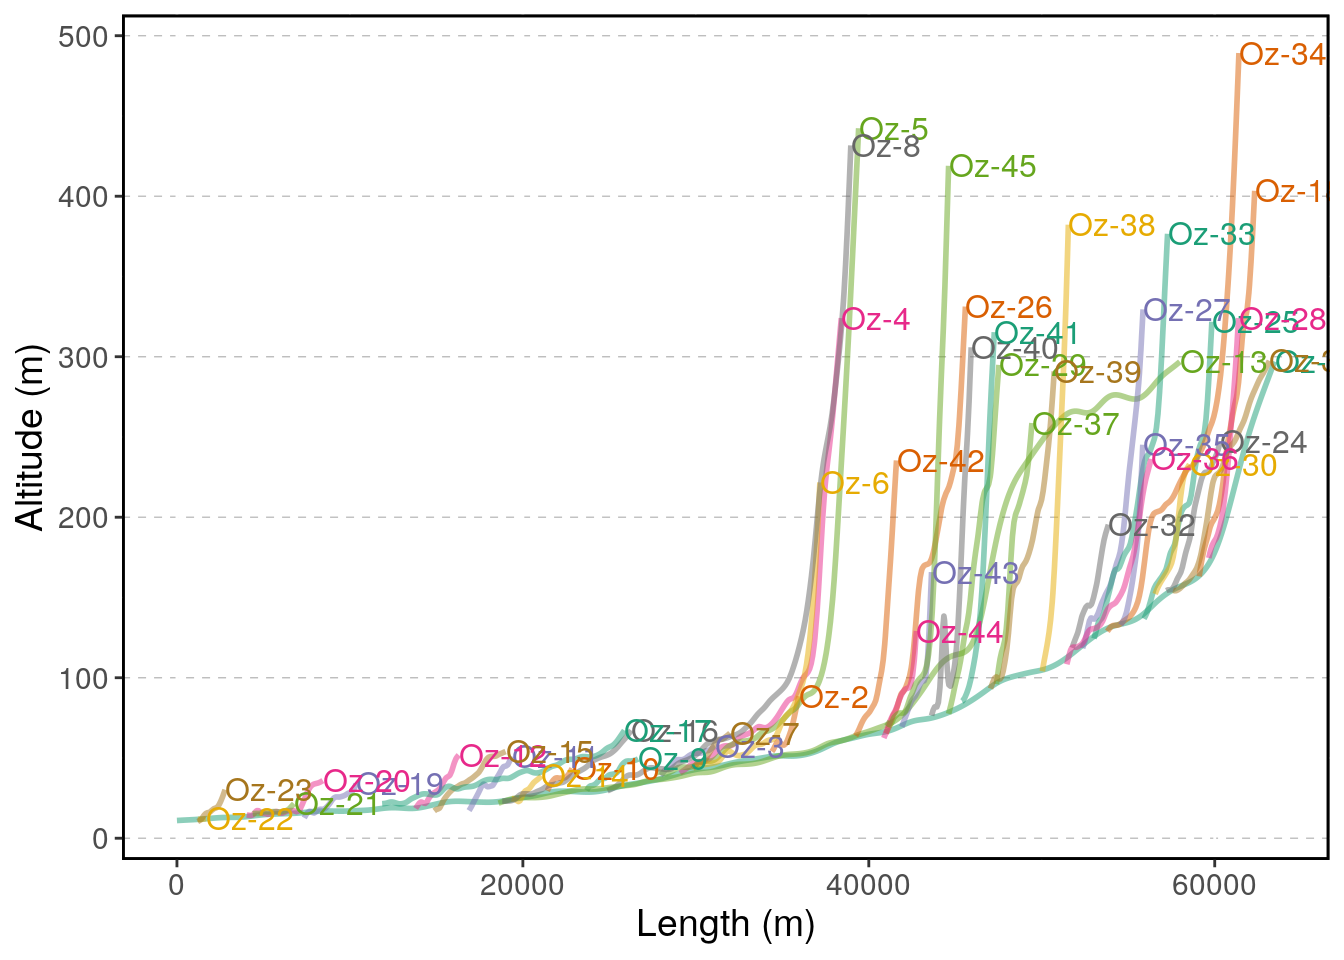
\includegraphics[width=0.75000\textwidth]{Productos Generados/p_c_savita.png}
\caption{\label{fig:LFP_Savita2} Todos los Perfiles de elevación de la
subcuenta principal Rio Savita}
\end{figure}

\subsubsection{Subcuenca Arroyo Yuca}\label{subcuenca-arroyo-yuca}

Los perfiles longitudinales que drenan el Arroyo Yuca presentan dos
grupos de patrones, el cóncavo y el rectilíneo. Destacándose más los
perfiles cóncavos.(Ver figura \ref{fig:LFP_Yuca0}, \ref{fig:LFP_Yuca1} y
\ref{fig:LFP_Yuca2}).

\begin{figure}
\centering
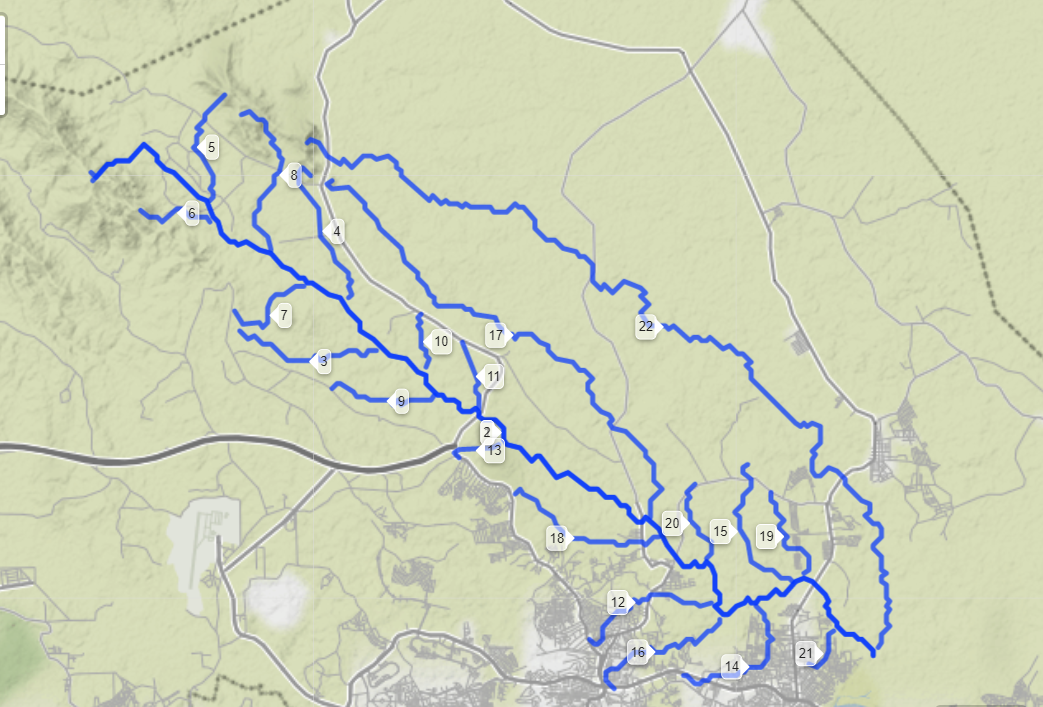
\includegraphics[width=0.65000\textwidth]{Productos Generados/p_yuca.png}
\caption{\label{fig:LFP_Yuca0} Subcuenta Arroyo Yuca}
\end{figure}

\begin{figure}
\centering
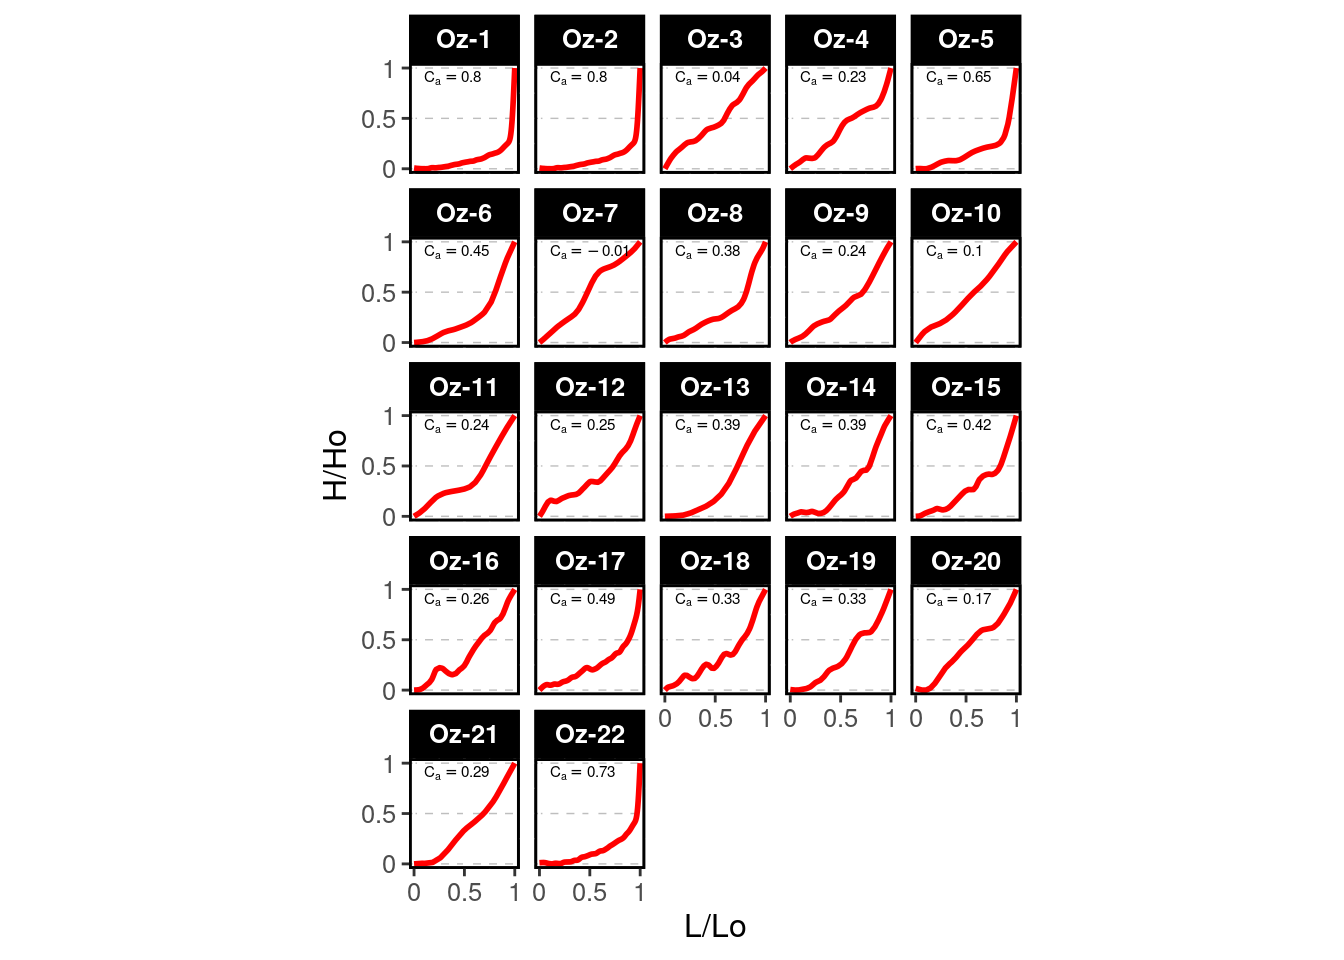
\includegraphics[width=0.75000\textwidth]{Productos Generados/p_c_yuca1.png}
\caption{\label{fig:LFP_Yuca1} Perfiles Longitudinales e Indices de
Concavidad de la subcuenta Arroyo Yuca}
\end{figure}

\begin{figure}
\centering
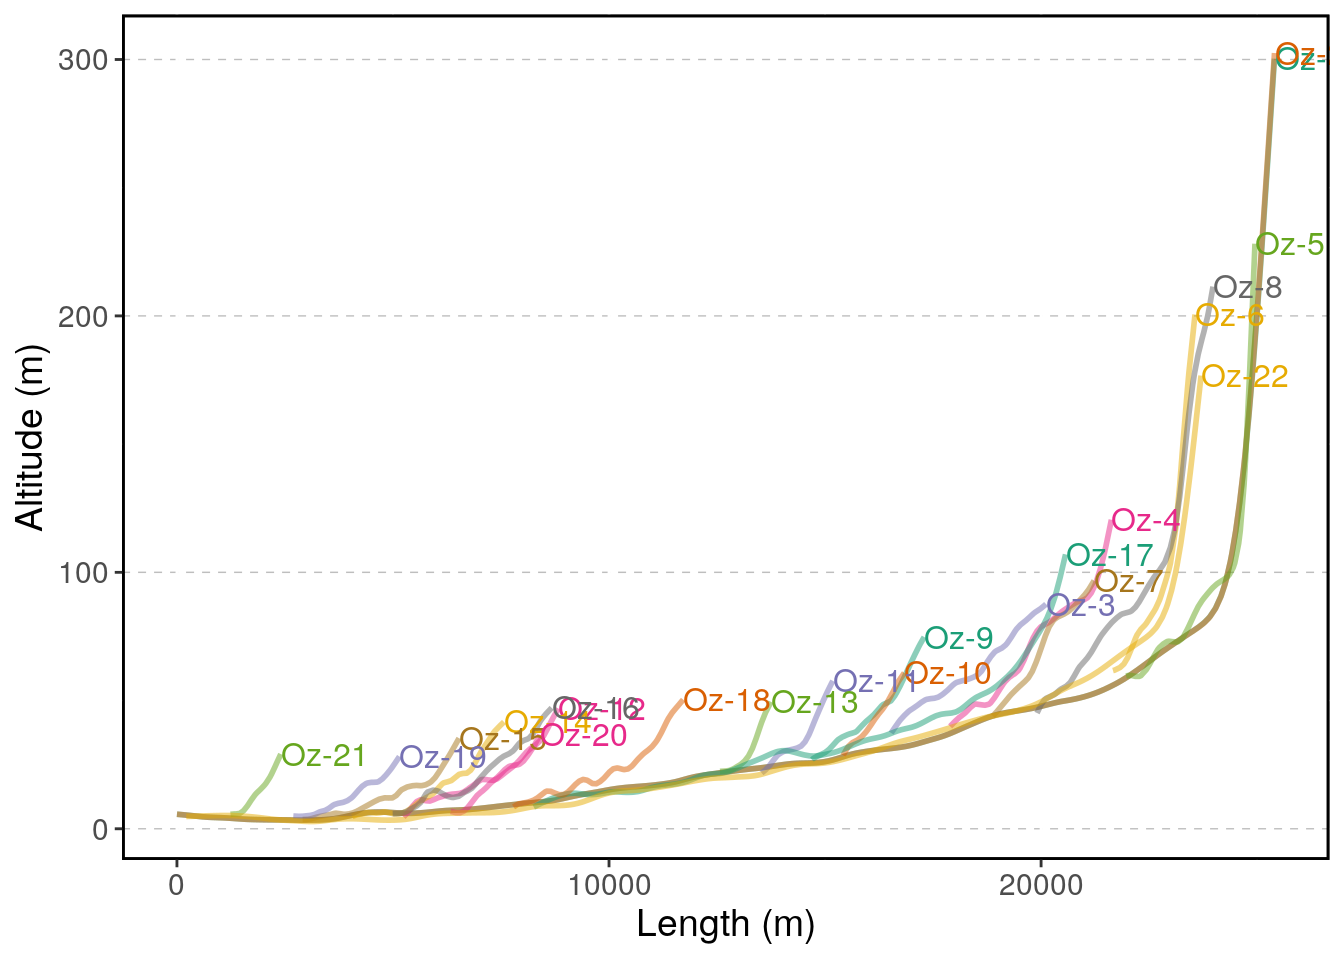
\includegraphics[width=0.75000\textwidth]{Productos Generados/p_c_yuca.png}
\caption{\label{fig:LFP_Yuca2} Todos los Perfiles de elevación de la
subcuenta Arroyo Yuca}
\end{figure}

\subsubsection{Subcuenca Rio Isabela}\label{subcuenca-rio-isabela}

Los perfiles cóncavos están muy presentes en la sucuenca del Rio
Isabela, evidencia de esto, es la presencia de una gran cantidad de
perfiles cóncavos perfectos, sim embargo también presentan un grupo de
valores de índices de concavidad negativos dando origen a mesetas en
cabeceras poco pronunciadas.(Ver figura \ref{fig:LFP_Isabela0},
\ref{fig:LFP_Isabela1} y \ref{fig:LFP_Isabela2}).

\begin{figure}
\centering
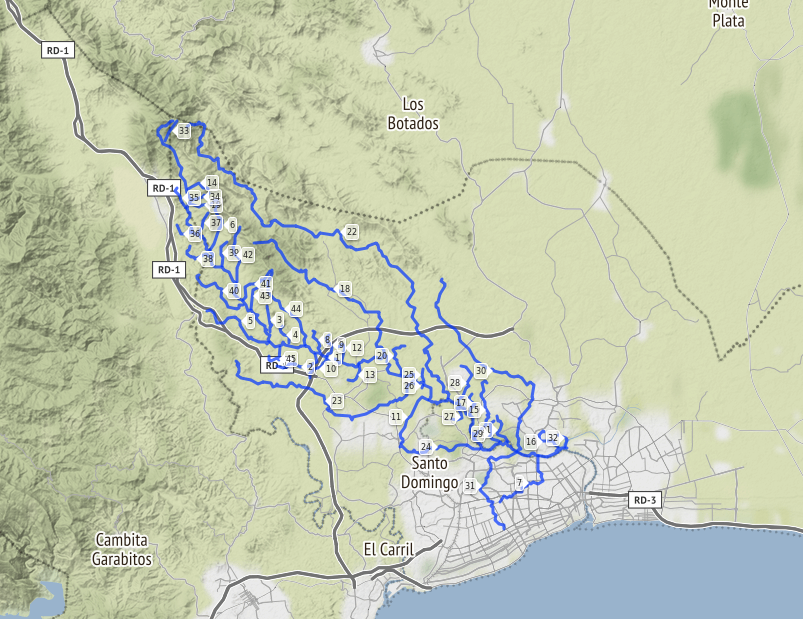
\includegraphics[width=0.65000\textwidth]{Productos Generados/p_isabela.png}
\caption{\label{fig:LFP_Isabela0} Subcuenta Rio Isabela}
\end{figure}

\begin{figure}
\centering
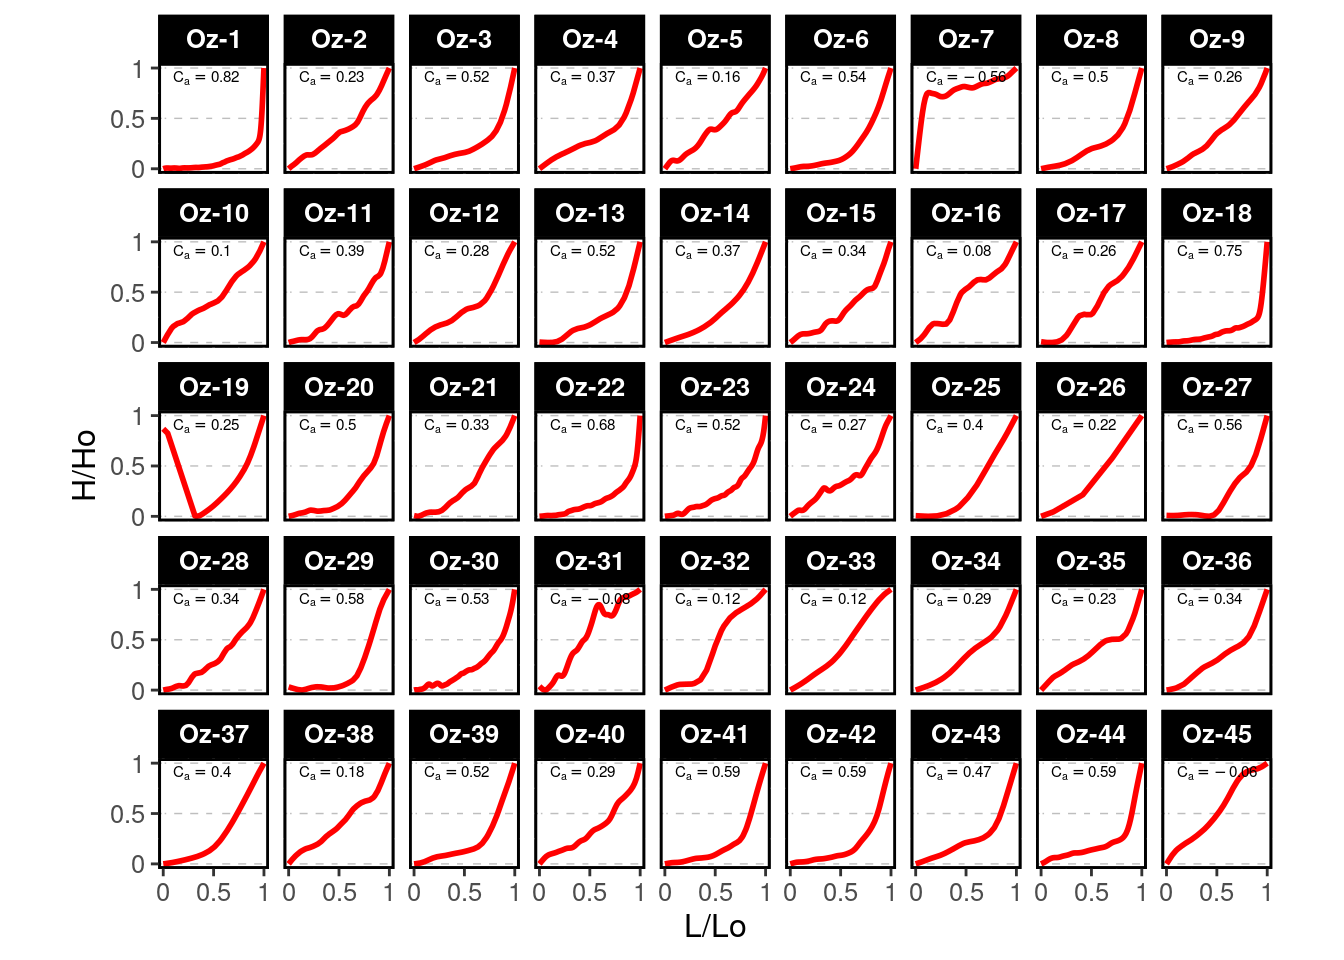
\includegraphics[width=0.75000\textwidth]{Productos Generados/p_c_isabela1.png}
\caption{\label{fig:LFP_Isabela1} Perfiles Longitudinales e Indices de
Concavidad de la subcuenta Rio Isabela}
\end{figure}

\begin{figure}
\centering
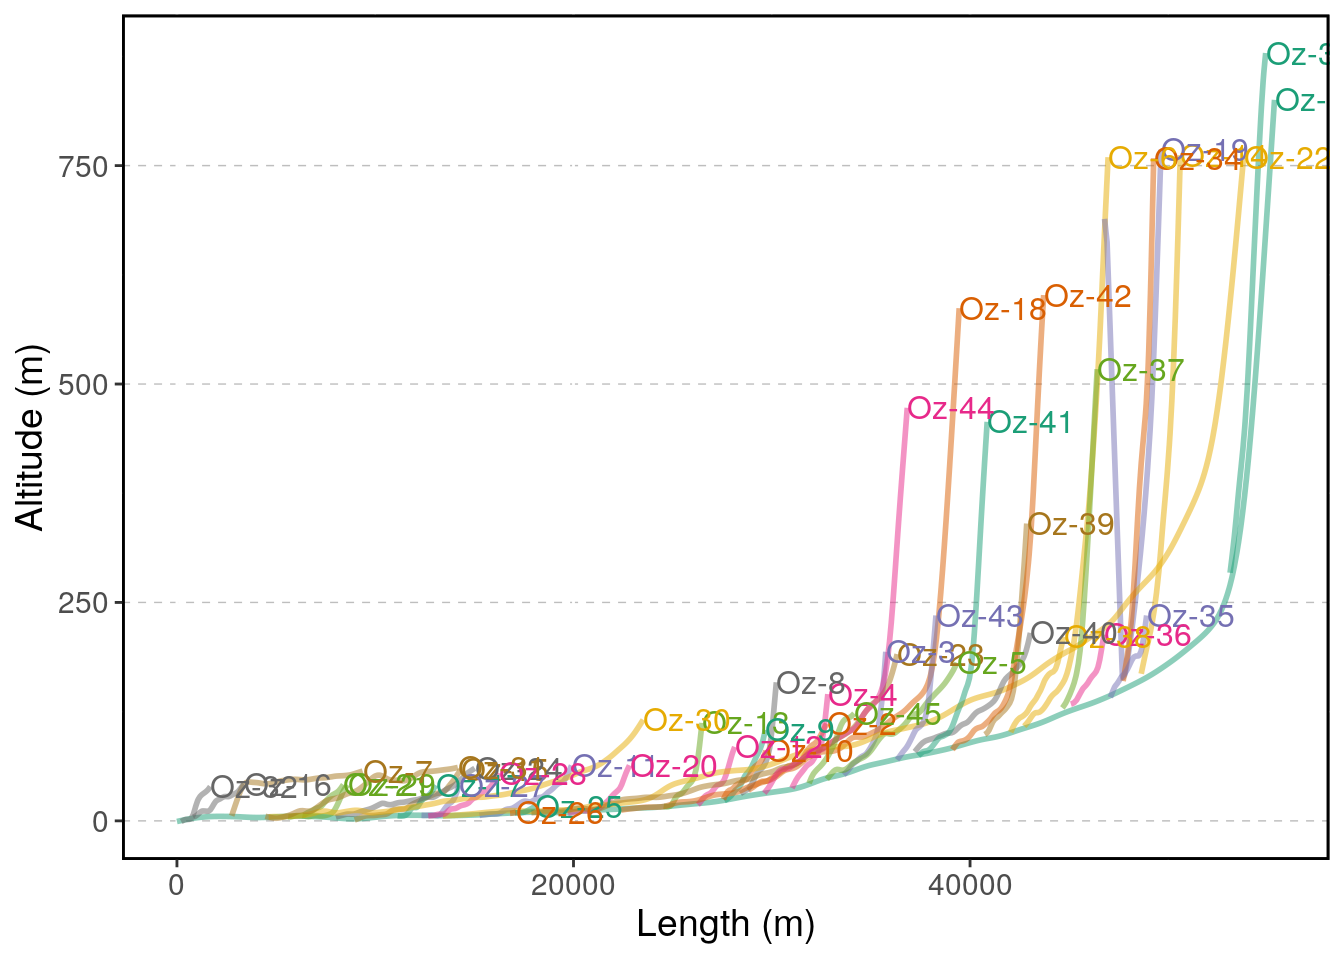
\includegraphics[width=0.75000\textwidth]{Productos Generados/p_c_isabela.png}
\caption{\label{fig:LFP_Isabela2} Todos los Perfiles de elevación de la
subcuenta Rio Isabela}
\end{figure}

\newpage

\subsection{Curso mas largo de la
cuenca}\label{curso-mas-largo-de-la-cuenca}

Loma Rancho de Yagua-Loma Palo Bonito, allí nace el Ozama, o al menos
allí se enraíza su curso más largo, desembocando en el Mar Caribe (Ver
figura \ref{fig:c_m_l}).

\begin{figure}
\centering
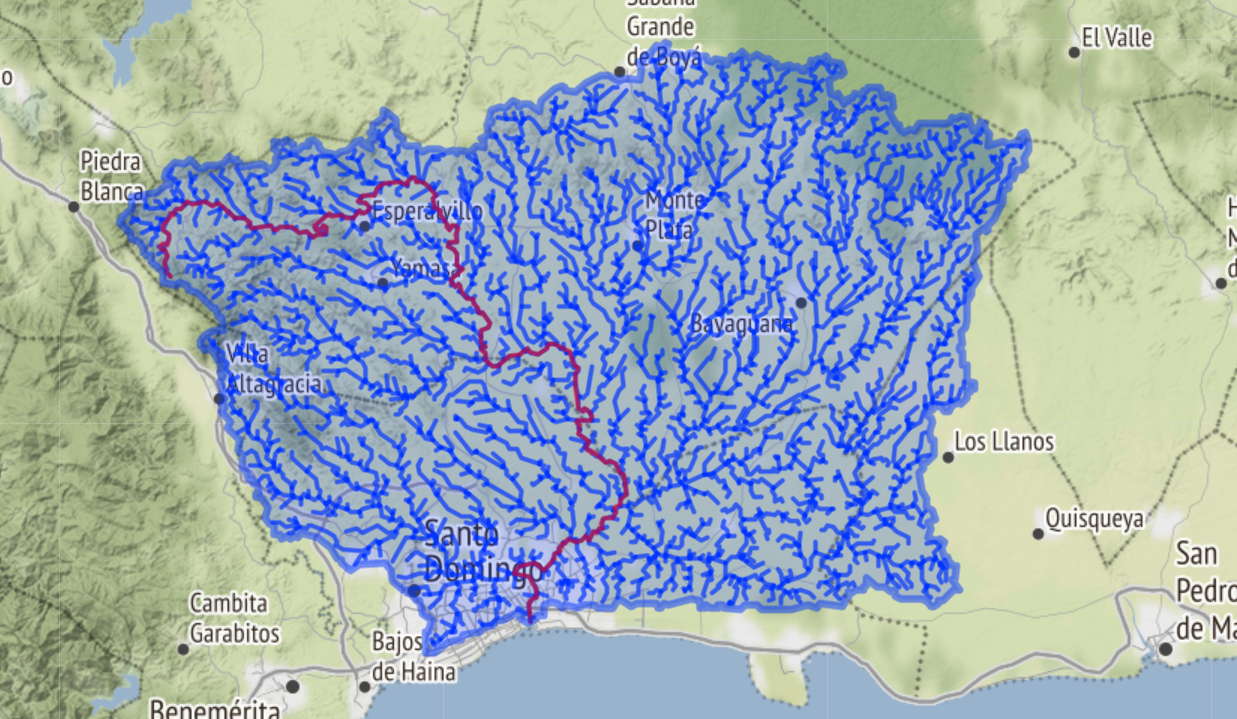
\includegraphics[width=0.75000\textwidth]{Productos Generados/curso mas largo.png}
\caption{\label{fig:c_m_l} Curso mas largo de la cuenca Ozama}
\end{figure}

\newpage

\section{Discusión}\label{discusiuxf3n}

A partir de los hallazgos encontrados, se observa de manera visual dos
posibles codos de captura, a) Uno ubicada al este de Piedra y al norte
de Esperalvillo, existiendo probabilidad de que el curso fluvial más
largo del Ozama drenara sus aguas hacia los Haitises; b) el segundo es
el En curso fluvial que sale de Sabana Grande de Boya hacia el Rio
Ozama, pudiendo este en el pasado drenar sus aguas en el Rio Camú, o en
algún otro rio del noreste de la Isla de Santo Domingo.

Al superponer la Cuenca Ozama generada con el Mapa Geológico Nacional,
en las zonas donde están estos posibles codos de capturas, predominan
las rocas clásticas y las rocas calizas, por lo que, se planeta la
posible existencia de piratería kárstica en estas zonas.

Esta hipótesis se relaciona con lo planteado por Jose Ramon Martinez
Batlle (2019), quien señala que la piratería kárstica es un motor
potencial del reordenamiento del drenaje, y que ocurre en zonas de
afloramiento de piedras calizas. De igual manera también se relaciona
con lo establecido por Gutiérrez Elorza (2008) , quien explica que si la
roca se erosiona fácilmente, como marga o arcilla, se produce una rápida
erosión que puede provocar la división de un río, para finalmente
producir una captura por otro rio.

La caracterización morfológica de la red de drenaje de la Cuenca Ozama,
presenta cuatro patrones de redes de drenaje bien definidos (Paralela,
Rectangular, Dendrítica, Enrejada), esto según Gutiérrez Elorza (2008)
es debido a la interacción fluvial con los materiales erosionables,
argumento que pudimos comprobar, al observar (en el mapa Geológico
Nacional) que la cuenca drena sus aguas a través de una diversidad de
rocas.

Si el clima y la litología permanecen sin cambios, la razón de
bifurcación (Rb) explicada por el resultado de la relación entre el
número de cauces de cualquier orden y el número de cauces en el orden
inferior, dicho resultado siempre será constante entre un orden y otro
(Horton, 1945). Las razones de bifurcación calculada para los pares de
órdenes de red 4-5, y 5-6, de la Cuenca Ozama no se ajustan al criterio
planteado por Horton, debido a que estas varían con valores que van
desde 1 a 2. La guía elaborada por Martínez Batlle (2020) explica que la
razón de bifurcación calculada por los métodos de coeficientes de
regresión y por el promedio de las razones de bifurcación de cada par de
órdenes de red, difieren en sus resultados, esto fue comprobado para la
razón de bifurcación calculada a la Cuenca Ozama por ambos métodos, sin
embargo el error resultante es un valor muy pequeño.

\section{\texorpdfstring{\emph{Script}
reproducible}{Script reproducible}}\label{script-reproducible}

\subsection{Paquetes}\label{paquetes}

\begin{Shaded}
\begin{Highlighting}[]
\KeywordTok{library}\NormalTok{(rgrass7)}
\end{Highlighting}
\end{Shaded}

\subsection{Región de GRASS}\label{regiuxf3n-de-grass}

\begin{Shaded}
\begin{Highlighting}[]
\NormalTok{gisdbase <-}\StringTok{ 'grass-data-test'} \CommentTok{#Base de datos de GRASS GIS}
\NormalTok{wd <-}\StringTok{ }\KeywordTok{getwd}\NormalTok{() }\CommentTok{#Directorio de trabajo}
\NormalTok{wd}
\NormalTok{loc <-}\StringTok{ }\KeywordTok{initGRASS}\NormalTok{(}\DataTypeTok{gisBase =} \StringTok{"/usr/lib/grass78/"}\NormalTok{,}
                 \DataTypeTok{home =}\NormalTok{ wd,}
                 \DataTypeTok{gisDbase =} \KeywordTok{paste}\NormalTok{(wd, gisdbase, }\DataTypeTok{sep =} \StringTok{'/'}\NormalTok{),}
                 \DataTypeTok{location =} \StringTok{'rdom'}\NormalTok{,}
                 \DataTypeTok{mapset =} \StringTok{"PERMANENT"}\NormalTok{,}
                 \DataTypeTok{override =} \OtherTok{TRUE}\NormalTok{)}
\end{Highlighting}
\end{Shaded}

\begin{Shaded}
\begin{Highlighting}[]
\NormalTok{knitr}\OperatorTok{::}\NormalTok{opts_chunk}\OperatorTok{$}\KeywordTok{set}\NormalTok{(}
  \DataTypeTok{echo =} \OtherTok{TRUE}\NormalTok{,}
  \DataTypeTok{collapse=}\OtherTok{TRUE}\NormalTok{,}
  \DataTypeTok{eval =}\NormalTok{ T}
\NormalTok{)}
\end{Highlighting}
\end{Shaded}

\begin{Shaded}
\begin{Highlighting}[]
\KeywordTok{source}\NormalTok{(}
\NormalTok{  knitr}\OperatorTok{::}\KeywordTok{purl}\NormalTok{(}
    \StringTok{'intro-rgrass.Rmd'}\NormalTok{,}
    \DataTypeTok{output=}\KeywordTok{tempfile}\NormalTok{()}
\NormalTok{  )}
\NormalTok{)}
\end{Highlighting}
\end{Shaded}

\subsection{Proceso 0}\label{proceso-0}

\begin{Shaded}
\begin{Highlighting}[]
\CommentTok{#Quité el paquete rgrass7, porque ya se carga al ejecutar el script intro-rgrass.Rmd}
\KeywordTok{library}\NormalTok{(sf)}
\KeywordTok{library}\NormalTok{(raster)}
\KeywordTok{library}\NormalTok{(sp)}
\end{Highlighting}
\end{Shaded}

\subsection{Definir proyección basado en una fuente externa, en este
caso, el DEM
MERIT}\label{definir-proyecciuxf3n-basado-en-una-fuente-externa-en-este-caso-el-dem-merit}

\begin{Shaded}
\begin{Highlighting}[]
\KeywordTok{gmeta}\NormalTok{()}
\NormalTok{dem <-}\StringTok{ 'data/dem.tif'}
\CommentTok{#Definir la proyección de la región basada en DEM}
\KeywordTok{execGRASS}\NormalTok{(}
  \DataTypeTok{cmd =} \StringTok{'g.proj'}\NormalTok{,}
  \DataTypeTok{flags =} \KeywordTok{c}\NormalTok{(}\StringTok{'t'}\NormalTok{,}\StringTok{'c'}\NormalTok{),}
  \DataTypeTok{georef=}\NormalTok{dem)}
\KeywordTok{gmeta}\NormalTok{()}
\end{Highlighting}
\end{Shaded}

\subsection{Importar mapa raster}\label{importar-mapa-raster}

\begin{Shaded}
\begin{Highlighting}[]
\KeywordTok{execGRASS}\NormalTok{(}
  \DataTypeTok{cmd =} \StringTok{'r.in.gdal'}\NormalTok{,}
  \DataTypeTok{flags=}\KeywordTok{c}\NormalTok{(}\StringTok{'overwrite'}\NormalTok{,}\StringTok{'quiet'}\NormalTok{),}
  \DataTypeTok{parameters=}\KeywordTok{list}\NormalTok{(}
    \DataTypeTok{input=}\NormalTok{dem,}
    \DataTypeTok{output=}\StringTok{'dem'}
\NormalTok{  )}
\NormalTok{)}
\end{Highlighting}
\end{Shaded}

\subsection{Actualizar la extensión de la región al DEM, sólo por
precaución}\label{actualizar-la-extensiuxf3n-de-la-regiuxf3n-al-dem-suxf3lo-por-precauciuxf3n}

\begin{Shaded}
\begin{Highlighting}[]
\KeywordTok{execGRASS}\NormalTok{(}
  \DataTypeTok{cmd =} \StringTok{'g.region'}\NormalTok{,}
  \DataTypeTok{parameters=}\KeywordTok{list}\NormalTok{(}
    \DataTypeTok{raster =} \StringTok{'dem'}\NormalTok{,}
    \DataTypeTok{align =} \StringTok{'dem'}
\NormalTok{  )}
\NormalTok{)}
\end{Highlighting}
\end{Shaded}

\subsection{Mostrar la definición de la
región}\label{mostrar-la-definiciuxf3n-de-la-regiuxf3n}

\begin{Shaded}
\begin{Highlighting}[]
\KeywordTok{gmeta}\NormalTok{()}
\end{Highlighting}
\end{Shaded}

\subsection{Para completar, importar un mapa vectorial
también}\label{para-completar-importar-un-mapa-vectorial-tambiuxe9n}

\begin{Shaded}
\begin{Highlighting}[]
\NormalTok{demext <-}\StringTok{ 'data/dem-extension.geojson'}
\KeywordTok{execGRASS}\NormalTok{(}
  \DataTypeTok{cmd =} \StringTok{'v.in.ogr'}\NormalTok{,}
  \DataTypeTok{flags=}\KeywordTok{c}\NormalTok{(}\StringTok{'overwrite'}\NormalTok{,}\StringTok{'quiet'}\NormalTok{),}
  \DataTypeTok{parameters=}\KeywordTok{list}\NormalTok{(}
    \DataTypeTok{input=}\NormalTok{demext,}
    \DataTypeTok{output=}\StringTok{'dem_extent'}
\NormalTok{  )}
\NormalTok{)}

\KeywordTok{execGRASS}\NormalTok{(}
  \StringTok{'g.list'}\NormalTok{,}
  \DataTypeTok{flags =} \StringTok{'t'}\NormalTok{,}
  \DataTypeTok{parameters =} \KeywordTok{list}\NormalTok{(}
    \DataTypeTok{type =} \KeywordTok{c}\NormalTok{(}\StringTok{'raster'}\NormalTok{, }\StringTok{'vector'}\NormalTok{)}
\NormalTok{  )}
\NormalTok{)}

\KeywordTok{source}\NormalTok{(}\StringTok{'borrar_mascara_si_la_hubiere.R'}\NormalTok{)}
\KeywordTok{unlink_.gislock}\NormalTok{()}
\end{Highlighting}
\end{Shaded}

\section{\texorpdfstring{title: ``Calcular parámetros hidrográficos con
r.watershed. Visualizar con
leaflet''}{title: Calcular parámetros hidrográficos con r.watershed. Visualizar con leaflet}}\label{title-calcular-paruxe1metros-hidrogruxe1ficos-con-r.watershed.-visualizar-con-leaflet}

\begin{Shaded}
\begin{Highlighting}[]
\NormalTok{knitr}\OperatorTok{::}\NormalTok{opts_chunk}\OperatorTok{$}\KeywordTok{set}\NormalTok{(}
  \DataTypeTok{echo =} \OtherTok{TRUE}\NormalTok{,}
  \DataTypeTok{collapse=}\OtherTok{TRUE}\NormalTok{,}
  \DataTypeTok{eval =}\NormalTok{ T}
\NormalTok{)}
\KeywordTok{options}\NormalTok{(}\DataTypeTok{knitr.duplicate.label =} \StringTok{"allow"}\NormalTok{)}
\end{Highlighting}
\end{Shaded}

\subsection{ejecutar Scrit anteriores}\label{ejecutar-scrit-anteriores}

\begin{Shaded}
\begin{Highlighting}[]
\KeywordTok{source}\NormalTok{(}
\NormalTok{  knitr}\OperatorTok{::}\KeywordTok{purl}\NormalTok{(}
    \StringTok{'proyeccion-importar-fuente-extension_C_Propia.Rmd'}\NormalTok{,}
    \DataTypeTok{output=}\KeywordTok{tempfile}\NormalTok{()}
\NormalTok{  )}
\NormalTok{)}
\NormalTok{knitr}\OperatorTok{::}\NormalTok{opts_chunk}\OperatorTok{$}\KeywordTok{set}\NormalTok{(}\DataTypeTok{fig.path =} \StringTok{"img/calcwshed/"}\NormalTok{)}
\end{Highlighting}
\end{Shaded}

\subsection{\texorpdfstring{\texttt{g.list}}{g.list}}\label{g.list}

\begin{Shaded}
\begin{Highlighting}[]
\KeywordTok{execGRASS}\NormalTok{(}
  \StringTok{'g.list'}\NormalTok{,}
  \DataTypeTok{flags =} \StringTok{'t'}\NormalTok{,}
  \DataTypeTok{parameters =} \KeywordTok{list}\NormalTok{(}
    \DataTypeTok{type =} \KeywordTok{c}\NormalTok{(}\StringTok{'raster'}\NormalTok{, }\StringTok{'vector'}\NormalTok{)}
\NormalTok{  )}
\NormalTok{)}
\end{Highlighting}
\end{Shaded}

\subsection{\texorpdfstring{Calcular parámetros hidrográficos de interés
usando
\texttt{r.watershed}}{Calcular parámetros hidrográficos de interés usando r.watershed}}\label{calcular-paruxe1metros-hidrogruxe1ficos-de-interuxe9s-usando-r.watershed}

\begin{Shaded}
\begin{Highlighting}[]
\KeywordTok{execGRASS}\NormalTok{(}
  \StringTok{"r.watershed"}\NormalTok{,}
  \DataTypeTok{flags =} \KeywordTok{c}\NormalTok{(}\StringTok{'overwrite'}\NormalTok{,}\StringTok{'quiet'}\NormalTok{),}
  \DataTypeTok{parameters =} \KeywordTok{list}\NormalTok{(}
    \DataTypeTok{elevation =} \StringTok{"dem"}\NormalTok{,}
    \DataTypeTok{accumulation =} \StringTok{"accum-de-rwshed"}\NormalTok{,}
    \DataTypeTok{stream =} \StringTok{"stream-de-rwshed"}\NormalTok{,}
    \DataTypeTok{drainage =} \StringTok{"drainage-dir-de-rwshed"}\NormalTok{,}
    \DataTypeTok{basin =} \StringTok{'basins'}\NormalTok{,}
    \DataTypeTok{half_basin =} \StringTok{'half-basins'}\NormalTok{,}
    \DataTypeTok{threshold =} \DecValTok{80}
\NormalTok{  )}
\NormalTok{)}
\end{Highlighting}
\end{Shaded}

\subsection{Traer capas a R}\label{traer-capas-a-r}

\begin{Shaded}
\begin{Highlighting}[]
\CommentTok{# Usar Spatial }
\KeywordTok{library}\NormalTok{(sp)}
\KeywordTok{use_sp}\NormalTok{()}
\CommentTok{#Paquete manejo de los raster}
\KeywordTok{library}\NormalTok{(raster)}
\CommentTok{#DEM}
\NormalTok{dem <-}\StringTok{ }\KeywordTok{raster}\NormalTok{(}\KeywordTok{readRAST}\NormalTok{(}\StringTok{'dem'}\NormalTok{))}
\CommentTok{#Basins}
\NormalTok{basins <-}\StringTok{ }\KeywordTok{raster}\NormalTok{(}\KeywordTok{readRAST}\NormalTok{(}\StringTok{'basins'}\NormalTok{))}
\CommentTok{#Stream network}
\NormalTok{stream <-}\StringTok{ }\KeywordTok{raster}\NormalTok{(}\KeywordTok{readRAST}\NormalTok{(}\StringTok{'stream-de-rwshed'}\NormalTok{))}
\NormalTok{stream3857 <-}\StringTok{ }\KeywordTok{projectRaster}\NormalTok{(stream, }\DataTypeTok{crs =} \KeywordTok{CRS}\NormalTok{(}\StringTok{"+init=epsg:3857"}\NormalTok{), }\DataTypeTok{method =} \StringTok{'ngb'}\NormalTok{)}
\CommentTok{#Generar un vectorial de extensión de capa en EPSG:4326}
\NormalTok{e <-}\StringTok{ }\KeywordTok{extent}\NormalTok{(stream)}
\NormalTok{e <-}\StringTok{ }\KeywordTok{as}\NormalTok{(e, }\StringTok{'SpatialPolygons'}\NormalTok{)}
\KeywordTok{proj4string}\NormalTok{(e) <-}\StringTok{ }\KeywordTok{CRS}\NormalTok{(}\StringTok{"+init=epsg:32619"}\NormalTok{)}
\NormalTok{e <-}\StringTok{ }\KeywordTok{spTransform}\NormalTok{(e, }\DataTypeTok{CRSobj =} \KeywordTok{CRS}\NormalTok{(}\StringTok{"+init=epsg:4326"}\NormalTok{))}
\end{Highlighting}
\end{Shaded}

\subsection{\texorpdfstring{Visualizar capas con
\texttt{leaflet}}{Visualizar capas con leaflet}}\label{visualizar-capas-con-leaflet}

\begin{Shaded}
\begin{Highlighting}[]
\KeywordTok{library}\NormalTok{(leaflet)}
\KeywordTok{library}\NormalTok{(leafem)}
\NormalTok{r_wshed_salida <-}\StringTok{ }\KeywordTok{leaflet}\NormalTok{() }\OperatorTok
\StringTok{  }\KeywordTok{addProviderTiles}\NormalTok{(providers}\OperatorTok{$}\NormalTok{Stamen.Terrain, }\DataTypeTok{group =} \StringTok{'terrain'}\NormalTok{) }\OperatorTok
\StringTok{  }\KeywordTok{addRasterImage}\NormalTok{(dem, }\DataTypeTok{group=}\StringTok{'DEM'}\NormalTok{, }\DataTypeTok{opacity =} \FloatTok{0.5}\NormalTok{) }\OperatorTok
\StringTok{  }\KeywordTok{addRasterImage}\NormalTok{(}
    \KeywordTok{ratify}\NormalTok{(basins),}
    \DataTypeTok{group=}\StringTok{'basins'}\NormalTok{, }\DataTypeTok{opacity =} \FloatTok{0.7}\NormalTok{,}
    \DataTypeTok{colors =} \KeywordTok{sample}\NormalTok{(}\KeywordTok{rep}\NormalTok{(RColorBrewer}\OperatorTok{::}\KeywordTok{brewer.pal}\NormalTok{(}\DecValTok{12}\NormalTok{, }\StringTok{'Set3'}\NormalTok{),}\DecValTok{1000}\NormalTok{))) }\OperatorTok\StringTok{ }
\StringTok{  }\KeywordTok{addRasterImage}\NormalTok{(stream3857, }\DataTypeTok{project =}\NormalTok{ F, }\DataTypeTok{group=}\StringTok{'str'}\NormalTok{, }\DataTypeTok{opacity =} \FloatTok{0.7}\NormalTok{, }\DataTypeTok{method =} \StringTok{'ngb'}\NormalTok{, }\DataTypeTok{colors =} \StringTok{'blue'}\NormalTok{) }\OperatorTok\StringTok{ }
\StringTok{  }\KeywordTok{addLayersControl}\NormalTok{(}
    \DataTypeTok{overlayGroups =} \KeywordTok{c}\NormalTok{(}\StringTok{'terrain'}\NormalTok{,}\StringTok{'DEM'}\NormalTok{,}\StringTok{'basins'}\NormalTok{,}\StringTok{'str'}\NormalTok{),}
    \DataTypeTok{options =} \KeywordTok{layersControlOptions}\NormalTok{(}\DataTypeTok{collapsed=}\OtherTok{FALSE}\NormalTok{)) }\OperatorTok\StringTok{ }
\StringTok{  }\KeywordTok{addHomeButton}\NormalTok{(}\KeywordTok{extent}\NormalTok{(e), }\StringTok{'Ver todo'}\NormalTok{)}
\NormalTok{r_wshed_salida}
\CommentTok{#La siguiente línea toma una captura de este mapa (toma tiempo, paciencia)}
\NormalTok{r_wshed_salida }\OperatorTok\StringTok{ }\NormalTok{mapview}\OperatorTok{::}\KeywordTok{mapshot}\NormalTok{(}\DataTypeTok{file =} \StringTok{'r_wshed_salida.png'}\NormalTok{)}
\end{Highlighting}
\end{Shaded}

\subsection{Limpiar archivo de bloqueo del conjunto de mapas de GRASS.
Quitar máscara, si la
hubiere}\label{limpiar-archivo-de-bloqueo-del-conjunto-de-mapas-de-grass.-quitar-muxe1scara-si-la-hubiere}

\begin{Shaded}
\begin{Highlighting}[]
\KeywordTok{source}\NormalTok{(}\StringTok{'borrar_mascara_si_la_hubiere.R'}\NormalTok{)}
\KeywordTok{unlink_.gislock}\NormalTok{()}
\end{Highlighting}
\end{Shaded}

\subsubsection{Extraer una cuenca de drenaje con r.water.outlet.
Visualizar con mapview y
leaflet}\label{extraer-una-cuenca-de-drenaje-con-r.water.outlet.-visualizar-con-mapview-y-leaflet}

\begin{Shaded}
\begin{Highlighting}[]
\NormalTok{knitr}\OperatorTok{::}\NormalTok{opts_chunk}\OperatorTok{$}\KeywordTok{set}\NormalTok{(}
  \DataTypeTok{echo =} \OtherTok{TRUE}\NormalTok{,}
  \DataTypeTok{collapse=}\OtherTok{TRUE}\NormalTok{,}
  \DataTypeTok{eval =}\NormalTok{ T}
\NormalTok{)}
\KeywordTok{options}\NormalTok{(}\DataTypeTok{knitr.duplicate.label =} \StringTok{"allow"}\NormalTok{)}
\end{Highlighting}
\end{Shaded}

\begin{Shaded}
\begin{Highlighting}[]
\KeywordTok{source}\NormalTok{(}
\NormalTok{  knitr}\OperatorTok{::}\KeywordTok{purl}\NormalTok{(}
    \StringTok{'Calcular parámetros hidrográficos con r watershed Visualizar con leaflet cuen propia.Rmd'}\NormalTok{,}
    \DataTypeTok{output=}\KeywordTok{tempfile}\NormalTok{()}
\NormalTok{  )}
\NormalTok{)}
\NormalTok{knitr}\OperatorTok{::}\NormalTok{opts_chunk}\OperatorTok{$}\KeywordTok{set}\NormalTok{(}\DataTypeTok{fig.path =} \StringTok{"img/basinoutlet/"}\NormalTok{)}
\end{Highlighting}
\end{Shaded}

\subsection{Obtener las coordenadas de la desembocadura de la cuenca de
interés}\label{obtener-las-coordenadas-de-la-desembocadura-de-la-cuenca-de-interuxe9s}

\begin{Shaded}
\begin{Highlighting}[]
\KeywordTok{library}\NormalTok{(mapview)}
\NormalTok{red_de_r_watershed <-}\StringTok{ }\KeywordTok{mapview}\NormalTok{(}
\NormalTok{  stream3857, }\DataTypeTok{method=}\StringTok{'ngb'}\NormalTok{, }\DataTypeTok{col.regions =} \StringTok{'blue'}\NormalTok{,}
  \DataTypeTok{legend =} \OtherTok{FALSE}\NormalTok{, }\DataTypeTok{label =} \OtherTok{FALSE}\NormalTok{, }\DataTypeTok{maxpixels =}  \DecValTok{1801674}
\NormalTok{)}\CommentTok{#Los cursos fluviales no aparecen continuos, porque no imprime los rásters completamente}
\NormalTok{red_de_r_watershed}
\NormalTok{red_de_r_watershed }\OperatorTok\StringTok{ }\NormalTok{mapview}\OperatorTok{::}\KeywordTok{mapshot}\NormalTok{(}\DataTypeTok{file =} \StringTok{'red_de_r_wshed_salida.png'}\NormalTok{)}
\end{Highlighting}
\end{Shaded}

\subsection{Convertir las coordenadas lat/lon a
EPSG:32619}\label{convertir-las-coordenadas-latlon-a-epsg32619}

\begin{Shaded}
\begin{Highlighting}[]
\NormalTok{my_trans <-}\StringTok{ }\ControlFlowTok{function}\NormalTok{(}\DataTypeTok{coords =} \OtherTok{NULL}\NormalTok{) \{}
  \KeywordTok{require}\NormalTok{(sp)}
\NormalTok{  pt <-}\StringTok{ }\KeywordTok{SpatialPoints}\NormalTok{(}\KeywordTok{matrix}\NormalTok{(coords, }\DataTypeTok{ncol =} \DecValTok{2}\NormalTok{), }\KeywordTok{CRS}\NormalTok{(}\StringTok{"+init=epsg:4326"}\NormalTok{))}
\NormalTok{  foo <-}\StringTok{ }\KeywordTok{spTransform}\NormalTok{(pt, }\DataTypeTok{CRSobj =} \KeywordTok{CRS}\NormalTok{(}\StringTok{"+init=epsg:32619"}\NormalTok{))}
\NormalTok{  bar <-}\StringTok{ }\KeywordTok{as.vector}\NormalTok{(}\KeywordTok{coordinates}\NormalTok{(foo))}
  \KeywordTok{return}\NormalTok{(bar)}
\NormalTok{\}}
\NormalTok{ozama_out <-}\StringTok{ }\KeywordTok{my_trans}\NormalTok{(}\DataTypeTok{coords =} \KeywordTok{c}\NormalTok{(}\OperatorTok{-}\FloatTok{69.88087}\NormalTok{,}\FloatTok{18.47427}\NormalTok{))}
\NormalTok{ozama_out}
\end{Highlighting}
\end{Shaded}

\subsection{Extraer la cuenca de
interés}\label{extraer-la-cuenca-de-interuxe9s}

\begin{Shaded}
\begin{Highlighting}[]
\KeywordTok{execGRASS}\NormalTok{(}
  \StringTok{"r.water.outlet"}\NormalTok{,}
  \DataTypeTok{flags =} \KeywordTok{c}\NormalTok{(}\StringTok{'overwrite'}\NormalTok{,}\StringTok{'quiet'}\NormalTok{),}
  \DataTypeTok{parameters =} \KeywordTok{list}\NormalTok{(}
    \DataTypeTok{input =} \StringTok{'drainage-dir-de-rwshed'}\NormalTok{,}
    \DataTypeTok{output =} \StringTok{'ozama-basin'}\NormalTok{,}
    \DataTypeTok{coordinates =}\NormalTok{ ozama_out}
\NormalTok{  )}
\NormalTok{)}
\end{Highlighting}
\end{Shaded}

\subsection{Convertir la cuenca a vectorial en
GRASS}\label{convertir-la-cuenca-a-vectorial-en-grass}

\begin{Shaded}
\begin{Highlighting}[]
\KeywordTok{execGRASS}\NormalTok{(}
  \StringTok{"r.to.vect"}\NormalTok{,}
  \DataTypeTok{flags =} \KeywordTok{c}\NormalTok{(}\StringTok{'overwrite'}\NormalTok{,}\StringTok{'quiet'}\NormalTok{),}
  \DataTypeTok{parameters =} \KeywordTok{list}\NormalTok{(}
    \DataTypeTok{input =} \StringTok{'ozama-basin'}\NormalTok{,}
    \DataTypeTok{output =} \StringTok{'ozama_basin'}\NormalTok{,}
    \DataTypeTok{type =} \StringTok{'area'}
\NormalTok{  )}
\NormalTok{)}
\end{Highlighting}
\end{Shaded}

\subsection{Traer a R la cuenca del Cuenca
Ozama}\label{traer-a-r-la-cuenca-del-cuenca-ozama}

\begin{Shaded}
\begin{Highlighting}[]
\NormalTok{ozama_bas <-}\StringTok{ }\KeywordTok{readVECT}\NormalTok{(}\StringTok{'ozama_basin'}\NormalTok{)}
\NormalTok{ozama_bas}
\KeywordTok{plot}\NormalTok{(ozama_bas)}
\NormalTok{ozama_bas4326 <-}\StringTok{ }\KeywordTok{spTransform}\NormalTok{(ozama_bas, }\DataTypeTok{CRSobj =} \KeywordTok{CRS}\NormalTok{(}\StringTok{"+init=epsg:4326"}\NormalTok{))}
\NormalTok{ozama_bas4326_leaf <-}\StringTok{ }\KeywordTok{leaflet}\NormalTok{() }\OperatorTok\StringTok{ }
\StringTok{  }\KeywordTok{addProviderTiles}\NormalTok{(providers}\OperatorTok{$}\NormalTok{Stamen.Terrain) }\OperatorTok
\StringTok{  }\KeywordTok{addRasterImage}\NormalTok{(stream, }\DataTypeTok{opacity =} \FloatTok{0.7}\NormalTok{, }\DataTypeTok{method =} \StringTok{'ngb'}\NormalTok{, }\DataTypeTok{colors =} \StringTok{'blue'}\NormalTok{) }\OperatorTok\StringTok{ }
\StringTok{  }\KeywordTok{addPolygons}\NormalTok{(}\DataTypeTok{data =}\NormalTok{ ozama_bas4326) }\OperatorTok\StringTok{ }
\StringTok{  }\NormalTok{leafem}\OperatorTok{::}\KeywordTok{addHomeButton}\NormalTok{(}\KeywordTok{extent}\NormalTok{(ozama_bas4326), }\StringTok{'Ver cuenca'}\NormalTok{)}
\NormalTok{ozama_bas4326_leaf}
\NormalTok{ozama_bas4326_leaf }\OperatorTok\StringTok{ }\NormalTok{mapview}\OperatorTok{::}\KeywordTok{mapshot}\NormalTok{(}\DataTypeTok{file =} \StringTok{'ozama_bas4326_salida.png'}\NormalTok{)}
\end{Highlighting}
\end{Shaded}

\subsection{Limpiar archivo de bloqueo del conjunto de mapas de GRASS.
Quitar máscara, si la
hubiere}\label{limpiar-archivo-de-bloqueo-del-conjunto-de-mapas-de-grass.-quitar-muxe1scara-si-la-hubiere-1}

\begin{Shaded}
\begin{Highlighting}[]
\KeywordTok{source}\NormalTok{(}\StringTok{'borrar_mascara_si_la_hubiere.R'}\NormalTok{)}
\KeywordTok{unlink_.gislock}\NormalTok{()}
\end{Highlighting}
\end{Shaded}

\subsubsection{\texorpdfstring{``Extraer una red drenaje con
r.stream.extract. Visualizar con
leaflet''}{Extraer una red drenaje con r.stream.extract. Visualizar con leaflet}}\label{extraer-una-red-drenaje-con-r.stream.extract.-visualizar-con-leaflet}

\begin{Shaded}
\begin{Highlighting}[]
\NormalTok{knitr}\OperatorTok{::}\NormalTok{opts_chunk}\OperatorTok{$}\KeywordTok{set}\NormalTok{(}
  \DataTypeTok{echo =} \OtherTok{TRUE}\NormalTok{,}
  \DataTypeTok{collapse=}\OtherTok{TRUE}\NormalTok{,}
  \DataTypeTok{eval =}\NormalTok{ T}
\NormalTok{)}
\KeywordTok{options}\NormalTok{(}\DataTypeTok{knitr.duplicate.label =} \StringTok{"allow"}\NormalTok{)}
\end{Highlighting}
\end{Shaded}

\begin{Shaded}
\begin{Highlighting}[]
\KeywordTok{source}\NormalTok{(}
\NormalTok{  knitr}\OperatorTok{::}\KeywordTok{purl}\NormalTok{(}
    \StringTok{'crear-una-cuenca-con-r-water-outlet.Rmd'}\NormalTok{,}
    \DataTypeTok{output=}\KeywordTok{tempfile}\NormalTok{()}
\NormalTok{  )}
\NormalTok{)}
\NormalTok{knitr}\OperatorTok{::}\NormalTok{opts_chunk}\OperatorTok{$}\KeywordTok{set}\NormalTok{(}\DataTypeTok{fig.path =} \StringTok{"img/extractnet/"}\NormalTok{)}
\end{Highlighting}
\end{Shaded}

\subsection{Mostrar lista nuevamente}\label{mostrar-lista-nuevamente}

\begin{Shaded}
\begin{Highlighting}[]
\KeywordTok{execGRASS}\NormalTok{(}
  \StringTok{'g.list'}\NormalTok{,}
  \DataTypeTok{flags =} \StringTok{'t'}\NormalTok{,}
  \DataTypeTok{parameters =} \KeywordTok{list}\NormalTok{(}
    \DataTypeTok{type =} \KeywordTok{c}\NormalTok{(}\StringTok{'raster'}\NormalTok{, }\StringTok{'vector'}\NormalTok{)}
\NormalTok{  )}
\NormalTok{)}
\end{Highlighting}
\end{Shaded}

\subsection{Usar la cuenca del Ozama como
máscara}\label{usar-la-cuenca-del-ozama-como-muxe1scara}

\begin{Shaded}
\begin{Highlighting}[]
\KeywordTok{execGRASS}\NormalTok{(}
  \StringTok{"r.mask"}\NormalTok{,}
  \DataTypeTok{flags =} \KeywordTok{c}\NormalTok{(}\StringTok{'verbose'}\NormalTok{,}\StringTok{'overwrite'}\NormalTok{,}\StringTok{'quiet'}\NormalTok{),}
  \DataTypeTok{parameters =} \KeywordTok{list}\NormalTok{(}
    \DataTypeTok{vector =} \StringTok{'ozama_basin'}
\NormalTok{  )}
\NormalTok{)}
\end{Highlighting}
\end{Shaded}

\subsection{Extraer la red de drenaje de la cuenca de
interés}\label{extraer-la-red-de-drenaje-de-la-cuenca-de-interuxe9s}

\begin{Shaded}
\begin{Highlighting}[]
\KeywordTok{execGRASS}\NormalTok{(}
  \StringTok{"r.stream.extract"}\NormalTok{,}
  \DataTypeTok{flags =} \KeywordTok{c}\NormalTok{(}\StringTok{'overwrite'}\NormalTok{,}\StringTok{'quiet'}\NormalTok{),}
  \DataTypeTok{parameters =} \KeywordTok{list}\NormalTok{(}
    \DataTypeTok{elevation =} \StringTok{'dem'}\NormalTok{,}
    \DataTypeTok{threshold =} \DecValTok{80}\NormalTok{,}
    \DataTypeTok{stream_raster =} \StringTok{'ozama-stream-de-rstr'}\NormalTok{,}
    \DataTypeTok{stream_vector =} \StringTok{'ozama_stream_de_rstr'}
\NormalTok{  )}
\NormalTok{)}
\end{Highlighting}
\end{Shaded}

\subsection{Traer a R la red de drenaje de la Cuenca
Ozama}\label{traer-a-r-la-red-de-drenaje-de-la-cuenca-ozama}

\begin{Shaded}
\begin{Highlighting}[]
\NormalTok{ozama_net <-}\StringTok{ }\KeywordTok{readVECT}\NormalTok{(}\StringTok{'ozama_stream_de_rstr'}\NormalTok{, }\DataTypeTok{ignore.stderr =}\NormalTok{ T)}
\NormalTok{ozama_net}
\KeywordTok{plot}\NormalTok{(ozama_net)}
\NormalTok{ozama_net4326 <-}\StringTok{ }\KeywordTok{spTransform}\NormalTok{(ozama_net, }\DataTypeTok{CRSobj =} \KeywordTok{CRS}\NormalTok{(}\StringTok{"+init=epsg:4326"}\NormalTok{))}
\NormalTok{ozama_net4326}
\NormalTok{ozama_centroid <-}\StringTok{ }\KeywordTok{coordinates}\NormalTok{(rgeos}\OperatorTok{::}\KeywordTok{gCentroid}\NormalTok{(ozama_bas4326))}
\NormalTok{ozama_centroid}
\NormalTok{ozama_net_r <-}\StringTok{ }\KeywordTok{raster}\NormalTok{(}\KeywordTok{readRAST}\NormalTok{(}\StringTok{'ozama-stream-de-rstr'}\NormalTok{))}
\NormalTok{ozama_net_r}
\NormalTok{ozama_net_r3857 <-}\StringTok{ }\KeywordTok{projectRaster}\NormalTok{(ozama_net_r, }\DataTypeTok{crs =} \KeywordTok{CRS}\NormalTok{(}\StringTok{"+init=epsg:3857"}\NormalTok{), }\DataTypeTok{method =} \StringTok{'ngb'}\NormalTok{)}
\NormalTok{ozama_net_r3857}
\NormalTok{red_de_r_stream <-}\StringTok{ }\KeywordTok{leaflet}\NormalTok{() }\OperatorTok\StringTok{ }
\StringTok{  }\KeywordTok{setView}\NormalTok{(}\DataTypeTok{lng =}\NormalTok{ ozama_centroid[}\DecValTok{1}\NormalTok{], }\DataTypeTok{lat =}\NormalTok{ ozama_centroid[}\DecValTok{2}\NormalTok{], }\DataTypeTok{zoom =} \DecValTok{10}\NormalTok{) }\OperatorTok
\StringTok{  }\KeywordTok{addProviderTiles}\NormalTok{(providers}\OperatorTok{$}\NormalTok{Stamen.Terrain, }\DataTypeTok{group =} \StringTok{'terrain'}\NormalTok{) }\OperatorTok
\StringTok{  }\KeywordTok{addRasterImage}\NormalTok{(ozama_net_r3857, }\DataTypeTok{opacity =} \FloatTok{0.7}\NormalTok{, }\DataTypeTok{method =} \StringTok{'ngb'}\NormalTok{, }\DataTypeTok{colors =} \StringTok{'grey20'}\NormalTok{, }\DataTypeTok{group =} \StringTok{'str_raster'}\NormalTok{) }\OperatorTok\StringTok{ }
\StringTok{  }\KeywordTok{addPolylines}\NormalTok{(}\DataTypeTok{data =}\NormalTok{ ozama_net4326, }\DataTypeTok{weight =} \DecValTok{3}\NormalTok{, }\DataTypeTok{opacity =} \FloatTok{0.7}\NormalTok{, }\DataTypeTok{group =} \StringTok{'str_vect'}\NormalTok{) }\OperatorTok\StringTok{ }
\StringTok{  }\NormalTok{leafem}\OperatorTok{::}\KeywordTok{addHomeButton}\NormalTok{(}\KeywordTok{extent}\NormalTok{(ozama_net4326), }\StringTok{'Ver todo'}\NormalTok{) }\OperatorTok\StringTok{ }
\StringTok{  }\KeywordTok{addLayersControl}\NormalTok{(}
    \DataTypeTok{overlayGroups =} \KeywordTok{c}\NormalTok{(}\StringTok{'terrain'}\NormalTok{,}\StringTok{'str_vect'}\NormalTok{,}\StringTok{'str_raster'}\NormalTok{),}
    \DataTypeTok{options =} \KeywordTok{layersControlOptions}\NormalTok{(}\DataTypeTok{collapsed=}\OtherTok{FALSE}\NormalTok{))}
\NormalTok{red_de_r_stream}
\NormalTok{red_de_r_stream }\OperatorTok\StringTok{ }\NormalTok{mapview}\OperatorTok{::}\KeywordTok{mapshot}\NormalTok{(}\DataTypeTok{file =} \StringTok{'red_de_r_stream_salida.png'}\NormalTok{)}
\end{Highlighting}
\end{Shaded}

\subsection{Limpiar archivo de bloqueo del conjunto de mapas de
GRASS}\label{limpiar-archivo-de-bloqueo-del-conjunto-de-mapas-de-grass}

\begin{Shaded}
\begin{Highlighting}[]
\KeywordTok{unlink_.gislock}\NormalTok{()}
\end{Highlighting}
\end{Shaded}

\subsubsection{``Orden de red, morfometría y análisis hortoniano usando
r.stream*"}\label{orden-de-red-morfometruxeda-y-anuxe1lisis-hortoniano-usando-r.stream}

\begin{Shaded}
\begin{Highlighting}[]
\NormalTok{knitr}\OperatorTok{::}\NormalTok{opts_chunk}\OperatorTok{$}\KeywordTok{set}\NormalTok{(}
  \DataTypeTok{echo =} \OtherTok{TRUE}\NormalTok{,}
  \DataTypeTok{collapse=}\OtherTok{TRUE}\NormalTok{,}
  \DataTypeTok{eval =}\NormalTok{ T}
\NormalTok{)}
\KeywordTok{options}\NormalTok{(}\DataTypeTok{knitr.duplicate.label =} \StringTok{"allow"}\NormalTok{)}
\end{Highlighting}
\end{Shaded}

\subsection{\#}\label{section}

\begin{Shaded}
\begin{Highlighting}[]
\KeywordTok{source}\NormalTok{(}
\NormalTok{  knitr}\OperatorTok{::}\KeywordTok{purl}\NormalTok{(}
    \StringTok{'extraer-red-de-drenaje-con-r-stream.Rmd'}\NormalTok{,}
    \DataTypeTok{output=}\KeywordTok{tempfile}\NormalTok{()}
\NormalTok{  )}
\NormalTok{)}
\NormalTok{knitr}\OperatorTok{::}\NormalTok{opts_chunk}\OperatorTok{$}\KeywordTok{set}\NormalTok{(}\DataTypeTok{fig.path =} \StringTok{"img/streamorder/"}\NormalTok{)}
\end{Highlighting}
\end{Shaded}

\subsection{Imprimir lista de mapas ráster y vectoriales dentro en la
región/localización
activa}\label{imprimir-lista-de-mapas-ruxe1ster-y-vectoriales-dentro-en-la-regiuxf3nlocalizaciuxf3n-activa}

\begin{itemize}
\tightlist
\item
  Nótese que los paquetes requeridos en esta sessión (\texttt{rgrass7},
  \texttt{raster}, \texttt{leaflet}, \texttt{leafem}), fueron en el
  bloque anterior al ejecutarse el código contenido en el archivo
  \texttt{extraer-red-de-drenaje-con-r-stream.Rmd}. Igualmente, dicho
  bloque de código creó todos los objetos necesarios para realizar este
  tutorial.
\end{itemize}

\begin{Shaded}
\begin{Highlighting}[]
\KeywordTok{execGRASS}\NormalTok{(}
  \StringTok{'g.list'}\NormalTok{,}
  \DataTypeTok{flags =} \StringTok{'t'}\NormalTok{,}
  \DataTypeTok{parameters =} \KeywordTok{list}\NormalTok{(}
    \DataTypeTok{type =} \KeywordTok{c}\NormalTok{(}\StringTok{'raster'}\NormalTok{, }\StringTok{'vector'}\NormalTok{)}
\NormalTok{  )}
\NormalTok{)}
\end{Highlighting}
\end{Shaded}

\subsection{Crear mapa de dirección de flujo a partir de
r.stream}\label{crear-mapa-de-direcciuxf3n-de-flujo-a-partir-de-r.stream}

\begin{Shaded}
\begin{Highlighting}[]
\KeywordTok{execGRASS}\NormalTok{(}
  \StringTok{"r.stream.extract"}\NormalTok{,}
  \DataTypeTok{flags =} \KeywordTok{c}\NormalTok{(}\StringTok{'overwrite'}\NormalTok{,}\StringTok{'quiet'}\NormalTok{),}
  \DataTypeTok{parameters =} \KeywordTok{list}\NormalTok{(}
    \DataTypeTok{elevation =} \StringTok{'dem'}\NormalTok{,}
    \DataTypeTok{threshold =} \DecValTok{80}\NormalTok{,}
    \DataTypeTok{direction =} \StringTok{'drainage-dir-de-rstr'}
\NormalTok{  )}
\NormalTok{)}
\end{Highlighting}
\end{Shaded}

\subsection{Crear mapas de órdenes de
red}\label{crear-mapas-de-uxf3rdenes-de-red}

\begin{Shaded}
\begin{Highlighting}[]
\KeywordTok{execGRASS}\NormalTok{(}
  \StringTok{"r.stream.order"}\NormalTok{,}
  \DataTypeTok{flags =} \KeywordTok{c}\NormalTok{(}\StringTok{'overwrite'}\NormalTok{,}\StringTok{'quiet'}\NormalTok{),}
  \DataTypeTok{parameters =} \KeywordTok{list}\NormalTok{(}
    \DataTypeTok{stream_rast =} \StringTok{'ozama-stream-de-rstr'}\NormalTok{,}
    \DataTypeTok{direction =} \StringTok{'drainage-dir-de-rstr'}\NormalTok{,}
    \DataTypeTok{elevation =} \StringTok{'dem'}\NormalTok{,}
    \DataTypeTok{accumulation =} \StringTok{'accum-de-rwshed'}\NormalTok{,}
    \DataTypeTok{stream_vect =} \StringTok{'order_all'}\NormalTok{,}
    \DataTypeTok{strahler =} \StringTok{'order-strahler'}\NormalTok{,}
    \DataTypeTok{horton =} \StringTok{'order-horton'}\NormalTok{,}
    \DataTypeTok{shreve =} \StringTok{'order-shreve'}\NormalTok{,}
    \DataTypeTok{hack =} \StringTok{'order-hack-gravelius'}\NormalTok{,}
    \DataTypeTok{topo =} \StringTok{'order-topology'}
\NormalTok{  )}
\NormalTok{)}
\end{Highlighting}
\end{Shaded}

\subsection{Mostrar lista nuevamente}\label{mostrar-lista-nuevamente-1}

\begin{Shaded}
\begin{Highlighting}[]
\KeywordTok{execGRASS}\NormalTok{(}
  \StringTok{'g.list'}\NormalTok{,}
  \DataTypeTok{flags =} \StringTok{'t'}\NormalTok{,}
  \DataTypeTok{parameters =} \KeywordTok{list}\NormalTok{(}
    \DataTypeTok{type =} \KeywordTok{c}\NormalTok{(}\StringTok{'raster'}\NormalTok{, }\StringTok{'vector'}\NormalTok{)}
\NormalTok{  )}
\NormalTok{)}
\end{Highlighting}
\end{Shaded}

\subsection{Visualizar la red con
leaflet}\label{visualizar-la-red-con-leaflet}

\subsubsection{Simbología única}\label{simbologuxeda-uxfanica}

\begin{Shaded}
\begin{Highlighting}[]
\NormalTok{   \{r, results=}\StringTok{'hide'}\NormalTok{, warning=}\OtherTok{FALSE}\NormalTok{, message=}\OtherTok{FALSE}\NormalTok{\}}
\NormalTok{order <-}\StringTok{ }\KeywordTok{readVECT}\NormalTok{(}\StringTok{'order_all'}\NormalTok{)}
\end{Highlighting}
\end{Shaded}

\begin{Shaded}
\begin{Highlighting}[]
\NormalTok{order4326 <-}\StringTok{ }\KeywordTok{spTransform}\NormalTok{(order, }\DataTypeTok{CRSobj =} \KeywordTok{CRS}\NormalTok{(}\StringTok{"+init=epsg:4326"}\NormalTok{))}
\KeywordTok{leaflet}\NormalTok{() }\OperatorTok\StringTok{ }
\StringTok{  }\KeywordTok{addProviderTiles}\NormalTok{(providers}\OperatorTok{$}\NormalTok{Stamen.Terrain, }\DataTypeTok{group =} \StringTok{'terrain'}\NormalTok{) }\OperatorTok
\StringTok{  }\KeywordTok{addPolylines}\NormalTok{(}
    \DataTypeTok{data =}\NormalTok{ order4326, }\DataTypeTok{weight =} \DecValTok{3}\NormalTok{, }\DataTypeTok{opacity =} \FloatTok{0.7}\NormalTok{, }\DataTypeTok{group =} \StringTok{'order'}\NormalTok{,}
    \DataTypeTok{label =} \OperatorTok{~}\KeywordTok{as.character}\NormalTok{(strahler),}
    \DataTypeTok{highlightOptions =} \KeywordTok{highlightOptions}\NormalTok{(}\DataTypeTok{color =} \StringTok{"white"}\NormalTok{,}
                                      \DataTypeTok{weight =} \DecValTok{5}\NormalTok{, }\DataTypeTok{bringToFront =}\NormalTok{ F, }\DataTypeTok{opacity =} \DecValTok{1}\NormalTok{),}
    \DataTypeTok{labelOptions =} \KeywordTok{labelOptions}\NormalTok{(}\DataTypeTok{noHide =}\NormalTok{ F,}
                                \DataTypeTok{style =} \KeywordTok{list}\NormalTok{(}
                                  \StringTok{"font-size"}\NormalTok{ =}\StringTok{ "8px"}\NormalTok{,}
                                  \StringTok{"background"}\NormalTok{ =}\StringTok{ "rgba(255, 255, 255, 0.5)"}\NormalTok{,}
                                  \StringTok{"background-clip"}\NormalTok{ =}\StringTok{ "padding-box"}\NormalTok{,}
                                  \StringTok{"padding"}\NormalTok{ =}\StringTok{ "1px"}\NormalTok{))) }\OperatorTok\StringTok{ }
\StringTok{  }\NormalTok{leafem}\OperatorTok{::}\KeywordTok{addHomeButton}\NormalTok{(}\KeywordTok{extent}\NormalTok{(order4326), }\StringTok{'Ver todo'}\NormalTok{) }\OperatorTok\StringTok{ }
\StringTok{  }\KeywordTok{addLayersControl}\NormalTok{(}
    \DataTypeTok{overlayGroups =} \KeywordTok{c}\NormalTok{(}\StringTok{'terrain'}\NormalTok{,}\StringTok{'order'}\NormalTok{),}
    \DataTypeTok{options =} \KeywordTok{layersControlOptions}\NormalTok{(}\DataTypeTok{collapsed=}\OtherTok{FALSE}\NormalTok{))}
\end{Highlighting}
\end{Shaded}

\subsubsection{Simbología aplicando grosor según orden de
red}\label{simbologuxeda-aplicando-grosor-seguxfan-orden-de-red}

\begin{Shaded}
\begin{Highlighting}[]
\NormalTok{orden_de_red <-}\StringTok{ }\KeywordTok{leaflet}\NormalTok{() }\OperatorTok\StringTok{ }
\StringTok{  }\KeywordTok{addProviderTiles}\NormalTok{(providers}\OperatorTok{$}\NormalTok{Stamen.Terrain, }\DataTypeTok{group =} \StringTok{'terrain'}\NormalTok{) }\OperatorTok
\StringTok{  }\KeywordTok{addPolylines}\NormalTok{(}
    \DataTypeTok{data =}\NormalTok{ order4326, }\DataTypeTok{weight =}\NormalTok{ order4326}\OperatorTok{$}\NormalTok{strahler}\OperatorTok{*}\FloatTok{1.5}\NormalTok{, }\DataTypeTok{opacity =} \FloatTok{0.7}\NormalTok{, }\DataTypeTok{group =} \StringTok{'order'}\NormalTok{,}
    \DataTypeTok{label =} \OperatorTok{~}\KeywordTok{as.character}\NormalTok{(strahler),}
    \DataTypeTok{highlightOptions =} \KeywordTok{highlightOptions}\NormalTok{(}\DataTypeTok{color =} \StringTok{"white"}\NormalTok{,}
                                      \DataTypeTok{weight =} \DecValTok{5}\NormalTok{, }\DataTypeTok{bringToFront =}\NormalTok{ F, }\DataTypeTok{opacity =} \DecValTok{1}\NormalTok{),}
    \DataTypeTok{labelOptions =} \KeywordTok{labelOptions}\NormalTok{(}\DataTypeTok{noHide =}\NormalTok{ F)) }\OperatorTok\StringTok{ }
\StringTok{  }\NormalTok{leafem}\OperatorTok{::}\KeywordTok{addHomeButton}\NormalTok{(}\KeywordTok{extent}\NormalTok{(order4326), }\StringTok{'Ver todo'}\NormalTok{) }\OperatorTok\StringTok{ }
\StringTok{  }\KeywordTok{addLayersControl}\NormalTok{(}
    \DataTypeTok{overlayGroups =} \KeywordTok{c}\NormalTok{(}\StringTok{'terrain'}\NormalTok{,}\StringTok{'order'}\NormalTok{),}
    \DataTypeTok{options =} \KeywordTok{layersControlOptions}\NormalTok{(}\DataTypeTok{collapsed=}\OtherTok{FALSE}\NormalTok{))}
\NormalTok{orden_de_red}
\NormalTok{orden_de_red }\OperatorTok\StringTok{ }\NormalTok{mapview}\OperatorTok{::}\KeywordTok{mapshot}\NormalTok{(}\DataTypeTok{file =} \StringTok{'orden_de_red_salida.png'}\NormalTok{)}
\end{Highlighting}
\end{Shaded}

\subsection{Delimitar cuencas según orden de red de
Strahler}\label{delimitar-cuencas-seguxfan-orden-de-red-de-strahler}

\subsubsection{Obtener órdenes de red mínimo y
máximo}\label{obtener-uxf3rdenes-de-red-muxednimo-y-muxe1ximo}

\begin{Shaded}
\begin{Highlighting}[]
\CommentTok{#Estadísticas para obtener los valores mínimo y máximo del orden de red de Strahler}
\NormalTok{rinfo.ordstra <-}\StringTok{ }\KeywordTok{execGRASS}\NormalTok{(}
  \StringTok{'r.info'}\NormalTok{,}
  \DataTypeTok{flags =} \StringTok{'r'}\NormalTok{,}
  \DataTypeTok{parameters =} \KeywordTok{list}\NormalTok{(}
    \DataTypeTok{map =} \StringTok{'order-strahler'}
\NormalTok{  )}
\NormalTok{)}
\CommentTok{#Órdenes de red mínimo y máximo}
\NormalTok{minmaxord <-}\StringTok{ }\KeywordTok{as.numeric}\NormalTok{(}
\NormalTok{  stringr}\OperatorTok{::}\KeywordTok{str_extract_all}\NormalTok{(}
    \KeywordTok{attributes}\NormalTok{(rinfo.ordstra)}\OperatorTok{$}\NormalTok{resOut,}
    \StringTok{"[0-9]+"}
\NormalTok{  )}
\NormalTok{)}
\NormalTok{minmaxord}
\end{Highlighting}
\end{Shaded}

\subsubsection{Delimitar cuencas, convertirlas de ráster a
vectorial}\label{delimitar-cuencas-convertirlas-de-ruxe1ster-a-vectorial}

\begin{Shaded}
\begin{Highlighting}[]
\KeywordTok{sapply}\NormalTok{(}
  \KeywordTok{min}\NormalTok{(minmaxord)}\OperatorTok{:}\KeywordTok{max}\NormalTok{(minmaxord),}
  \ControlFlowTok{function}\NormalTok{(x)\{}
    \KeywordTok{execGRASS}\NormalTok{(}
      \StringTok{"r.stream.basins"}\NormalTok{,}
      \DataTypeTok{flags =} \KeywordTok{c}\NormalTok{(}\StringTok{'overwrite'}\NormalTok{,}\StringTok{'c'}\NormalTok{,}\StringTok{'quiet'}\NormalTok{),}
      \DataTypeTok{parameters =} \KeywordTok{list}\NormalTok{(}
        \DataTypeTok{direction =} \StringTok{'drainage-dir-de-rstr'}\NormalTok{,}
        \DataTypeTok{stream_rast =} \StringTok{'order-strahler'}\NormalTok{,}
        \DataTypeTok{cats =} \KeywordTok{as.character}\NormalTok{(x),}
        \DataTypeTok{basins =} \KeywordTok{paste0}\NormalTok{(}\StringTok{'r-stream-basins-'}\NormalTok{,x)}
\NormalTok{      )}
\NormalTok{    )}
    \KeywordTok{execGRASS}\NormalTok{(}
      \StringTok{"r.to.vect"}\NormalTok{,}
      \DataTypeTok{flags=}\KeywordTok{c}\NormalTok{(}\StringTok{'overwrite'}\NormalTok{,}\StringTok{'quiet'}\NormalTok{),}
      \DataTypeTok{parameters =} \KeywordTok{list}\NormalTok{(}
         \DataTypeTok{input =} \KeywordTok{paste0}\NormalTok{(}\StringTok{'r-stream-basins-'}\NormalTok{,x),}
         \DataTypeTok{output =} \KeywordTok{paste0}\NormalTok{(}\StringTok{'r_stream_basins_'}\NormalTok{,x),}
         \DataTypeTok{type =} \StringTok{'area'}
\NormalTok{      )}
\NormalTok{    )}
\NormalTok{  \}}
\NormalTok{)}
\end{Highlighting}
\end{Shaded}

\subsubsection{Representar las cuencas con
leaflet}\label{representar-las-cuencas-con-leaflet}

\begin{Shaded}
\begin{Highlighting}[]
\NormalTok{\{r, results=}\StringTok{'hide'}\NormalTok{, warning=}\OtherTok{FALSE}\NormalTok{, message=}\OtherTok{FALSE}\NormalTok{\}}
\KeywordTok{sapply}\NormalTok{(}
  \KeywordTok{min}\NormalTok{(minmaxord)}\OperatorTok{:}\KeywordTok{max}\NormalTok{(minmaxord),}
  \ControlFlowTok{function}\NormalTok{(x)\{}
    \KeywordTok{assign}\NormalTok{(}
      \KeywordTok{paste0}\NormalTok{(}\StringTok{'orden'}\NormalTok{, x),}
      \KeywordTok{spTransform}\NormalTok{(}\KeywordTok{readVECT}\NormalTok{(}\KeywordTok{paste0}\NormalTok{(}\StringTok{'r_stream_basins_'}\NormalTok{,x),}\DataTypeTok{driver =} \StringTok{'SQLite'}\NormalTok{), }\DataTypeTok{CRSobj =} \KeywordTok{CRS}\NormalTok{(}\StringTok{"+init=epsg:4326"}\NormalTok{)),}
      \DataTypeTok{envir =}\NormalTok{ .GlobalEnv)}
\NormalTok{  \}}
\NormalTok{)}
\end{Highlighting}
\end{Shaded}

\begin{Shaded}
\begin{Highlighting}[]
\NormalTok{paleta <-}\StringTok{ }\NormalTok{RColorBrewer}\OperatorTok{::}\KeywordTok{brewer.pal}\NormalTok{(}\DecValTok{12}\NormalTok{, }\StringTok{'Set3'}\NormalTok{)}
\NormalTok{cuencas_y_orden_de_red <-}\StringTok{ }\KeywordTok{leaflet}\NormalTok{() }\OperatorTok\StringTok{ }
\StringTok{  }\KeywordTok{addProviderTiles}\NormalTok{(providers}\OperatorTok{$}\NormalTok{Stamen.Terrain, }\DataTypeTok{group =} \StringTok{'terrain'}\NormalTok{) }\OperatorTok
\StringTok{  }\KeywordTok{addPolygons}\NormalTok{(}\DataTypeTok{data =}\NormalTok{ orden7, }\DataTypeTok{stroke =}\NormalTok{ T, }\DataTypeTok{weight =} \DecValTok{2}\NormalTok{,}
              \DataTypeTok{color =} \OperatorTok{~}\NormalTok{paleta, }\DataTypeTok{fillOpacity =} \FloatTok{0.4}\NormalTok{, }\DataTypeTok{group =} \StringTok{'O7'}\NormalTok{) }\OperatorTok
\StringTok{  }\KeywordTok{addPolygons}\NormalTok{(}\DataTypeTok{data =}\NormalTok{ orden6, }\DataTypeTok{stroke =}\NormalTok{ T, }\DataTypeTok{weight =} \DecValTok{2}\NormalTok{,}
              \DataTypeTok{color =} \OperatorTok{~}\NormalTok{paleta, }\DataTypeTok{fillOpacity =} \FloatTok{0.4}\NormalTok{, }\DataTypeTok{group =} \StringTok{'O6'}\NormalTok{) }\OperatorTok
\StringTok{  }\KeywordTok{addPolygons}\NormalTok{(}\DataTypeTok{data =}\NormalTok{ orden5, }\DataTypeTok{stroke =}\NormalTok{ T, }\DataTypeTok{weight =} \DecValTok{2}\NormalTok{,}
              \DataTypeTok{color =} \OperatorTok{~}\NormalTok{paleta, }\DataTypeTok{fillOpacity =} \FloatTok{0.4}\NormalTok{, }\DataTypeTok{group =} \StringTok{'O5'}\NormalTok{) }\OperatorTok
\StringTok{  }\KeywordTok{addPolygons}\NormalTok{(}\DataTypeTok{data =}\NormalTok{ orden4, }\DataTypeTok{stroke =}\NormalTok{ T, }\DataTypeTok{weight =} \DecValTok{2}\NormalTok{,}
              \DataTypeTok{color =} \OperatorTok{~}\NormalTok{paleta, }\DataTypeTok{fillOpacity =} \FloatTok{0.4}\NormalTok{, }\DataTypeTok{group =} \StringTok{'O4'}\NormalTok{) }\OperatorTok\StringTok{ }
\StringTok{  }\KeywordTok{addPolygons}\NormalTok{(}\DataTypeTok{data =}\NormalTok{ orden3, }\DataTypeTok{stroke =}\NormalTok{ T, }\DataTypeTok{weight =} \DecValTok{2}\NormalTok{,}
              \DataTypeTok{color =} \OperatorTok{~}\NormalTok{paleta, }\DataTypeTok{fillOpacity =} \FloatTok{0.4}\NormalTok{, }\DataTypeTok{group =} \StringTok{'O3'}\NormalTok{) }\OperatorTok
\StringTok{  }\KeywordTok{addPolygons}\NormalTok{(}\DataTypeTok{data =}\NormalTok{ orden2, }\DataTypeTok{stroke =}\NormalTok{ T, }\DataTypeTok{weight =} \DecValTok{2}\NormalTok{,}
              \DataTypeTok{color =} \OperatorTok{~}\NormalTok{paleta, }\DataTypeTok{fillOpacity =} \FloatTok{0.4}\NormalTok{, }\DataTypeTok{group =} \StringTok{'O2'}\NormalTok{) }\OperatorTok
\StringTok{  }\KeywordTok{addPolygons}\NormalTok{(}\DataTypeTok{data =}\NormalTok{ orden1, }\DataTypeTok{stroke =}\NormalTok{ T, }\DataTypeTok{weight =} \DecValTok{2}\NormalTok{,}
              \DataTypeTok{color =} \OperatorTok{~}\NormalTok{paleta, }\DataTypeTok{fillOpacity =} \FloatTok{0.4}\NormalTok{, }\DataTypeTok{group =} \StringTok{'O1'}\NormalTok{) }\OperatorTok
\StringTok{  }\KeywordTok{addPolylines}\NormalTok{(}
    \DataTypeTok{data =}\NormalTok{ order4326, }\DataTypeTok{weight =}\NormalTok{ order4326}\OperatorTok{$}\NormalTok{strahler}\OperatorTok{*}\FloatTok{1.5}\NormalTok{,}
    \DataTypeTok{opacity =} \FloatTok{0.7}\NormalTok{, }\DataTypeTok{group =} \StringTok{'str_order'}\NormalTok{) }\OperatorTok
\StringTok{  }\NormalTok{leafem}\OperatorTok{::}\KeywordTok{addHomeButton}\NormalTok{(}\KeywordTok{extent}\NormalTok{(order4326), }\StringTok{'Ver todo'}\NormalTok{) }\OperatorTok\StringTok{ }
\StringTok{  }\KeywordTok{addLayersControl}\NormalTok{(}
    \DataTypeTok{overlayGroups =} \KeywordTok{c}\NormalTok{(}\StringTok{'terrain'}\NormalTok{,}\StringTok{'O1'}\NormalTok{,}\StringTok{'O2'}\NormalTok{,}\StringTok{'O3'}\NormalTok{,}\StringTok{'O4'}\NormalTok{,}\StringTok{'05'}\NormalTok{,}\StringTok{'06'}\NormalTok{,}\StringTok{'07'}\NormalTok{,}\StringTok{'str_order'}\NormalTok{),}
    \DataTypeTok{options =} \KeywordTok{layersControlOptions}\NormalTok{(}\DataTypeTok{collapsed=}\OtherTok{FALSE}\NormalTok{))}
\NormalTok{cuencas_y_orden_de_red}
\NormalTok{cuencas_y_orden_de_red }\OperatorTok\StringTok{ }\NormalTok{mapview}\OperatorTok{::}\KeywordTok{mapshot}\NormalTok{(}\DataTypeTok{file =} \StringTok{'cuencas_y_orden_de_red_salida.png'}\NormalTok{)}
\end{Highlighting}
\end{Shaded}

\subsection{Estadísticas de red resumidas por orden de
red.}\label{estaduxedsticas-de-red-resumidas-por-orden-de-red.}

\begin{Shaded}
\begin{Highlighting}[]
\KeywordTok{execGRASS}\NormalTok{(}
  \StringTok{"r.stream.stats"}\NormalTok{,}
  \DataTypeTok{flags =} \KeywordTok{c}\NormalTok{(}\StringTok{'overwrite'}\NormalTok{,}\StringTok{'quiet'}\NormalTok{,}\StringTok{'o'}\NormalTok{),}
  \DataTypeTok{parameters =} \KeywordTok{list}\NormalTok{(}
    \DataTypeTok{stream_rast =} \StringTok{'order-strahler'}\NormalTok{,}
    \DataTypeTok{direction =} \StringTok{'drainage-dir-de-rstr'}\NormalTok{,}
    \DataTypeTok{elevation =} \StringTok{'dem'}\NormalTok{,}
    \DataTypeTok{output =} \StringTok{'ozama_stats.txt'}
\NormalTok{  )}
\NormalTok{)}
\KeywordTok{file.show}\NormalTok{(}\StringTok{'ozama_stats.txt'}\NormalTok{)}
\NormalTok{d <-}\StringTok{ }\KeywordTok{read.csv}\NormalTok{(}\StringTok{"ozama_stats.txt"}\NormalTok{, }\DataTypeTok{skip=}\DecValTok{1}\NormalTok{, }\DataTypeTok{header=}\OtherTok{TRUE}\NormalTok{)}
\NormalTok{d}
\KeywordTok{plot}\NormalTok{(num_of_streams}\OperatorTok{~}\NormalTok{order, }\DataTypeTok{data=}\NormalTok{d, }\DataTypeTok{log=}\StringTok{"y"}\NormalTok{)}
\NormalTok{mod <-}\StringTok{ }\KeywordTok{lm}\NormalTok{(}\KeywordTok{log10}\NormalTok{(num_of_streams)}\OperatorTok{~}\NormalTok{order, }\DataTypeTok{data=}\NormalTok{d)}
\KeywordTok{abline}\NormalTok{(mod)}
\KeywordTok{text}\NormalTok{(}\DecValTok{2}\NormalTok{, }\DecValTok{20}\NormalTok{, }\StringTok{'logN=2.064-0.544u'}\NormalTok{)}
\NormalTok{rb <-}\StringTok{ }\DecValTok{1}\OperatorTok{/}\DecValTok{10}\OperatorTok{^}\NormalTok{mod}\OperatorTok{$}\NormalTok{coefficients[[}\DecValTok{2}\NormalTok{]]}
\NormalTok{rb}
\end{Highlighting}
\end{Shaded}

\subsection{Estadísticas de red
ampliadas}\label{estaduxedsticas-de-red-ampliadas}

\begin{Shaded}
\begin{Highlighting}[]
\KeywordTok{execGRASS}\NormalTok{(}
  \StringTok{"r.stream.stats"}\NormalTok{,}
  \DataTypeTok{flags =} \KeywordTok{c}\NormalTok{(}\StringTok{'overwrite'}\NormalTok{,}\StringTok{'quiet'}\NormalTok{),}
  \DataTypeTok{parameters =} \KeywordTok{list}\NormalTok{(}
    \DataTypeTok{stream_rast =} \StringTok{'order-strahler'}\NormalTok{,}
    \DataTypeTok{direction =} \StringTok{'drainage-dir-de-rstr'}\NormalTok{,}
    \DataTypeTok{elevation =} \StringTok{'dem'}\NormalTok{,}
    \DataTypeTok{output =} \StringTok{'ozama_stats_expanded.txt'}
\NormalTok{  )}
\NormalTok{)}
\KeywordTok{file.show}\NormalTok{(}\StringTok{'ozama_stats_expanded.txt'}\NormalTok{)}
\end{Highlighting}
\end{Shaded}

\subsection{Limpiar archivo de bloqueo del conjunto de mapas de
GRASS}\label{limpiar-archivo-de-bloqueo-del-conjunto-de-mapas-de-grass-1}

\begin{Shaded}
\begin{Highlighting}[]
\NormalTok{rbp <-}\StringTok{ }\KeywordTok{mean}\NormalTok{(d}\OperatorTok{$}\NormalTok{num_of_streams[}\OperatorTok{-}\KeywordTok{length}\NormalTok{(d}\OperatorTok{$}\NormalTok{num_of_streams)]}\OperatorTok{/}\NormalTok{d}\OperatorTok{$}\NormalTok{num_of_streams[}\OperatorTok{-}\DecValTok{1}\NormalTok{])}
\NormalTok{rbp}
\end{Highlighting}
\end{Shaded}

\begin{Shaded}
\begin{Highlighting}[]
\KeywordTok{unlink_.gislock}\NormalTok{()}
\end{Highlighting}
\end{Shaded}

\subsubsection{Calcular índices de concavidad y perfiles longitudinales
de cursos
fluviales}\label{calcular-uxedndices-de-concavidad-y-perfiles-longitudinales-de-cursos-fluviales}

\begin{Shaded}
\begin{Highlighting}[]
\NormalTok{knitr}\OperatorTok{::}\NormalTok{opts_chunk}\OperatorTok{$}\KeywordTok{set}\NormalTok{(}
  \DataTypeTok{echo =} \OtherTok{TRUE}\NormalTok{,}
  \DataTypeTok{collapse=}\OtherTok{TRUE}\NormalTok{,}
  \DataTypeTok{eval =}\NormalTok{ T}
\NormalTok{)}
\KeywordTok{options}\NormalTok{(}\DataTypeTok{knitr.duplicate.label =} \StringTok{"allow"}\NormalTok{)}
\end{Highlighting}
\end{Shaded}

\begin{Shaded}
\begin{Highlighting}[]
\KeywordTok{source}\NormalTok{(}
\NormalTok{  knitr}\OperatorTok{::}\KeywordTok{purl}\NormalTok{(}
    \StringTok{'orden-de-red.Rmd'}\NormalTok{,}
    \DataTypeTok{output=}\KeywordTok{tempfile}\NormalTok{()}
\NormalTok{  )}
\NormalTok{)}
\NormalTok{knitr}\OperatorTok{::}\NormalTok{opts_chunk}\OperatorTok{$}\KeywordTok{set}\NormalTok{(}\DataTypeTok{fig.path =} \StringTok{"img/profilesconcav/"}\NormalTok{)}
\end{Highlighting}
\end{Shaded}

\subsection{Imprimir lista de mapas ráster y vectoriales dentro en la
región/localización
activa}\label{imprimir-lista-de-mapas-ruxe1ster-y-vectoriales-dentro-en-la-regiuxf3nlocalizaciuxf3n-activa-1}

\begin{Shaded}
\begin{Highlighting}[]
\KeywordTok{execGRASS}\NormalTok{(}
  \StringTok{'g.list'}\NormalTok{,}
  \DataTypeTok{flags =} \StringTok{'t'}\NormalTok{,}
  \DataTypeTok{parameters =} \KeywordTok{list}\NormalTok{(}
    \DataTypeTok{type =} \KeywordTok{c}\NormalTok{(}\StringTok{'raster'}\NormalTok{, }\StringTok{'vector'}\NormalTok{)}
\NormalTok{  )}
\NormalTok{)}
\end{Highlighting}
\end{Shaded}

\subsection{Obtener coordenada}\label{obtener-coordenada}

\begin{Shaded}
\begin{Highlighting}[]
\KeywordTok{mapview}\NormalTok{(order, }\DataTypeTok{col.regions =} \StringTok{'blue'}\NormalTok{, }\DataTypeTok{legend =} \OtherTok{FALSE}\NormalTok{)}
\end{Highlighting}
\end{Shaded}

\subsection{Obtener cursos más largos (cargar función
propia)}\label{obtener-cursos-muxe1s-largos-cargar-funciuxf3n-propia}

\begin{Shaded}
\begin{Highlighting}[]
\NormalTok{   \{r, results=}\StringTok{'hide'}\NormalTok{, warning=}\OtherTok{FALSE}\NormalTok{, message=}\OtherTok{FALSE}\NormalTok{\}}
\NormalTok{devtools}\OperatorTok{::}\KeywordTok{source_url}\NormalTok{(}\StringTok{'https://raw.githubusercontent.com/geofis/rgrass/master/lfp_network.R'}\NormalTok{) }\CommentTok{#Cargada como función "LfpNetwork"}
\KeywordTok{LfpNetwork}\NormalTok{(}
  \DataTypeTok{xycoords =} \KeywordTok{my_trans}\NormalTok{(}\KeywordTok{c}\NormalTok{(}\OperatorTok{-}\FloatTok{69.88117}\NormalTok{, }\FloatTok{18.47503}\NormalTok{)),}
  \DataTypeTok{suffix =} \StringTok{'ozm'}\NormalTok{,}
  \DataTypeTok{stream_vect =} \StringTok{'order_all'}\NormalTok{,}
  \DataTypeTok{direction =} \StringTok{'drainage-dir-de-rstr'}
\NormalTok{)}
\end{Highlighting}
\end{Shaded}

\subsection{Imprimir lista de mapas ráster y
vectoriales}\label{imprimir-lista-de-mapas-ruxe1ster-y-vectoriales}

\begin{Shaded}
\begin{Highlighting}[]
\KeywordTok{execGRASS}\NormalTok{(}
  \StringTok{'g.list'}\NormalTok{,}
  \DataTypeTok{flags =} \StringTok{'t'}\NormalTok{,}
  \DataTypeTok{parameters =} \KeywordTok{list}\NormalTok{(}
    \DataTypeTok{type =} \KeywordTok{c}\NormalTok{(}\StringTok{'raster'}\NormalTok{, }\StringTok{'vector'}\NormalTok{)}
\NormalTok{  )}
\NormalTok{)}
\end{Highlighting}
\end{Shaded}

\subsection{Representar con leaflet}\label{representar-con-leaflet}

\begin{Shaded}
\begin{Highlighting}[]
\NormalTok{   \{r, results=}\StringTok{'hide'}\NormalTok{, warning=}\OtherTok{FALSE}\NormalTok{, message=}\OtherTok{FALSE}\NormalTok{\}}
\NormalTok{lfp <-}\StringTok{ }\KeywordTok{readVECT}\NormalTok{(}\StringTok{'LfpNetwork_lfp_all_final_ozm'}\NormalTok{)}
\end{Highlighting}
\end{Shaded}

\begin{Shaded}
\begin{Highlighting}[]
\NormalTok{lfp4326 <-}\StringTok{ }\KeywordTok{spTransform}\NormalTok{(lfp, }\DataTypeTok{CRSobj =} \KeywordTok{CRS}\NormalTok{(}\StringTok{"+init=epsg:4326"}\NormalTok{))}
\NormalTok{lfp_con_id <-}\StringTok{ }\KeywordTok{leaflet}\NormalTok{() }\OperatorTok
\StringTok{  }\KeywordTok{addProviderTiles}\NormalTok{(providers}\OperatorTok{$}\NormalTok{Stamen.Terrain, }\DataTypeTok{group =} \StringTok{'terrain'}\NormalTok{) }\OperatorTok
\StringTok{  }\KeywordTok{addPolylines}\NormalTok{(}
    \DataTypeTok{data =}\NormalTok{ lfp4326, }\DataTypeTok{weight =} \DecValTok{3}\NormalTok{, }\DataTypeTok{opacity =} \FloatTok{0.7}\NormalTok{, }\DataTypeTok{group =} \StringTok{'order'}\NormalTok{,}
    \DataTypeTok{label =} \OperatorTok{~}\KeywordTok{as.character}\NormalTok{(cat),}
    \DataTypeTok{highlightOptions =} \KeywordTok{highlightOptions}\NormalTok{(}\DataTypeTok{color =} \StringTok{"white"}\NormalTok{,}
                                      \DataTypeTok{weight =} \DecValTok{5}\NormalTok{, }\DataTypeTok{bringToFront =}\NormalTok{ F, }\DataTypeTok{opacity =} \DecValTok{1}\NormalTok{),}
    \DataTypeTok{labelOptions =} \KeywordTok{labelOptions}\NormalTok{(}\DataTypeTok{noHide =}\NormalTok{ T,}
                                \DataTypeTok{style =} \KeywordTok{list}\NormalTok{(}
                                  \StringTok{"font-size"}\NormalTok{ =}\StringTok{ "8px"}\NormalTok{,}
                                  \StringTok{"background"}\NormalTok{ =}\StringTok{ "rgba(255, 255, 255, 0.5)"}\NormalTok{,}
                                  \StringTok{"background-clip"}\NormalTok{ =}\StringTok{ "padding-box"}\NormalTok{,}
                                  \StringTok{"padding"}\NormalTok{ =}\StringTok{ "1px"}\NormalTok{))) }\OperatorTok\StringTok{ }
\StringTok{  }\NormalTok{leafem}\OperatorTok{::}\KeywordTok{addHomeButton}\NormalTok{(}\KeywordTok{extent}\NormalTok{(lfp4326), }\StringTok{'Ver todo'}\NormalTok{) }\OperatorTok\StringTok{ }
\StringTok{  }\NormalTok{leafem}\OperatorTok{::}\KeywordTok{addMouseCoordinates}\NormalTok{() ## Esto es para agregar coordenadas}
\NormalTok{lfp_con_id}
\NormalTok{lfp_con_id }\OperatorTok\StringTok{ }\NormalTok{mapview}\OperatorTok{::}\KeywordTok{mapshot}\NormalTok{(}\DataTypeTok{file =} \StringTok{'lfp_con_id_salida.png'}\NormalTok{)}
\end{Highlighting}
\end{Shaded}

\subsection{Exportar a KML}\label{exportar-a-kml}

\begin{Shaded}
\begin{Highlighting}[]
\NormalTok{   \{r, results=}\StringTok{'hide'}\NormalTok{, warning=}\OtherTok{FALSE}\NormalTok{, message=}\OtherTok{FALSE}\NormalTok{\}}
\KeywordTok{execGRASS}\NormalTok{(}
  \StringTok{'v.out.ogr'}\NormalTok{,}
  \DataTypeTok{flags =} \KeywordTok{c}\NormalTok{(}\StringTok{'overwrite'}\NormalTok{,}\StringTok{'quiet'}\NormalTok{),}
  \DataTypeTok{parameters =} \KeywordTok{list}\NormalTok{(}
    \DataTypeTok{input =} \StringTok{'LfpNetwork_lfp_all_final_ozm'}\NormalTok{,}
    \DataTypeTok{output =} \StringTok{'lfp_ozm_kml.kml'}\NormalTok{,}
    \DataTypeTok{format =} \StringTok{'KML'}\NormalTok{,}
    \DataTypeTok{dsco =} \StringTok{'NameField=cat'}
\NormalTok{  )}
\NormalTok{)}
\end{Highlighting}
\end{Shaded}

\subsection{Obtención de perfiles longitudinales e índices de
concavidad}\label{obtenciuxf3n-de-perfiles-longitudinales-e-uxedndices-de-concavidad}

\begin{Shaded}
\begin{Highlighting}[]
\NormalTok{   \{r, results=}\StringTok{'hide'}\NormalTok{, warning=}\OtherTok{FALSE}\NormalTok{, message=}\OtherTok{FALSE}\NormalTok{\}}
\KeywordTok{source}\NormalTok{(}\StringTok{'lfp_profiles_concavity.R'}\NormalTok{) }\CommentTok{#Cargado como función "LfpProfilesConcavity"}
\NormalTok{ozama_conv_prof <-}\StringTok{ }\KeywordTok{LfpProfilesConcavity}\NormalTok{(}
  \DataTypeTok{xycoords =} \KeywordTok{my_trans}\NormalTok{(}\KeywordTok{c}\NormalTok{(}\OperatorTok{-}\FloatTok{69.88117}\NormalTok{, }\FloatTok{18.47503}\NormalTok{)),}
  \DataTypeTok{network =} \StringTok{'LfpNetwork_lfp_all_final_ozm'}\NormalTok{,}
  \DataTypeTok{prefix =} \StringTok{'Oz'}\NormalTok{,}
  \DataTypeTok{dem =} \StringTok{'dem'}\NormalTok{,}
  \DataTypeTok{direction =} \StringTok{'drainage-dir-de-rstr'}\NormalTok{,}
  \DataTypeTok{crs =} \StringTok{'+init=epsg:32619'}\NormalTok{,}
  \DataTypeTok{smns =} \FloatTok{0.5}\NormalTok{,}
  \DataTypeTok{nrow =} \DecValTok{5}\NormalTok{)}
\end{Highlighting}
\end{Shaded}

\subsection{Mostrar resultados}\label{mostrar-resultados}

\begin{Shaded}
\begin{Highlighting}[]
\NormalTok{ozama_conv_prof}\OperatorTok{$}\NormalTok{profiles}
\NormalTok{ozama_conv_prof}\OperatorTok{$}\NormalTok{concavityindex}
\NormalTok{ozama_conv_prof}\OperatorTok{$}\NormalTok{dimensionlessprofiles}\OperatorTok{$}\NormalTok{layers[[}\DecValTok{2}\NormalTok{]]}\OperatorTok{$}\NormalTok{aes_params}\OperatorTok{$}\NormalTok{size <-}\StringTok{ }\DecValTok{2}
\NormalTok{ozama_conv_prof}\OperatorTok{$}\NormalTok{dimensionlessprofiles}\OperatorTok{$}\NormalTok{theme}\OperatorTok{$}\NormalTok{text}\OperatorTok{$}\NormalTok{size <-}\StringTok{ }\DecValTok{12}
\NormalTok{ozama_conv_prof}\OperatorTok{$}\NormalTok{dimensionlessprofiles}
\end{Highlighting}
\end{Shaded}

\subsection{Tabla dx/dy, tanto en metros como adimensional. Útiles para
construir perfiles por cuenta
propia}\label{tabla-dxdy-tanto-en-metros-como-adimensional.-uxfatiles-para-construir-perfiles-por-cuenta-propia}

\begin{Shaded}
\begin{Highlighting}[]
\NormalTok{ozama_conv_prof}\OperatorTok{$}\NormalTok{lengthzdata }\OperatorTok\StringTok{ }\NormalTok{tibble}\OperatorTok{::}\KeywordTok{as.tibble}\NormalTok{()}
\NormalTok{ozama_conv_prof}\OperatorTok{$}\NormalTok{lengthzdatadmnls }\OperatorTok\StringTok{ }\NormalTok{tibble}\OperatorTok{::}\KeywordTok{as.tibble}\NormalTok{()}
\end{Highlighting}
\end{Shaded}

\subsection{Limpiar archivo de bloqueo del conjunto de mapas de
GRASS}\label{limpiar-archivo-de-bloqueo-del-conjunto-de-mapas-de-grass-2}

\begin{Shaded}
\begin{Highlighting}[]
\KeywordTok{unlink_.gislock}\NormalTok{()}
\end{Highlighting}
\end{Shaded}

\subsubsection{Parámetros de cuenca con
r.basin}\label{paruxe1metros-de-cuenca-con-r.basin}

\begin{Shaded}
\begin{Highlighting}[]
\NormalTok{knitr}\OperatorTok{::}\NormalTok{opts_chunk}\OperatorTok{$}\KeywordTok{set}\NormalTok{(}
  \DataTypeTok{echo =} \OtherTok{TRUE}\NormalTok{,}
  \DataTypeTok{collapse=}\OtherTok{TRUE}\NormalTok{,}
  \DataTypeTok{fig.path =} \StringTok{"img/rbasin/"}\NormalTok{,}
  \DataTypeTok{eval =}\NormalTok{ T}
\NormalTok{)}
\KeywordTok{options}\NormalTok{(}\DataTypeTok{knitr.duplicate.label =} \StringTok{"allow"}\NormalTok{)}
\end{Highlighting}
\end{Shaded}

\begin{Shaded}
\begin{Highlighting}[]
\KeywordTok{library}\NormalTok{(rgrass7)}
\NormalTok{gisdbase <-}\StringTok{ 'grass-data-test'} \CommentTok{#Base de datos de GRASS GIS}
\NormalTok{wd <-}\StringTok{ }\KeywordTok{getwd}\NormalTok{() }\CommentTok{#Directorio de trabajo}
\NormalTok{wd}
\NormalTok{loc <-}\StringTok{ }\KeywordTok{initGRASS}\NormalTok{(}\DataTypeTok{gisBase =} \StringTok{"/usr/lib/grass78/"}\NormalTok{,}
                 \DataTypeTok{home =}\NormalTok{ wd,}
                 \DataTypeTok{gisDbase =} \KeywordTok{paste}\NormalTok{(wd, gisdbase, }\DataTypeTok{sep =} \StringTok{'/'}\NormalTok{),}
                 \DataTypeTok{location =} \StringTok{'c_ozama'}\NormalTok{,}
                 \DataTypeTok{mapset =} \StringTok{"PERMANENT"}\NormalTok{,}
                 \DataTypeTok{override =} \OtherTok{TRUE}\NormalTok{)}
\KeywordTok{gmeta}\NormalTok{()}
\KeywordTok{execGRASS}\NormalTok{(}
  \StringTok{'g.list'}\NormalTok{,}
  \DataTypeTok{flags =} \StringTok{'t'}\NormalTok{,}
  \DataTypeTok{parameters =} \KeywordTok{list}\NormalTok{(}
    \DataTypeTok{type =} \KeywordTok{c}\NormalTok{(}\StringTok{'raster'}\NormalTok{, }\StringTok{'vector'}\NormalTok{)}
\NormalTok{  )}
\NormalTok{)}
\end{Highlighting}
\end{Shaded}

\subsection{Convertir a números enteros la extensión y la resolución del
DEM}\label{convertir-a-nuxfameros-enteros-la-extensiuxf3n-y-la-resoluciuxf3n-del-dem}

\begin{Shaded}
\begin{Highlighting}[]
\KeywordTok{library}\NormalTok{(raster)}
\NormalTok{rutadem <-}\StringTok{ 'data/dem.tif'}
\NormalTok{rawextent <-}\StringTok{ }\KeywordTok{extent}\NormalTok{(}\KeywordTok{raster}\NormalTok{(rutadem))}
\NormalTok{rawextent}
\NormalTok{devtools}\OperatorTok{::}\KeywordTok{source_url}\NormalTok{(}\StringTok{'https://raw.githubusercontent.com/geofis/rgrass/master/integerextent.R'}\NormalTok{)}
\NormalTok{devtools}\OperatorTok{::}\KeywordTok{source_url}\NormalTok{(}\StringTok{'https://raw.githubusercontent.com/geofis/rgrass/master/xyvector.R'}\NormalTok{)}
\NormalTok{newextent <-}\StringTok{ }\KeywordTok{intext}\NormalTok{(}\DataTypeTok{e =}\NormalTok{ rawextent, }\DataTypeTok{r =} \DecValTok{90}\NormalTok{, }\DataTypeTok{type =} \StringTok{'inner'}\NormalTok{)}
\NormalTok{newextent}
\NormalTok{gdalUtils}\OperatorTok{::}\KeywordTok{gdalwarp}\NormalTok{(}
  \DataTypeTok{srcfile =} \StringTok{'data/dem.tif'}\NormalTok{,}
  \DataTypeTok{dstfile =} \StringTok{'data/demint.tif'}\NormalTok{,}
  \DataTypeTok{te =} \KeywordTok{xyvector}\NormalTok{(newextent),}
  \DataTypeTok{tr =} \KeywordTok{c}\NormalTok{(}\DecValTok{90}\NormalTok{,}\DecValTok{90}\NormalTok{),}
  \DataTypeTok{r =} \StringTok{'bilinear'}\NormalTok{,}
  \DataTypeTok{overwrite =}\NormalTok{ T}
\NormalTok{)}
\end{Highlighting}
\end{Shaded}

\subsection{Importar a sesión de
GRASS}\label{importar-a-sesiuxf3n-de-grass}

\begin{Shaded}
\begin{Highlighting}[]
\NormalTok{   \{r, results=}\StringTok{'hide'}\NormalTok{, warning=}\OtherTok{FALSE}\NormalTok{, message=}\OtherTok{FALSE}\NormalTok{\}}
\NormalTok{rutademint <-}\StringTok{ 'data/demint.tif'}
\KeywordTok{execGRASS}\NormalTok{(}
  \StringTok{"g.proj"}\NormalTok{,}
  \DataTypeTok{flags =} \KeywordTok{c}\NormalTok{(}\StringTok{'t'}\NormalTok{,}\StringTok{'c'}\NormalTok{),}
  \DataTypeTok{georef=}\NormalTok{rutademint)}
\KeywordTok{gmeta}\NormalTok{()}
\KeywordTok{execGRASS}\NormalTok{(}
  \StringTok{"r.in.gdal"}\NormalTok{,}
  \DataTypeTok{flags=}\StringTok{'overwrite'}\NormalTok{,}
  \DataTypeTok{parameters=}\KeywordTok{list}\NormalTok{(}
    \DataTypeTok{input=}\NormalTok{rutademint,}
    \DataTypeTok{output=}\StringTok{"demint"}
\NormalTok{  )}
\NormalTok{)}
\KeywordTok{execGRASS}\NormalTok{(}
  \StringTok{"g.region"}\NormalTok{,}
  \DataTypeTok{parameters=}\KeywordTok{list}\NormalTok{(}
    \DataTypeTok{raster =} \StringTok{"demint"}\NormalTok{,}
    \DataTypeTok{align =} \StringTok{"demint"}
\NormalTok{  )}
\NormalTok{)}
\end{Highlighting}
\end{Shaded}

\begin{Shaded}
\begin{Highlighting}[]
\KeywordTok{gmeta}\NormalTok{()}
\KeywordTok{execGRASS}\NormalTok{(}
  \StringTok{'g.list'}\NormalTok{,}
  \DataTypeTok{flags =} \StringTok{'t'}\NormalTok{,}
  \DataTypeTok{parameters =} \KeywordTok{list}\NormalTok{(}
    \DataTypeTok{type =} \KeywordTok{c}\NormalTok{(}\StringTok{'raster'}\NormalTok{, }\StringTok{'vector'}\NormalTok{)}
\NormalTok{  )}
\NormalTok{)}
\end{Highlighting}
\end{Shaded}

\subsection{Generar red de drenaje para obtener coordenada
posteriormente}\label{generar-red-de-drenaje-para-obtener-coordenada-posteriormente}

\begin{Shaded}
\begin{Highlighting}[]
\KeywordTok{execGRASS}\NormalTok{(}
  \StringTok{"r.stream.extract"}\NormalTok{,}
  \DataTypeTok{flags =} \KeywordTok{c}\NormalTok{(}\StringTok{'overwrite'}\NormalTok{,}\StringTok{'quiet'}\NormalTok{),}
  \DataTypeTok{parameters =} \KeywordTok{list}\NormalTok{(}
    \DataTypeTok{elevation =} \StringTok{'demint'}\NormalTok{,}
    \DataTypeTok{threshold =} \DecValTok{80}\NormalTok{,}
    \DataTypeTok{stream_raster =} \StringTok{'stream-de-rstr'}\NormalTok{,}
    \DataTypeTok{stream_vector =} \StringTok{'stream_de_rstr'}
\NormalTok{  )}
\NormalTok{)}
\KeywordTok{execGRASS}\NormalTok{(}
  \StringTok{'g.list'}\NormalTok{,}
  \DataTypeTok{flags =} \StringTok{'t'}\NormalTok{,}
  \DataTypeTok{parameters =} \KeywordTok{list}\NormalTok{(}
    \DataTypeTok{type =} \KeywordTok{c}\NormalTok{(}\StringTok{'raster'}\NormalTok{, }\StringTok{'vector'}\NormalTok{)}
\NormalTok{  )}
\NormalTok{)}
\end{Highlighting}
\end{Shaded}

\subsection{Obtener coordenada}\label{obtener-coordenada-1}

\begin{Shaded}
\begin{Highlighting}[]
\NormalTok{   \{r, results=}\StringTok{'hide'}\NormalTok{, warning=}\OtherTok{FALSE}\NormalTok{, message=}\OtherTok{FALSE}\NormalTok{\}}
\KeywordTok{library}\NormalTok{(sp)}
\KeywordTok{use_sp}\NormalTok{()}
\KeywordTok{library}\NormalTok{(mapview)}
\NormalTok{netw <-}\StringTok{ }\KeywordTok{spTransform}\NormalTok{(}
  \KeywordTok{readVECT}\NormalTok{(}\StringTok{'stream_de_rstr'}\NormalTok{),}
  \DataTypeTok{CRSobj =} \KeywordTok{CRS}\NormalTok{(}\StringTok{"+init=epsg:4326"}\NormalTok{))}
\end{Highlighting}
\end{Shaded}

\begin{Shaded}
\begin{Highlighting}[]
\KeywordTok{mapview}\NormalTok{(netw, }\DataTypeTok{col.regions =} \StringTok{'blue'}\NormalTok{, }\DataTypeTok{legend =} \OtherTok{FALSE}\NormalTok{)}
\end{Highlighting}
\end{Shaded}

\subsection{Transformar coordenada a EPSG:32619 como número
entero}\label{transformar-coordenada-a-epsg32619-como-nuxfamero-entero}

\begin{Shaded}
\begin{Highlighting}[]
\KeywordTok{source}\NormalTok{(}\StringTok{'my-trans.R'}\NormalTok{)}
\NormalTok{outlet <-}\StringTok{ }\KeywordTok{as.integer}\NormalTok{(}\KeywordTok{my_trans}\NormalTok{(}\KeywordTok{c}\NormalTok{(}\OperatorTok{-}\FloatTok{69.88117}\NormalTok{,}\FloatTok{18.47503}\NormalTok{)))}
\end{Highlighting}
\end{Shaded}

\subsection{\texorpdfstring{Ejecutar
\texttt{r.basin}}{Ejecutar r.basin}}\label{ejecutar-r.basin}

\begin{Shaded}
\begin{Highlighting}[]
\NormalTok{    \{r, results=}\StringTok{'hide'}\NormalTok{, warning=}\OtherTok{FALSE}\NormalTok{, message=}\OtherTok{FALSE}\NormalTok{\}}
\NormalTok{pref <-}\StringTok{ 'rbasin_ozama'}
\KeywordTok{execGRASS}\NormalTok{(}
  \StringTok{"r.basin"}\NormalTok{,}
  \DataTypeTok{flags =} \StringTok{'overwrite'}\NormalTok{,}
  \DataTypeTok{parameters =} \KeywordTok{list}\NormalTok{(}
    \DataTypeTok{map =} \StringTok{'demint'}\NormalTok{,}
    \DataTypeTok{prefix =}\NormalTok{ pref,}
    \DataTypeTok{coordinates =}\NormalTok{ outlet,}
    \DataTypeTok{threshold =} \DecValTok{80}\NormalTok{,}
    \DataTypeTok{dir =} \StringTok{'salidas-rbasin/ozama'}
\NormalTok{  )}
\NormalTok{)}
\end{Highlighting}
\end{Shaded}

\begin{Shaded}
\begin{Highlighting}[]
\KeywordTok{execGRASS}\NormalTok{(}
  \StringTok{'g.list'}\NormalTok{,}
  \DataTypeTok{flags =} \StringTok{'t'}\NormalTok{,}
  \DataTypeTok{parameters =} \KeywordTok{list}\NormalTok{(}
    \DataTypeTok{type =} \KeywordTok{c}\NormalTok{(}\StringTok{'raster'}\NormalTok{, }\StringTok{'vector'}\NormalTok{)}
\NormalTok{  )}
\NormalTok{)}
\end{Highlighting}
\end{Shaded}

\begin{quote}
Si \texttt{r.basin} arrojara error (sólo en el caso de error, no en caso
de advertencia), ejecutar este bloque para borrar las salidas anteriores
y reejecutar el \texttt{r.basin}:
\end{quote}

\begin{Shaded}
\begin{Highlighting}[]
\KeywordTok{execGRASS}\NormalTok{(}
  \StringTok{"g.remove"}\NormalTok{,}
  \DataTypeTok{flags =} \StringTok{'f'}\NormalTok{,}
  \DataTypeTok{parameters =} \KeywordTok{list}\NormalTok{(}
    \DataTypeTok{type =} \KeywordTok{c}\NormalTok{(}\StringTok{'raster'}\NormalTok{,}\StringTok{'vector'}\NormalTok{),}
    \DataTypeTok{pattern =} \KeywordTok{paste0}\NormalTok{(pref, }\StringTok{'*'}\NormalTok{)}
\NormalTok{  )}
\NormalTok{)}
\end{Highlighting}
\end{Shaded}

\subsection{Cargar los vectoriales transformados a EPSG:4326 para
visualizar en
leaflet}\label{cargar-los-vectoriales-transformados-a-epsg4326-para-visualizar-en-leaflet}

\begin{Shaded}
\begin{Highlighting}[]
\NormalTok{    \{r, results=}\StringTok{'hide'}\NormalTok{, warning=}\OtherTok{FALSE}\NormalTok{, message=}\OtherTok{FALSE}\NormalTok{\}}
\NormalTok{rbnetw <-}\StringTok{ }\KeywordTok{spTransform}\NormalTok{(}
  \KeywordTok{readVECT}\NormalTok{(}\StringTok{'rbasin_ozama_demint_network'}\NormalTok{),}
  \DataTypeTok{CRSobj =} \KeywordTok{CRS}\NormalTok{(}\StringTok{"+init=epsg:4326"}\NormalTok{))}
\NormalTok{rbnetw}
\NormalTok{rbmain <-}\StringTok{ }\KeywordTok{spTransform}\NormalTok{(}
  \KeywordTok{readVECT}\NormalTok{(}\StringTok{'rbasin_ozama_demint_mainchannel'}\NormalTok{),}
  \DataTypeTok{CRSobj =} \KeywordTok{CRS}\NormalTok{(}\StringTok{"+init=epsg:4326"}\NormalTok{))}
\NormalTok{rbmain}
\NormalTok{rbbasin <-}\StringTok{ }\KeywordTok{spTransform}\NormalTok{(}
  \KeywordTok{readVECT}\NormalTok{(}\StringTok{'rbasin_ozama_demint_basin'}\NormalTok{),}
  \DataTypeTok{CRSobj =} \KeywordTok{CRS}\NormalTok{(}\StringTok{"+init=epsg:4326"}\NormalTok{))}
\NormalTok{rbbasin}
\end{Highlighting}
\end{Shaded}

\begin{Shaded}
\begin{Highlighting}[]
\KeywordTok{library}\NormalTok{(leaflet)}
\KeywordTok{leaflet}\NormalTok{() }\OperatorTok
\StringTok{  }\KeywordTok{addProviderTiles}\NormalTok{(providers}\OperatorTok{$}\NormalTok{Stamen.Terrain, }\DataTypeTok{group =} \StringTok{'terrain'}\NormalTok{) }\OperatorTok
\StringTok{  }\KeywordTok{addPolylines}\NormalTok{(}\DataTypeTok{data =}\NormalTok{ rbnetw, }\DataTypeTok{weight =} \DecValTok{3}\NormalTok{, }\DataTypeTok{opacity =} \FloatTok{0.7}\NormalTok{) }\OperatorTok\StringTok{ }
\StringTok{  }\KeywordTok{addPolylines}\NormalTok{(}\DataTypeTok{data =}\NormalTok{ rbmain, }\DataTypeTok{weight =} \DecValTok{3}\NormalTok{, }\DataTypeTok{opacity =} \FloatTok{0.7}\NormalTok{, }\DataTypeTok{color =} \StringTok{'red'}\NormalTok{) }\OperatorTok\StringTok{ }
\StringTok{  }\KeywordTok{addPolygons}\NormalTok{(}\DataTypeTok{data =}\NormalTok{ rbbasin) }\OperatorTok\StringTok{ }
\StringTok{  }\NormalTok{leafem}\OperatorTok{::}\KeywordTok{addHomeButton}\NormalTok{(}\KeywordTok{extent}\NormalTok{(rbbasin), }\StringTok{'Ver cuenca'}\NormalTok{)}
\end{Highlighting}
\end{Shaded}

\subsection{Explorar los parámetros de
cuenca}\label{explorar-los-paruxe1metros-de-cuenca}

\begin{Shaded}
\begin{Highlighting}[]
\KeywordTok{library}\NormalTok{(readr)}
\NormalTok{rbozamapar1 <-}\StringTok{ }\KeywordTok{read_csv}\NormalTok{(}\StringTok{"salidas-rbasin/ozama/rbasin_ozama_demint_parametersT.csv"}\NormalTok{)}
\NormalTok{rbozamapar1 }\OperatorTok\StringTok{ }\NormalTok{tibble}\OperatorTok{::}\KeywordTok{as_tibble}\NormalTok{()}
\NormalTok{rbozamapar2 <-}\StringTok{ }\KeywordTok{read_csv}\NormalTok{(}
  \StringTok{"salidas-rbasin/ozama/rbasin_ozama_demint_parameters.csv"}\NormalTok{,}
  \DataTypeTok{skip=}\DecValTok{2}\NormalTok{, }\DataTypeTok{col_names =} \KeywordTok{c}\NormalTok{(}\StringTok{'Parameter'}\NormalTok{, }\StringTok{'Value'}\NormalTok{))}
\NormalTok{rbozamapar2 }\OperatorTok\StringTok{ }\KeywordTok{print}\NormalTok{(}\DataTypeTok{n=}\OtherTok{Inf}\NormalTok{)}
\end{Highlighting}
\end{Shaded}

\subsection{Limpiar archivo de bloqueo del conjunto de mapas de
GRASS}\label{limpiar-archivo-de-bloqueo-del-conjunto-de-mapas-de-grass-3}

\begin{Shaded}
\begin{Highlighting}[]
\KeywordTok{unlink_.gislock}\NormalTok{()}
\end{Highlighting}
\end{Shaded}

\subsubsection{Curva e integral
hipsométrica}\label{curva-e-integral-hipsomuxe9trica}

\begin{Shaded}
\begin{Highlighting}[]
\NormalTok{knitr}\OperatorTok{::}\NormalTok{opts_chunk}\OperatorTok{$}\KeywordTok{set}\NormalTok{(}
  \DataTypeTok{echo =} \OtherTok{TRUE}\NormalTok{,}
  \DataTypeTok{collapse=}\OtherTok{TRUE}\NormalTok{,}
  \DataTypeTok{eval =}\NormalTok{ T}
\NormalTok{)}
\KeywordTok{options}\NormalTok{(}\DataTypeTok{knitr.duplicate.label =} \StringTok{"allow"}\NormalTok{)}
\end{Highlighting}
\end{Shaded}

\begin{Shaded}
\begin{Highlighting}[]
\KeywordTok{source}\NormalTok{(}
\NormalTok{  knitr}\OperatorTok{::}\KeywordTok{purl}\NormalTok{(}
    \StringTok{'orden-de-red.Rmd'}\NormalTok{,}
    \DataTypeTok{output=}\KeywordTok{tempfile}\NormalTok{()}
\NormalTok{  )}
\NormalTok{)}
\NormalTok{knitr}\OperatorTok{::}\NormalTok{opts_chunk}\OperatorTok{$}\KeywordTok{set}\NormalTok{(}\DataTypeTok{fig.path =} \StringTok{"img/hypsocurve/"}\NormalTok{)}
\end{Highlighting}
\end{Shaded}

\subsection{Imprimir lista de mapas ráster y vectoriales dentro en la
región/localización
activa}\label{imprimir-lista-de-mapas-ruxe1ster-y-vectoriales-dentro-en-la-regiuxf3nlocalizaciuxf3n-activa-2}

\begin{Shaded}
\begin{Highlighting}[]
\KeywordTok{execGRASS}\NormalTok{(}
  \StringTok{'g.list'}\NormalTok{,}
  \DataTypeTok{flags =} \StringTok{'t'}\NormalTok{,}
  \DataTypeTok{parameters =} \KeywordTok{list}\NormalTok{(}
    \DataTypeTok{type =} \KeywordTok{c}\NormalTok{(}\StringTok{'raster'}\NormalTok{, }\StringTok{'vector'}\NormalTok{)}
\NormalTok{  )}
\NormalTok{)}
\end{Highlighting}
\end{Shaded}

\subsection{Representar cuencas}\label{representar-cuencas}

\begin{Shaded}
\begin{Highlighting}[]
\NormalTok{    \{r, results=}\StringTok{'hide'}\NormalTok{, warning=}\OtherTok{FALSE}\NormalTok{, message=}\OtherTok{FALSE}\NormalTok{\}}
\KeywordTok{library}\NormalTok{(sp)}
\KeywordTok{use_sp}\NormalTok{()}
\KeywordTok{library}\NormalTok{(mapview)}
\NormalTok{bas2 <-}\StringTok{ }\KeywordTok{readVECT}\NormalTok{(}\StringTok{'r_stream_basins_2'}\NormalTok{)}
\NormalTok{bas3 <-}\StringTok{ }\KeywordTok{readVECT}\NormalTok{(}\StringTok{'r_stream_basins_3'}\NormalTok{)}
\end{Highlighting}
\end{Shaded}

\subsection{Curva e integral
hipsométrica}\label{curva-e-integral-hipsomuxe9trica-1}

\begin{Shaded}
\begin{Highlighting}[]
\NormalTok{    \{r, results=}\StringTok{'hide'}\NormalTok{, warning=}\OtherTok{FALSE}\NormalTok{, message=}\OtherTok{FALSE}\NormalTok{\}}
\KeywordTok{source}\NormalTok{(}\StringTok{'integral_hypsometric_curve.R'}\NormalTok{) }\CommentTok{#Cargada como función "HypsoIntCurve"}
\NormalTok{HypsoBasinsOrder2 <-}\StringTok{ }\KeywordTok{HypsoIntCurve}\NormalTok{(}
  \DataTypeTok{basins =} \StringTok{'r_stream_basins_2'}\NormalTok{,}
  \DataTypeTok{dem =} \StringTok{'dem'}\NormalTok{,}
  \DataTypeTok{labelfield =} \StringTok{'cat'}\NormalTok{,}
  \DataTypeTok{nrow =} \DecValTok{2}\NormalTok{,}
  \DataTypeTok{labelsize =} \DecValTok{4}
\NormalTok{)}
\end{Highlighting}
\end{Shaded}

\begin{Shaded}
\begin{Highlighting}[]
\NormalTok{HypsoBasinsOrder2}\OperatorTok{$}\NormalTok{HypsoInt}
\NormalTok{HypsoBasinsOrder2}\OperatorTok{$}\NormalTok{HypsoCurve}
\KeywordTok{mapview}\NormalTok{(bas2, }\DataTypeTok{zcol=}\StringTok{'cat'}\NormalTok{, }\DataTypeTok{col.regions =} \StringTok{'blue'}\NormalTok{, }\DataTypeTok{legend =} \OtherTok{FALSE}\NormalTok{) }\OperatorTok
\StringTok{  }\KeywordTok{addStaticLabels}\NormalTok{(}\DataTypeTok{label =}\NormalTok{ bas2}\OperatorTok{$}\NormalTok{cat)}
\end{Highlighting}
\end{Shaded}

\begin{Shaded}
\begin{Highlighting}[]
\NormalTok{    \{r, results=}\StringTok{'hide'}\NormalTok{, warning=}\OtherTok{FALSE}\NormalTok{, message=}\OtherTok{FALSE}\NormalTok{\}}
\NormalTok{HypsoBasinsOrder3 <-}\StringTok{ }\KeywordTok{HypsoIntCurve}\NormalTok{(}
  \DataTypeTok{basins =} \StringTok{'r_stream_basins_3'}\NormalTok{,}
  \DataTypeTok{dem =} \StringTok{'dem'}\NormalTok{,}
  \DataTypeTok{labelfield =} \StringTok{'cat'}\NormalTok{,}
  \DataTypeTok{nrow =} \DecValTok{1}\NormalTok{,}
  \DataTypeTok{labelsize =} \DecValTok{4}
\NormalTok{)}
\end{Highlighting}
\end{Shaded}

\begin{Shaded}
\begin{Highlighting}[]
\NormalTok{HypsoBasinsOrder3}\OperatorTok{$}\NormalTok{HypsoInt}
\NormalTok{HypsoBasinsOrder3}\OperatorTok{$}\NormalTok{HypsoCurve}
\KeywordTok{mapview}\NormalTok{(bas3, }\DataTypeTok{zcol=}\StringTok{'cat'}\NormalTok{, }\DataTypeTok{col.regions =} \StringTok{'blue'}\NormalTok{, }\DataTypeTok{legend =} \OtherTok{FALSE}\NormalTok{) }\OperatorTok
\StringTok{  }\KeywordTok{addStaticLabels}\NormalTok{(}\DataTypeTok{label =}\NormalTok{ bas3}\OperatorTok{$}\NormalTok{cat)}
\end{Highlighting}
\end{Shaded}

\subsection{Limpiar archivo de bloqueo del conjunto de mapas de
GRASS}\label{limpiar-archivo-de-bloqueo-del-conjunto-de-mapas-de-grass-4}

\begin{Shaded}
\begin{Highlighting}[]
\KeywordTok{unlink_.gislock}\NormalTok{()}
\end{Highlighting}
\end{Shaded}

\section*{Referencias}\label{referencias}
\addcontentsline{toc}{section}{Referencias}

\hypertarget{refs}{}
\hypertarget{ref-arriaga2009regiones}{}
Arriaga-Cabrera, L., Aguilar, V., Espinoza, J. M., Galindo, C.,
Herrmann, H., Santana, E., \ldots{} Rosenzweig, L. (2009). Regiones
prioritarias y planeación para la conservación de la biodiversidad.
\emph{Capital Natural de México}, \emph{2}, 433--457.

\hypertarget{ref-batlle2019drainage}{}
Batlle, J. R. M. (2019). \emph{Drainage rearrangement as a driver of
geomorphological evolution during the upper pleistocene in a small
tropical basin}.

\hypertarget{ref-joseramonmartinezbatlle2020}{}
Batlle, J. R. M. (2020, September). Introducción a r. Retrieved from
\url{https://geofis.shinyapps.io/tutorial1/}

\hypertarget{ref-bivand2019rgrass7}{}
Bivand, R. (2019). \emph{Rgrass7: Interface between grass 7 geographical
information system and r}. Retrieved from
\url{https://CRAN.R-project.org/package=rgrass7}

\hypertarget{ref-dominguez2003analisis}{}
Domínguez, F. M., Ch, A. G.-T., Gómez-Tagle, A. F., Perla, C.,
Metrópolis, F. R. H., \& Tarímbaro, M. (2003). El análisis morfométrico
con sistemas de información geográfica, una herramienta para el manejo
de cuencas. \emph{Instituto de Investigaciones Sobre Los Recursos
Naturales. Morelia, México}.

\hypertarget{ref-gaspari2013elementos}{}
Gaspari, F., Rodríguez Vagaría, A., Senisterra, G., Delgado, M. I., \&
Besteiro, S. (2013). \emph{Elementos metodológicos para el manejo de
cuencas hidrográficas}.

\hypertarget{ref-gutierrez2008geomorfologia}{}
Gutiérrez Elorza, M. (2008). \emph{Geomorfología}.

\hypertarget{ref-williamgutierrez2014}{}
Gutiérrez, W. (2014). \emph{Recopilación documental de informaciones
relacionadas con la cuenca, calidad de sus aguas, el saneamiento y
rehabilitación del rio ozama}.

\hypertarget{ref-horton1945erosional}{}
Horton, R. E. (1945). Erosional development of streams and their
drainage basins; hydrophysical approach to quantitative morphology.
\emph{Geological Society of America Bulletin}, \emph{56}(3), 275--370.

\hypertarget{ref-pelempito12020}{}
Martínez Batlle, J. R. (2020, March). Canal de youtube pelempito1.
geomorfología (geo114), licenciatura en geografía, uasd. Retrieved from
\url{https://www.youtube.com/watch?v=9F7BIAUNvRY/\&list=PLDcT2n8UzsCSt1-NnUQ8anwHhmouFr0Kv}

\hypertarget{ref-medioambiente}{}
Medio-Ambiente. (2012). Ozama. Retrieved from
\url{https://ambiente.gob.do/cuencas-hidrograficas/ozama/\#:~:text=La\%20cuenca\%20del\%20r\%C3\%ADo\%20Ozama,'27.891\%E2\%80\%B3W\%20longitud\%20oeste.}

\hypertarget{ref-pedraza1996geomorfologia}{}
Pedraza Gilsanz, J. de. (1996). \emph{Geomorfología: Principios, métodos
y aplicaciones}.

\hypertarget{ref-daiyamazaki2018}{}
Yamazaki, D. (2018).




\newpage
\singlespacing 
\end{document}
